\documentclass[11pt]{book}
\title{\textbf{Microbiologia}}
\author{Simona Debilio}
\date{A.A. 2014/2015}

\usepackage{graphicx}
\usepackage[utf8x]{inputenc}
\usepackage{grffile}
\usepackage[italian]{babel}
\usepackage[margin=1in]{geometry}
\setlength{\parindent}{0pt}

\begin{document}

\maketitle

\tableofcontents

\chapter{Struttura e funzione di una cellula procariote}

Con il termine \emph{``microrganismo''} si indicano organismi dalle dimensioni molto piccole che possono essere sia procarioti che eucarioti (lieviti, muffe, ecc...).
Questi due tipi cellulari condividono alcune caratteristiche:
\begin{itemize}
\item Tutte le cellule presentano una membrana plasmatica;
\item Il citoplasma ha una composizione simile;
\item Entrambe possiedono ribosomi (la composizione e il peso di quest'ultimi però variano tra le due).
\end{itemize}
\vspace{1em}
Caratteristiche distintive dei \emph{procarioti}:
\begin{itemize}
\item Sono organismi unicellulari;
\item La cellula procariote non ha organelli cellulari oltre ai ribosomi;
\item Non possiedono mitocondri, l'energia viene prodotta a livello della membrana cellulare;
\item Hanno maggiore semplicità strutturale e minori dimensioni della cellula;
\item La divisione cellulare avviene tramite la scissione binaria.
\end{itemize} 
\vspace{1em}
I procarioti si dividono in due grandi gruppi:
\begin{enumerate}
\item \textbf{Batteri};
\item \textbf{Archea}.
\end{enumerate}
\vspace{1em}
Nei batteri si trova un unico cromosoma circolare.
Avendo poco spazio all'interno della cellula, il 98$\%$  del materiale genetico dei batteri è codificante (non sono presenti gli istoni).
\\Nei procarioti è possibile che ci sia del materiale genetico accessorio (come ad esempio i plasmidi) autoreplicante, cioè indipendente dal cromosoma per la sua replicazione, che apporta al batterio capacità accessorie (virulenza, resistenza alla salinità, resistenza gli antibiotici...).\\

La \textbf{parete cellulare} nei batteri è formata da \textbf{peptidoglicano} (mai presente negli eucarioti).
I batteri possiedono dei \textbf{flagelli} che gli permettono di muoversi: un batterio dotato di flagelli è molto più aggressivo perché è in grado di spostarsi in altre zone più adatte alla vita.
I batteri presentano anche dei \textbf{pili} (utilizzati nella coniugazione).\\

Il peptidoglicano è tipico della parete dei batteri, mentre gli Archea possiedono uno \textbf{pseudopeptidoglicano}.
A differenza dei batteri, gli Archea possono crescere a temperature superiori ai 100 gradi.\\

Le dimensioni standard della cellula batterica vanno dagli 0,2 ai 2 $\mu$n.
La cellula modello è quella di E. Coli.\\

Esistono delle dimensioni ottimali per il batterio: dimensioni piccole infatti consentono alla cellula di poter effetturare scambi più efficienti con l'esterno. Inoltre, le dimensioni influenzano il tasso di trasporto di nutrienti e prodotti di scarto del metabolismo attraverso la cellula.\\

Aumentando le dimensioni aumenta anche il rapporto tra la superficie ed il volule cellulare rendendo gli scambi con l'esterno meno efficienti.\\

I batteri possono essere suddivisi, in base della loro forma, in:
\begin{itemize}
\item \textbf{Cocchi}, dalla forma sferica;
\item \textbf{Bacilli}, dalla forma a bastoncino;
\item \textbf{Coccobacilli}, dalla forma intermedia tra cocchi e bacilli.
\end{itemize}

A seconda del tipo di divisione effettuata dai cocchi poi, si possono riconoscere:
\begin{itemize}
\item \textbf{Diplococchi} o \textbf{streptococchi}, se il cocco si divide secondo \emph{un} piano verticale;
\item \textbf{Tetradi}, se il cocco si divide secondo \emph{due} piani verticali e uno orizzontale;
\item \textbf{Sarcine}, se il cocco si divide secondo \emph{due piani verticali e uno orizzontale};
\item \textbf{Stafilococchi}, se i cocchi si dividono in maniera disordinata.
\end{itemize}

\vspace{1em}
Oppure possono assumere forme ricurve, e allora vengono suddivisi in:
\begin{itemize}
\item \textbf{Vibrione}, dalla forma a bastoncino leggermente ricurvo;
\item \textbf{Spirilli}, dalla forma più ricurva rispetto ai vibrioni;
\item \textbf{Spirocheti}, dalla forma quasi ad elica.
\end{itemize}
Ciò che cambia è la flessibilità del batterio: le spirochete sono più flessibili dei vibrioni.\\

Esistono poi altri due tipi di batteri:
\begin{itemize}
\item I \textbf{batteri prostecati}, i quali possiedono un peduncolo di adesione al substrato;
\item I \textbf{batteri filamentosi}, formati da ife e micelio.
\end{itemize}

\vspace{1em}
Dalla divisione cellulare del \emph{Caulobacter}, un batterio prostecato, si ottengono due cellule attaccate l'una all'altra di cui una presenta un peduncolo e l'altra presenta un flagello. \\Successivamente la cellula con il flagello si stacca e forma una cellula a parte.\\

I batteri presentano proteine simili a quelle del citoscheletro delle cellule eucarioti regolano la forma e la dimensione delle cellule batteriche durante l'accrescimento.
\\Ad esempio:
\begin{itemize}
\item \textbf{FtsZ}, nei cocchi, si concentra in posizione mediana e coordina la formaizone della nuova parete cellulare che separerà le due cellule;
\item \textbf{MreB}, nei bastoncelli, forma una struttura elicoidale a livello della membrana plasmatica;
\item \textbf{CreS} (detta "crescentina") è responsabile della curvatura della cellula.
\end{itemize}

\chapter{Il rivestimento della cellula batterica}

La cellula procariote presenta complesse strutture di rivestimento che consentono al batterio di adattarsi a condizioni ambientali anche estreme.

Tutte le cellule procariote presentano una membrana plasmatica che separa l'interno della cellula dall'esterno. 

In generale i batteri presentano anche una parete che ha composizione e posizione diversa a seconda del gruppo microbico.

Possono poi essere presenti altre strutture di rivestimento (strato S, capsula, glicocalice...) e appendici di superficie (pili e flagelli).

I batteri che presentano la capsula sono particolarmente virulenti perché protetti molto bene e dunque molto resistenti.

\section{Differenze nella composizione dell'involucro di batteri Gram+ e Gram-}
I batteri \textbf{Gram+} presentano (partendo dall'interno):
\begin{itemize}
\item Una membrana plasmatica a doppo strato fosfolipidico;
\item Un sottile strato detto periplasma in cui vengono riversati enzimi e in cui avvengono reazioni metaboliche;
\item Uno strato spesso di peptidoglicano.
\end{itemize}

I \textbf{Gram-} presentano (partendo dall'interno):
\begin{itemize}
\item una membrana plasmatica;
\item un periplasma spesso in cui è immerso un sottile strato di peptidoglicano;
\item una membrana esterna (diversa chimicamente dalla membrana plasmatica).
\end{itemize}

\clearpage
\begin{figure}[htp]
\centering
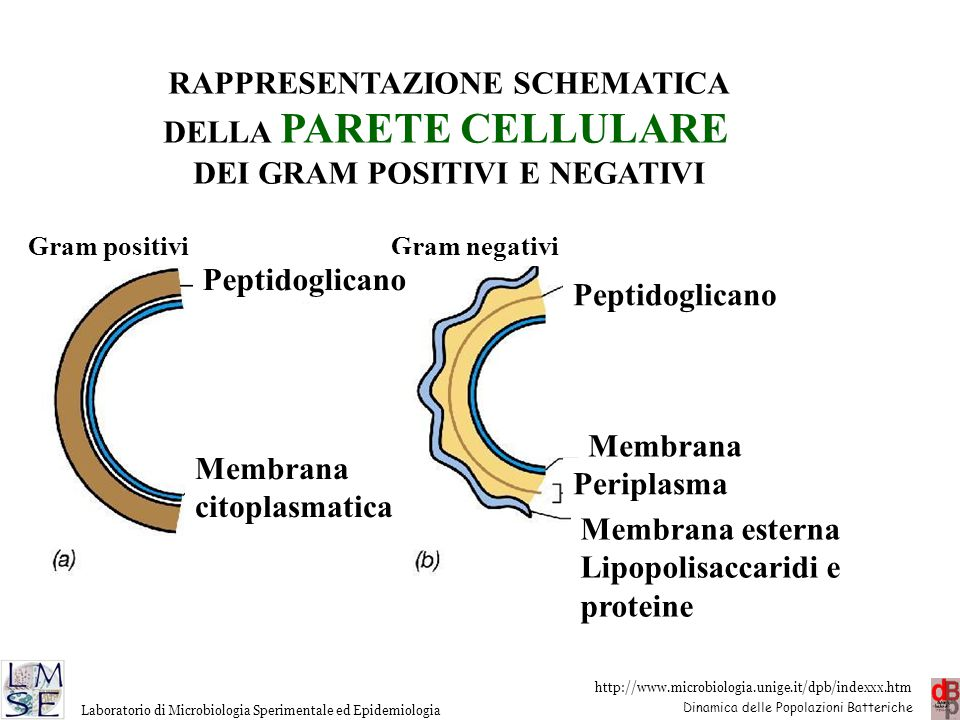
\includegraphics[scale=0.40]{img/Parete_cellulare.jpg}
\caption{Differenze nella membrana tra batteri Gram+ e Gram-}
\label{parete_cellulare}
\end{figure}


\subsection{Composizione della membrana plasmatica}
Nei batteri la membrana plasmatica è formata da una membrana fosfolipidica classica: un doppio strato fosfolipidico organizzato con le teste polari rivolte verso l'esterno e le code idrofobiche rivolte verso l'interno.\\

Esistono tuttavia delle differenze nella composizione tra la membrana dei Bacteria e quella degli Archea.\\

Nei \textbf{Bacteria}:
\begin{itemize}
\item La \emph{testa} del fosfolipide è formata da una molecola di \textbf{D-glicerolo-3-fosfato}. Al fosfato esterificato al C3 possono essere legati dei gruppi funzionali;
\item La \emph{coda} è costituita da \textbf{due molecole di acidi grassi esterificati} al C1 e C2 (in maggioranza sono \textbf{saturi}, con aggiustamenti dettati da variazioni ambientali);
\item Il gruppo fosfato è esterificato sul \textbf{C3}.
\end{itemize}

\vspace{1em}
Tipicamente, nelle membrane dei Bacteria sono assenti gli steroli (con l'eccezione dei metilotrofi), come il colesterolo, i quali sono sostituiti dagli \textbf{opanoidi}.
Gli opanoidi contribuiscono a stabilizzare la struttura e a renderla meno flessibile (svolgono la stessa funzione del colesterolo nelle cellule eucariote).\\

\clearpage
Negli \textbf{Archea}:
\begin{itemize}
\item La testa del fosfolipide è formata da una molecola di \textbf{L-glicerolo-3-fosfato}. I legami con le catene idrofobiche si formano al C2 e al C3;
\item Negli Archea il legame tra il glicerolo e le catene alifatiche, ovvero le catene di acidi grassi, sono \textbf{eteri} (e NON esteri)
\item Il gruppo fosfato è esterificato sul \textbf{C1};
\item Negli Archea le catene di acidi grassi sono costituite da catene di \textbf{isoprene} contenenti doppi legami.
\end{itemize}


\begin{figure}[htp]
\centering
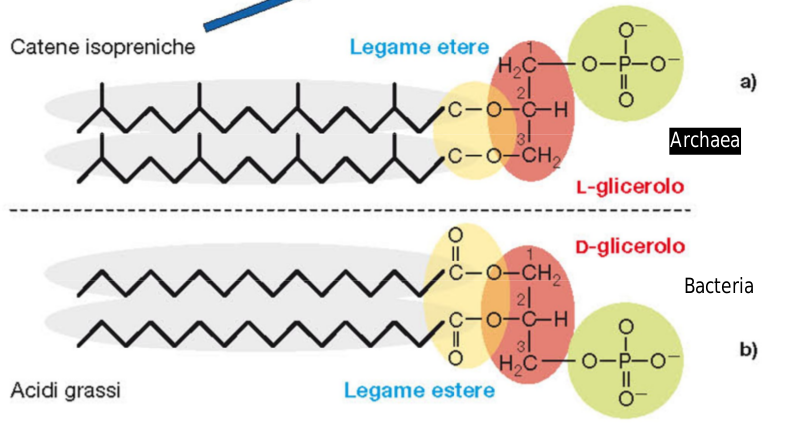
\includegraphics[scale=0.3]{img/Fosfolipidi.png}
\caption{Differenze nei fosfolipidi di Bacteria e Archea}
\label{}
\end{figure}

\vspace{1em}
I lipidi degli Archea possono essere \textbf{dieteri} (cioè con 2 catene alifatiche a 20C legate covalentemente al glicerolo) o \textbf{tetraeteri} (cioè 2 catene alifatiche a 40C legate a due molecole di glicerolo) del glicerolo. 

Negli Archea a volte non è presente un doppio strato fosfolipidico, ma un monostrato fosfolipidico il quale garantisce una maggiore stabilità alle membrane (si trova frequentemente negli Archea ipertermofili).

Questo monostrato si forma perché a volte la coda di \textbf{fitanile} di una molecola si collega alla coda di fitanile di un'altra molecola formando così un'unica molecola di \textbf{bifitanile} che fa sì che non ci sia più un doppio strato ma uno strato unico.

\begin{figure}[htp]
\centering
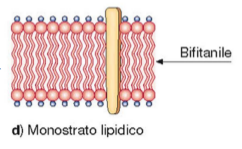
\includegraphics[scale=0.8]{img/Bifitanile.png}
\caption{Monostrato fosfolipidico}
\label{}
\end{figure}

\clearpage
Nelle membrane plasmatiche dei batteri, come in quelle eucaristiche, sono presenti anche delle proteine.
Queste possono svolgere ruoli di diverso tipo: possono formare canali, possono essere sensori di membrana, possono essere lipoproteine (nei Gram+ sono esposte verso l'esterno e nei Gram- sono esposte verso il periplasma), ecc...\\

Nella membrana di \emph{E. Coli} sono presenti oltre 200 tipi di proteine.

\subsection{Funzioni della membrana plasmatica}
\begin{itemize}
\item \textbf{Regolare la permeabilità}, rappresenta una barriera attraversabile solo da molecole piccole e non cariche e da molecole idrofobiche tramite diffusione;
\item \textbf{è il sito in cui sono collocate alcune proteine} che possono regolare il trasporto (formando canali), oppure possono modificare e trasferire un segnale alla cellula...;
\item \textbf{Produzione di energia}, respirazione e fotosintesi avvengono a livello di membrana. In entrambi i processi viene generato un gradiente ionico transmembrana (detta forza proton-motrice) che viene utilizzato dalla cellula per sintetizzare ATP;
\item \textbf{Biosintesi di componenti cellulari} come fosfolipidi, parti del peptidoglicano e del lipopolisaccaride.
\end{itemize}

\section{La parete batterica}

La parete batterica si differenzia per posizione e spessore tra Gram+ e Gram-: nei Gram+ è spessa, mentre nei Gram- è sottile e immersa nel periplasma.

Esternamente alla membrana citoplasmatica si trova una molecola polimerica chiamata \textbf{peptidoglicano} o \textbf{mureina}, la quale avvolge la cellula conferendole rigidità e forma.\\
Il peptidoglicano è formato da catene glicaniche costituite da due aminozuccheri alternati:
\begin{itemize}
\item il \textbf{NAG} (N-acetil glucosammina);
\item il \textbf{NAM} (Acido N-acetil muramico). Al NAM è legato un \emph{tetrapeptide} tramite il quale le catene glicaniche si connettono.
\end{itemize}

Tra questi due zuccheri vi è un legame $\beta$ 1-4 glucosidico che li lega in maniera successiva formando così delle lunghe catene.

\vspace{1em}
Legata al NAM, come già detto, c’è una catena di 4 amminoacidi. Per conferire ordine e resistenza alla struttura, il 3° amminoacido del NAM di una catena NAM-NAG si lega al 4° amminoacido del NAM di una catena parallela (questa viene detta struttura base).

\clearpage
\begin{figure}[htp]
\centering
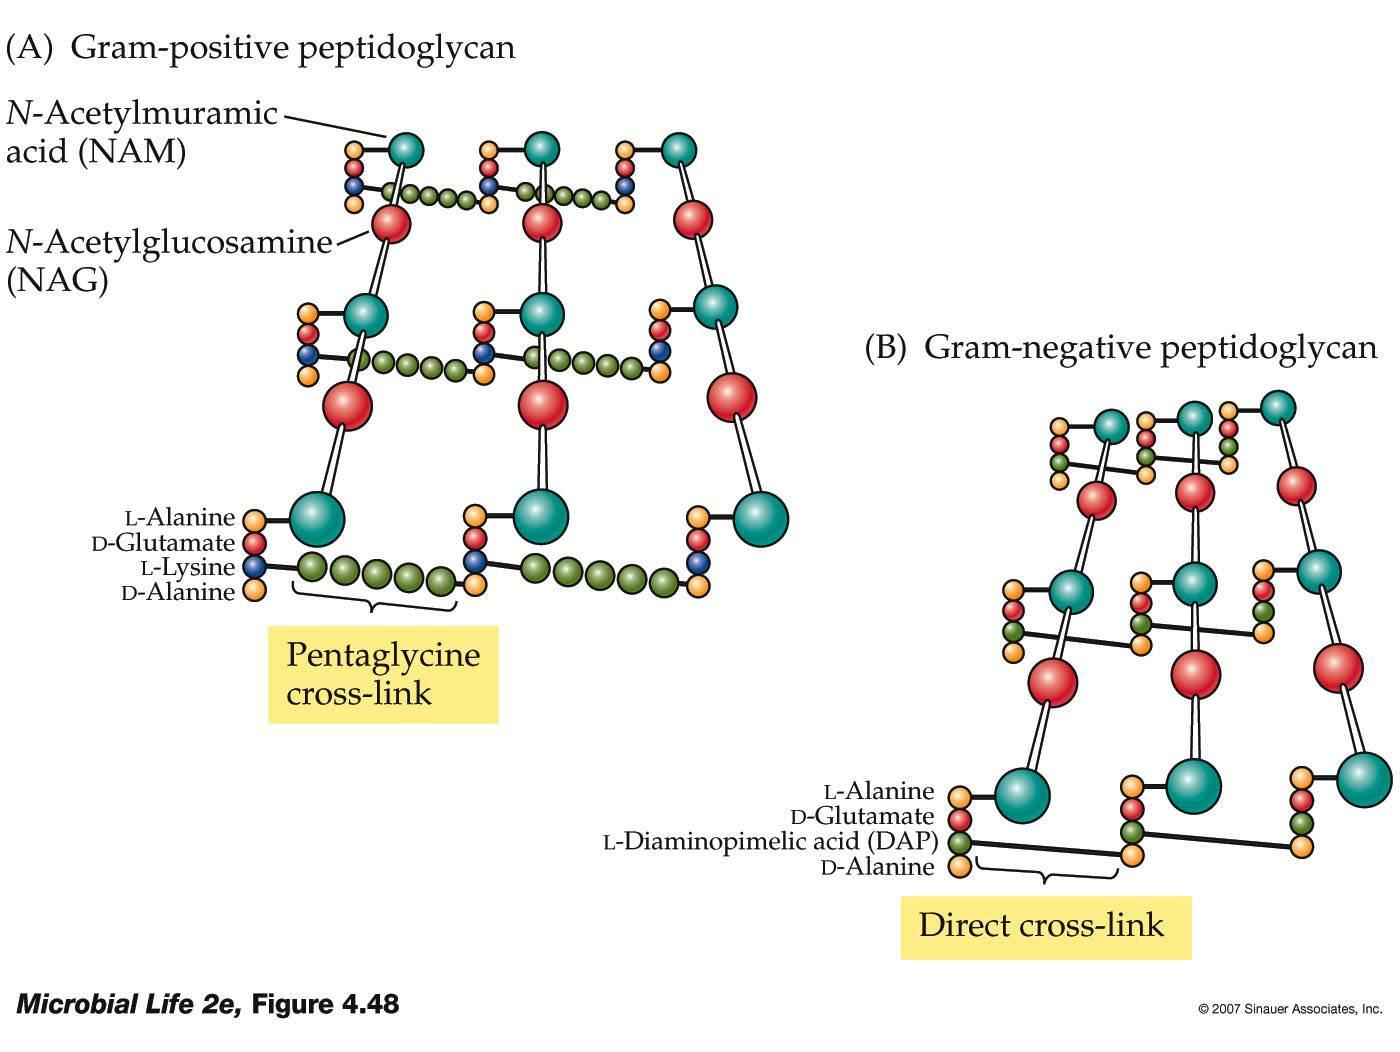
\includegraphics[scale=0.25]{img/NAM_NAG.jpg}
\caption{Legami nella parete cellulare}
\label{Legami parete cellulare}
\end{figure}

I Gram+ hanno una struttura più forte del peptidoglicano e resistono a temperature elevate più dei Gram-.

Questo avviene perché i Gram+ e i Gram- presentano delle differenze nel peptidoglicano: mentre nei Gram- il 3° e il 4° amminoacido sono legati direttamente tra loro, nei Gram+ il legame crociato non è diretto direttamente tra il 3° e il 4° amminoacido ma tra i due amminoacidi è inserita una \textbf{catena di pentaglicina}.\\
Un’altra differenza consiste nella sequenza dei 4 amminoacidi che per i G+ sono: 
\begin{enumerate}
\item L-Alanina;
\item D-Glutammato;
\item L-Lisina;
\item D-Alanina.
\end{enumerate}

Mentre nei G- i 4 amminoacidi sono:
\begin{enumerate}
\item L-Alanina;
\item D-Glutammato;
\item Acido L-Diaminopimelico (DAP);
\item D-Alanina.
\end{enumerate}

Questo significa che nei Gram+ il legame tra le catene avviene tra la lisina di una catena e l’alanina dell’altra, mentre nei Gram - il legame avviene tra l’acido L-Diaminopimelico e l’alanina.

\vspace{2em}
Il \textbf{lisozima} è un enzima presente nelle secrezioni biologiche come la saliva e le lacrime.
Questo enzima espleta un'azione antimicrobica grazie alla capacità di idrolizzare i peptidoglicani che formano la parete batterica. Il lisozima infatti è in grado di colpire i legami $\beta$ 1-4 tra gli zuccheri NAM e NAG.\\
In seguito alla lesione del peptidoglicano la cellula batterica inizia a richiamare acqua fino a scoppiare.


\subsection{La biosintesi del peptidoglicano}

la biosintesi del peptidoglicano avviene in tre differenti comparti della cellula:
\begin{enumerate}
\item nel \textbf{citoplasma}, dove vengono sintetizzati i \emph{precursori};
\item nella \textbf{membrana citoplasmatica}, dove avviene la sintesi dell’unità monomerica del glicano legato a un trasportatore lipidico e il suo ribaltamento sulla faccia esterna della membrana citoplasmatica;
\item nello \textbf{spazio esterno alla membrana} dove avvengono reazioni di polimerizzazione e transpeptidazione (si formano i legami crociati).
\end {enumerate}

La sintesi del NAG proviene da una trasformazione del \emph{Fruttosio-6-fosfato} con \emph{UTP} da cui si genera una molecola chiamata \textbf{UDP-NAG}.\\
A questo punto una molecola di \emph{PEP} viene trasferita al gruppo -OH dell’UDP-NAG da parte di \textbf{Mur A} formando un intermedio che viene poi trasformato da \textbf{Mur B} a \textbf{UDP-NAM}. \\
A questo punto intervengono altri enzimi chiamati \textbf{Mur C}, \textbf{Mur D}, \textbf{Mur E} e \textbf{Mur F}, i quali sono \emph{ligasi} responsabili dell’attacco della catena di amminoacidi al NAM (in questo momento gli amminoacidi sono 5, c’è un’Alanina supplementare).

\begin{figure}[htp]
\centering
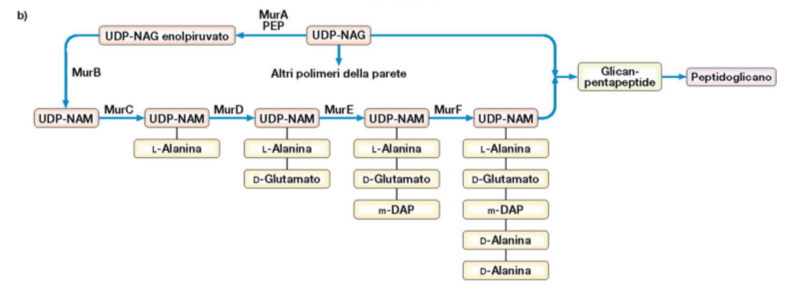
\includegraphics[scale=0.45]{img/Assemblaggio NAM.png}
\caption{Assemblaggio NAM}
\label{}
\end{figure}

A livello della faccia interna della membrana, si trova un trasportatore chiamato \textbf{bactoprenolo} (alcol a 55 C, idrofobo) che \emph{lega il NAM-pentammide} formando il \textbf{lipide I}. Successivamente al lipide I si lega un NAG e si forma il \textbf{lipide II}. A questo punto il bactoprenolo si ribalta sul lato esterno della membrana e diventa un substrato di \emph{transglicosilasi} che catalizza il legame tra il monomero nascente e il filamento nascente.\\
Successivamente si forma il legame peptidico tra la catena pentapeptidica del nuovo monomero e il tetrapeptide di una catena di glicano adiacente ad opera di \textbf{transpeptidasi}. \\
Infine il bactoprenolo viene defosforilato e ribaltato nuovamente sulla faccia interna della membrana.

\begin{figure}[htp]
\centering
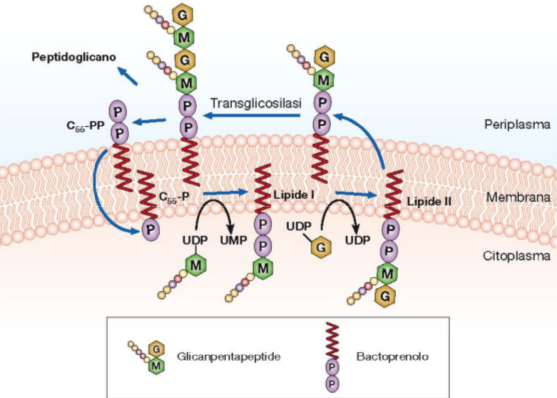
\includegraphics[scale=0.5]{img/Biosintesi peptidoglicano.png}
\caption{Biosintesi peptidoglicano}
\label{}
\end{figure}


\vspace{1em}
Tutta questa è una struttura molto complessa che ha dei punti deboli sui quali possono agire molti antibiotici. Ad esempio:
\begin{itemize}
\item la transpeptidazione può essere inibita da penicciline e cefalosporine;
\item la Bacitracina inibisce la defosforilazione del bactoprenolo;
\item cicloserina, inibisce la trasformazione di L-alanina in D-alanina...
\end{itemize}

Il peptidoglicano è presente unicamente nelle cellule batteriche. Per questo motivo gli antibiotici che vanno ad intaccare il peptidoglicano hanno una bassa tossicità: essi non possono intaccare le nostre cellule eucariotiche poiché esse non possiedono il peptidoglicano.

\subsection{La parete batterica dei Gram+}

Il rivestimento della cellula batterica dei Gram+, ovvero la parete batterica, costituisce il 40$\%$ del peso secco della cellula e ha uno spessore di 50 nm.\\
Contiene \textbf{acidi teicoici} e \textbf{lipoteicoici} i quali sono polimeri anionici.\\
Gli \emph{acidi teicoici} costituiscono il 60$\%$ della parete cellulare e si legano covalentemente allo scheletro polisacccaridico del peptodoglicano. Gli \emph{acidi lipoteicoici} invece, prendono contatto con la membrana citoplasmatica.
Queste molecole contribuiscono a fornire caratteri chimico fisici all’involucro, conferiscono carica superficiale negativa alla parete, e controllano il movimento degli ioni e dei cationi metallici.

\vspace{1em}
L'involucro esterno è costituito da una membrana a doppio strato e da uno spesso strato di peptidoglicano. Al peptidoglicano sono associati degli acidi che si differenziano per posizione, poichè quelli \emph{teicoici} sono immersi nel peptidoglicano mentre quelli \emph{lipoteicoici} fuoriescono dalla membrana. \\
Questi acidi hanno il compito di conferire alla cellula una carica negativa che consente al batterio di aderire alle argille grazie a interazioni elettrostatiche.\\
Mancano della membrana esterna.


\subsection{La parete batterica dei Gram-}
Il rivestimento della cellula battericadei Gram-, ovvero la parete batterica, consiste di un ottile strato di peptidoglicano circondato da una membrana esterna a doppio strato fosfolipidico. Questa membrana esterna tuttavia, ha una composizione diversa rispetto alle altre membrane biologiche.\\
Lo spazio compreso tra la membrana citoplasmatica e la membrana esterna viene chiamato \textbf{periplasma}

\vspace{1em}
Il preplasma è un comparto acquoso che può rappresentare il 20-40$\%$ del volume cellulare totale.

Al suo interno sono presenti proteine periplasmatiche coinvolte in: 
\begin{itemize}
\item acquisizione di nutrienti:
\item generazione di energia;
\item sintesi del peptidoglicano;
\item biogenesi della membrana esterna;
\item degradazione e inattivazione degli antibiotici.
\end{itemize}

La \textbf{membrane esterna} è particolare e viene detta asimmetrica poichè perchè presenta due strati con differente composizione: lo strato rivolto verso l'interno è formato da \textbf{fosfolipidi}, mentre lo strato esterno è formato da \textbf{lipopolisaccaridi (LPS) }in cui sono immerse le proteine di transmembrana.

I \emph{lipopolisaccaridi} sono molecole anfipatiche contenenti lipidi e residui saccaridici.

Questa molecola è costituita da:
\begin{itemize}
\item un \textbf{lipide A}, ovvero un \emph{dimero di NAG esterificato con due gruppi fosfato e 4-7 molecole di acido grasso};
\item un \textbf{Core}, ovvero una regione polisaccaridica suddivisa in 
\begin{itemize}
\item un \textbf{core interno}, una regione conservata contenente 1-3 molecole di \textbf{2-cheto-3-deossiottonato (Kdo)} e uno \emph{zucchero a 7C};
\item un \textbf{core esterno} dalla composizione variabile contenente zuccheri a 6-7C; 
\end{itemize}
\item un \textbf{Antigene O}, ovvero un \emph{polisaccaride} costituito da unità tetra o pentasaccaridiche che si estendono fuori dalla cellula.
\end{itemize}

Grazie ai gruppi fosfato e agli zuccheri carichi la superficie esterna è carica negativamente.

\vspace{1em}
L'antigene stimola la risposta immunitaria poiché quando entrano i microrganismi il sistema immunitario dell'organismo ospite reagisce con la produzione di anticorpi specifici.
Nei batteri patogeni l’LPS rappresenta dunque un fattore di virulenza in grado di evadere le barriere aspecifiche dell’ospite (fagocitosi e attivazione del complemento).\\
La \emph{catena laterale O} induce nell’ospite la produzione di anticorpi specifici, mentre il \emph{lipide A} attiva l’immunità innata con conseguente produzione di citochinine e risposta infiammatoria.

\clearpage
Nella membrana esterna inoltre sono presenti:
\begin{itemize}
\item \textbf{porine}, complessi costituiti da tre monomeri di proteine transmembrana con struttura a botte ($\beta$ barrel) la cui cavità centrale costituisce il canale, dotato di diametro variabile, attraverso il quale fluiscono molecole più o meno grandi;
\item \textbf{lipoproteine} che stabilizzano la membrana e sono coinvolte nel trasporto di nutrienti, nella resistenza agli antibiotici e nella trasduzione del segnale.
\end{itemize}

\subsection{La colorazione di Gram}
La colorazione di Gram si basa su 4 passaggi in cui si ha l’utilizzo di:
\begin{enumerate}
\item un colorante (cristal-violetto);
\item un fissante (LUGOL);
\item un preparato in proporzioni variabili di alcol e acetone;
\item un decolorante; 
\item un colorante di contrasto (safranina).
\end{enumerate}

\textbf{Procedimento}\\
Dopo aver formato una coltura di batteri:
\begin{enumerate}
\item toccare a colonia batterica con un bastoncino e stemperare la colonia rimasta sul bastoncino su un vetrino con una goccia d’acqua;
\item effettuare la fissazione al calore: passare il vetrino con i batteri e l’acqua su una fiamma per farne evaporare l’acqua. I batteri in questo modo muoiono e rimangono adesi al vetrino;
\item versare delle gocce di colorante cristal-violetto sul preparato. Questo colorante entra sia nei batteri G+ che in quelli G- conferendogli il colore viola;
\item fissare il colore tramite qualche goccia il LUGOL, dopodiché lavare le cellule per toglierne l’eccesso;
\item fissare il colore con il preparato di alcol-acetone. Questa soluzione entra solo nelle batteri Gram - decolorandoli, mentre non riesce ad entrare nei Gram+ a causa del peptidoglicano che, insieme al colorante, forma uno strato impermeabile;
\item aggiungere il colorante di contrasto, la safranina, che colora solo i batteri Gram -.
\end{enumerate}

\clearpage
\begin{figure}[htp]
\centering
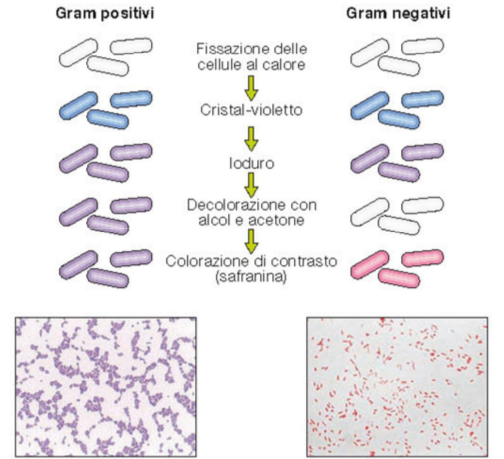
\includegraphics[scale=0.5]{img/Colorazione di Gram.png}
\caption{Colorazione di Gram}
\label{}
\end{figure}

Esistono poi dei batteri che vengono detti \textbf{Gram variabili}.\\
Alcuni batteri Gram+ (Arthrobacter, Actinomyces, Corynebacterium, Mycobacterium e Propionibacterium) infatti, rispondono in modo diverso alla colorazione di Gram in base alla loro fase di crescita: da giovani si colorano in maniera corretta, cioè esattamente come si colorerebbero i Gram+, mentre in una fase di crescita avanzata questi batteri assumono la colorazione dai Gram-. Questo avviene perché colture in fase di crescita più avanzata sono più fragili a livello del setto di divisione e rilasciano più facilmente il colorante.


\subsection{La parete batterica degli Archea}
Gli Archea non possiedono un vero peptidoglicano ma uno \textbf{pseudopeptidoglicano} (o pseudomureina) in cui il NAM è sostituito dal \textbf{NAT (Nacetil-talosaminuronico)} collegato a catene laterali di \emph{L-aminoacidi} (nel peptidoglicano sono presenti anche D-aminoacidi).\\
Gli amminozuccheri sono uniti da un legame $\beta$-1,3 anziché $\beta$-1,4.\\
Gli Archaea presentano una composizione di parete variabile a seconda del tipo di ambiente in cui vivono.

\section{Rivestimenti esterni delle cellule batteriche}
\subsection{Lo strato S o S layer}

Al di sopra dell’involucro esterno delle cellule batteriche, a volte, si può trovare lo strato S (o S layer).
Gli strati S sono costituiti da proteine insolubili in acqua che si assemblano a formare un reticolo cristallino di 5-25 nm. Le proteine che formano questo strato sono debolmente acide e legate a catene di glicani che sporgono all’esterno della cellula.\\
Di preciso non si sa che funzioni svolga questo strato ma certamente costituisce una barriere protettiva, promuove l’adesione cellulare, mantiene la rigidità cellulare, e nei batteri patogeni protegge dai meccanismi di difesa dell’ospite.\\
La capacità di un batterio di aderire al substrato può avere una notevole importanza clinica perché questi batteri possono aderire ai “medical devices” (come i cateteri) e causare infezioni nei pazienti.

\vspace{1em}
Lo stato S, a seconda della cellula batterica in cui si forma, può essere associato a diverse strutture della parete batterica:
\begin{itemize}
\item nei \emph{Gram+} e negli Archea è appoggiato al peptidoglicano;
\item nei \emph{Gram-} è appoggiato alla membrana esterna;
\item nei \emph{batteri privi} della parete cellulare lo strato S si appoggia direttamente alla membrana plasmatica (es. di batteri senza parete: i citoplasmi. Questi sono agenti patogeni che vivono nel floema delle piante, sono batteri vascolari e appartengono ad un gruppo tassonomico detto Mollicutes).
\end{itemize}
 
\subsection{Il glicocalice e la capsula}

Molti batteri rilasciano polisaccaridi che aderiscono alla superficie cellulare formando uno strato mucoso detto \textbf{glicocalice}. 
Se il glicocalice è ben strutturato e adeso alla parete cellulare viene definito \emph{capsula}, altrimenti, viene definito come \emph{slime layer}.\\ 
Batteri dotati di capsula hanno fenotipo mucoso, quelli privi di capsula hanno fenotipo rugoso.\\
Anche la capsula e il glicocalice svolgono un compito di protezione dell’organismo impedendogli d’entrare in contatto con le molecole antibiotiche, e proteggendoli dalla fagocitosi da parte di protozoi e di cellule del sistema immunitario.\\
Inoltre costituiscono un fattore di virulenza, e promuovono l’adesione ai substrati.

\vspace{1em}
La presenza della capsula può essere identificata tramite una colorazione negativa.

\chapter{Il movimento dei batteri}

I batteri si muovono nuotando, sciamando, strisciando, contraendosi o galleggiando grazie a strutture esterne o interne (flagelli, pili, proteine del citoscheletro, vescicole gassose o magnetosomi).\\
Queste strutture sono alla base di vari fenomeni di \textbf{tassia} che regolamentano il movimento dell'organismo verso siti favorevoli:
\begin{itemize}
\item \textbf{chemiotassi}, ovvero un movimento in risposta a stimoli chimici. Può essere: \emph{positiva}, se è presente una molecola gradita al batterio, o \emph{negativa} se il batterio si allontana in risposta ad una molecola dannosa;
\item \textbf{fototassi}, ovvero un movimento verso certe lunghezze d’onda della luce. È un movimento tipico dei batteri fotosintetici;
\item \textbf{aerotassi}, un movimento in risposta alla concentrazione dell’ossigeno;
\item \textbf{magnetotassi}, un movimento lungo linee di forza magnetiche;
\item \textbf{pHtassi}, un movimento in risposta al pH;
\item \textbf{termotassi}, un movimento verso una temperatura ottimale;
\item \textbf{osmotassi}, un movimento in risposta a concentrazioni ioniche.
\end{itemize}

\section{Strutture di locomozione batteriche: i flagelli.}

I flagelli, che costituiscono le appendici di locomozione principali, sono lunghe appendici cave formate da \textbf{flagellina} (una proteina) che grazie ad un movimento rotatorio permettono al batterio di muoversi.\\
I flagelli hanno un diametro di 10-20 nm, e una lunghezza di 5-20 µm.

\vspace{1em}
I flagelli possono essere:
\begin{itemize}
\item \textbf{monotrichi}, cioè singoli ad un polo della cellula; 
\item \textbf{anfitrichi}, cioè due disposti ognuno ad un polo della cellula; 
\item \textbf{lofotrichi}, cioè ciuffi di flagelli; 
\item \textbf{peritrichi}, cioè molti flagelli che circondano la cellula.
\end{itemize}

\clearpage
Il flagello è composto da tre parti:
\begin{enumerate}
\item un \textbf{corpo basale}, cioè una parte che ancora il flagello all’involucro cellulare e costituisce il motore cellulare. È formato da una serie di dischi (4 nei G- e 2 nei G+);
\item un \textbf{uncino}, cioè una breve struttura flessibile che connette il corpo basale al filamento;
\item un \textbf{filamento}, cioè una struttura semirigida tubulare con diametro di 20 nm e lunghezza di 10-15 µm, costituita da monomeri di flagellina.
\end{enumerate}

\subsection{Il flagello nei Gram-} 
Nei batteri Gram- il corpo basale è formato da 4 dischi i quali hanno nomi che rispecchiano il sito in cui sono situati, come visibile in fig. \ref{flagelli_gram-}.

Partendo dall’interno della cellula e dirigendoci verso l’esterno troviamo:
\begin{enumerate}
\item un \textbf{anello C}, localizzato nella parte interna della membrana plasmatica;
\item un \textbf{anello MS}, localizzato nella parte esterna della membrana plasmatica;
\item un \textbf{anello P}, associato al peptidoglicano;
\item un \textbf{anello L}, associato al LPS.
\end{enumerate}

Vi è dunque un anello per ogni settore della “copertura” della cellula.

\begin{figure}[htp]
\centering
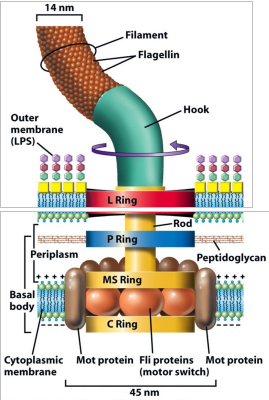
\includegraphics[scale=0.66]{img/Flagello.png}
\caption{Struttura dei flagelli nei Gram-}
\label{flagelli_gram-}
\end{figure}

Il \emph{``motore''} è costituito da subunità proteiche di \textbf{FliG}, \textbf{M }e \textbf{N}. Le proteine non rotanti che costituiscono lo \emph{``statore''} sono formate da proteine transmembrana (MotA e MotB).

Il flagello, a livello del corpo basale, è costituito da subunità proteiche chiamate MOT e FliG.
Le \textbf{MOT} circondano l’anello C e quello MS  formando lo statore, mentre le \textbf{FliG} ricevono un segnale (di magnetotassi, chemiotassi, ecc), ed impartiscono il movimento ai dischi.

Al di sopra degli anelli c’è l’uncino e poi il filamento.


\subsection{Il flagello dei Gram+}

Nei Gram+ i dischi sono solo due:
\begin{enumerate}
\item un \textbf{anello P}, associato al peptidoglicano;
\item un \textbf{anello M}, associato alla membrana plasmatica.
\end{enumerate}

\subsection{La sintesi del flagello}

La sintesi del flagello nei batteri è regolata da \emph{3 operoni} e \emph{60 geni}.
Essa si svolge in 3 fasi:
\begin{enumerate}
\item l’\textbf{operone di classe I (flhDC)} viene trascritto e si forma un complesso eteromultimerico che ha la funzione di sintetizzare una proteina con funzione di attivatore trascrizionale che attiva la trascrizione dell’operone di classe II;
\item l’\textbf{operone di classe II} attivato codifica per proteine strutturali del corpo basale e dell’uncino, e va ad attivare l’operone di classe III;
\item l’\textbf{opero di classe III} va a sintetizzare proteine del filamento (monomeri di flagellina), del motore flagellare MOT, e proteine per il sistema di trasduzione del segnale della chemiotassi.
\end{enumerate}

I monomeri di flagellina vengono sintetizzati nel citoplasma, passano all’interno del canale del flagello e si attaccano all’\emph{apice} dei monomeri del flagello in sintesi (autoassemblaggio).

\begin{figure}[htp]
\centering
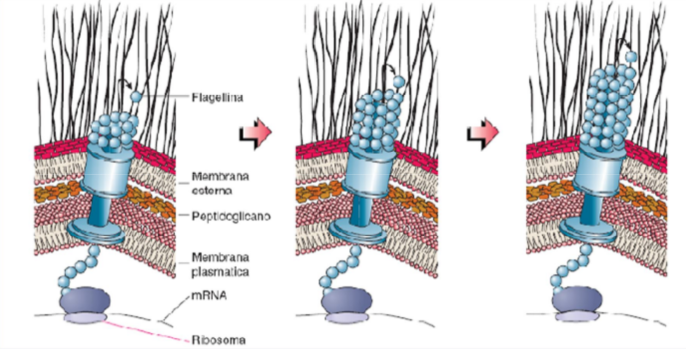
\includegraphics[scale=0.5]{img/Assemblaggio flagello.png}
\caption{Assemblaggio del flagello}
\label{}
\end{figure}

\clearpage
\subsection{Il movimento dei flagelli}

Il movimento di una cellula flagellata è impartito dalla rotazione del filamento:le cellule monotriche possono muoversi in avanti ruotando il flagello in senso antiorario, oppure indietro ruotando il flagello in senso orario. Nelle cellule peritriche o lofotriche (cellule dotate di più flagelli) invece, i flagelli devono essere un po’ riuniti e tutti coordinati nel fare la stessa cosa: se il batterio deve muoversi in avanti i flagelli si uniscono in fasci e danno forza propulsiva al batterio, mentre se il batterio deve cambiare la propria direzione i flagelli si aprono e ruotano in senso orario facendo sì che il batterio compia delle capriole che ne cambiano l’orientamento nello spazio.

\vspace{1em}
La produzione di energia, così come il movimento batterico, avviene grazie ad un flusso di protoni attraverso la membrana plasmatica che crea un gradiente di concentrazione \emph{(forza proton motrice)}: questo gradiente induce una \emph{modificazione strutturale nella proteina MotA} che circonda i dischi situati più all’interno della membrana.\\
Le proteine Mot imprimono un movimento rotatorio alle proteine FliG, le quali sono compattate fra i dischi MS e C. Questo movimento fa sì che lo spostamento dei dischi venga trasmesso all’albero motore, all’uncino, ed infine al flagello.\\
Il rotore può fare dai 6.000 ai 17.000 giri al minuto, ma il filamento arriva solo a 200 – 1.000 giri al minuto (rpm). Ogni giro richiede all’incirca lo spostamento di 1.000 protoni.


\subsection{I flagelli degli Archea}

Il flagello degli Archaea è simile a quello degli Eubatteri ma non del tutto uguale. 
Le principali differenze sono:
\begin{enumerate}
\item i flagelli batterici si muovono grazie ad una forza proton motrice, quelli degli Archaea si muovono grazie all’\emph{ATP};
\item le cellule batteriche hanno molti filamenti flagellari ognuno dei quali ruota indipendentemente, il flagello degli Archaea si compone di \emph{pacchetti di filamenti che ruotano come se fossero assemblati insieme};
\item I flagelli batterici crescono mediante aggiunta di monomeri di flagellina all’apice del flagello, quelli degli Archaea crescono per \emph{aggiunta di flagellina nella zona basale} e il flagello viene spinto fuori;
\item I flagelli batterici sono più spessi di quelli degli Archaea.
\end{enumerate}

\subsection{Batteri particolari: le spirochete (Gram-)}

Le spirochete sono batteri bastoncellari a forma elicoidale. 
Questi batteri possiedono un \textbf{flagello interno}, periplasmatico, invece che uno esterno.

Questa posizione del flagello rende il movimento delle spirochete particolare: esse “ruotano” su se stesse, attorcigliandosi come delle viti.

La rotazione dei filamenti flagellari induce la rotazione e la deformazione dinamica della cellula che spinge il batterio attraverso il fluido in cui si trova.
Nelle spirochete rigide (es. Treponema) la rotazione dei flagelli induce un movimento a spirale, mentre nelle spirochete flessibili (es. Borrelia) induce una curvatura e un movimento a spirale.

\begin{figure}[htp]
\centering
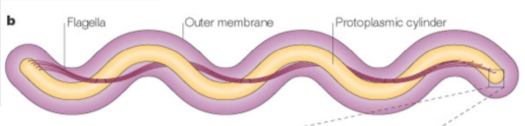
\includegraphics[scale=0.4]{img/Flagello Spirochete.png}
\caption{Il flagello periplasmatico delle Spirochete}
\label{}
\end{figure}

\section{La chemiotassi}
Con il termine ``chemiotassi'' si indica il processo migratorio di una cellula batterica innescato da un gradiente chimico di concentrazione.
La chemiotassi consiste nel movimento diretto verso una sostanza gradita, o lontano da una sostanza sgradita.\\
In presenza di un gradiente di sostanze repellenti o attraenti, la cellula misura a tempi diversi la concentrazione della sostanza nello spazio e trasduce il segnale al motore del flagello: se il batterio sente qualcosa di piacevole si sposta in direzione della sostanza, mentre se percepisce una sostanza sgradevole fa delle capriole per capire con precisione dove si trova la sostanza e poi fugge dalla parte opposta.
Se sono presenti entrambe le sostanze, una gradita e una nociva, la cellula risponde in base alla concentrazione delle due: se è maggiore quella buona si dirige verso di lei, se è maggiore quella negativa fugge.

Se si ha un \emph{aumento} della concentrazione della sostanza attraente, diminuisce la probabilità che la cellula compia una capriola allungando il percorso medio verso la concentrazione più favorevole.
Se si ha una \emph{riduzione} della concentrazione della sostanza attraente invece, aumenta la probabilità che la cellula compia una capriola e la lunghezza media del percorso nella direzione sfavorevole si accorcia.

\vspace{1em}
I sensori della sostanza chimica sono detti \textbf{chemorecettori} (proteine metil accettrici, MCP) e si spostano in direzione della sostanza gradita o sgradita.
Questi sensori sono \emph{proteine transmembrana} con il compito di percepire la presenza di alcune sostanze e trasmettere questa informazione al flagello, così che questo possa iniziare a ruotare.\\
In E. Coli sono state identificate 5 MCP. Ognuna di queste proteine transmembrana può rilevare una varietà di composti. Per esempio, il trasduttore Tar di E. Coli può percepire come attraenti sia l'aspartato che il maltosio e come repellenti metalli pesanti come il cobalto e il nichel.

\vspace{1em}
In presenza di una \emph{sostanza attrattante} il \textbf{recettore CheA}, una proteina transmembrana, viene inibito. A questo punto la presenza del \textbf{recettore CheY}, posizionato vicino al motore del flagello, aumenta, e il batterio si muove in \emph{senso antiorario} (ovvero in avanti).

\vspace{1em}
In presenza di una sostanze repellente invece, il recettore CheA va incontro ad un processo di \emph{autofosforilazione}. Successivamente avviene un \emph{trasferimento del gruppo fosfato} sul recettore CheY e CheB. A questo punto CheY-P interagisce con la \textbf{proteina FliM} promuovendo la rotazione del flagello in \emph{senso orario} (ovvero indietro).\\
Una volta che il batterio si trova lontano dalla sostanza repellente il \textbf{recettore CheZ} defosforila CheY bloccando la rotazione in senso orario.

\clearpage
\begin{figure}[htp]
\centering
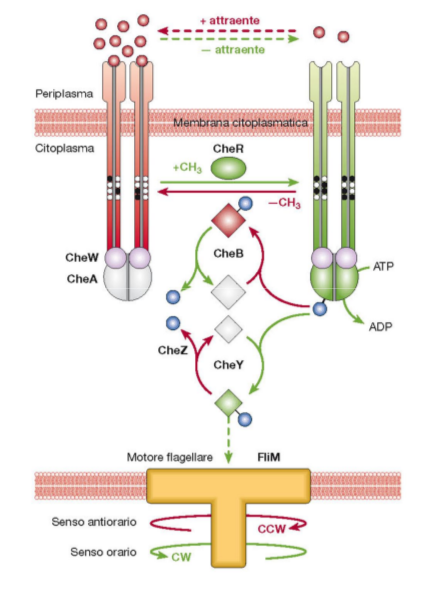
\includegraphics[scale=0.5]{img/Recettori chemiotassi.png}
\caption{I recettori della chemiotassi}
\label{}
\end{figure}

\subsection{Swimming e Swarming}

Le cellule batteriche possono cambiare sia la velocità sia la direzione della rotazione dei flagelli e quindi hanno varie forme di motilità.\\
Quando un batterio si sposta in avanti in una sola direzione per un certo periodo di tempo, il movimento viene detto ``running motility'', oppure \textbf{``swimming motility''}. Questo movimento è interrotto da bruschi cambiamenti casuali di direzione, detti ``capriole'', causate da un'inversione della rotazione dei flagelli, durante la quale il fascio dei flagelli si disgrega e la cellula inverte la sua direzione.

\clearpage
\begin{figure}[htp]
\centering
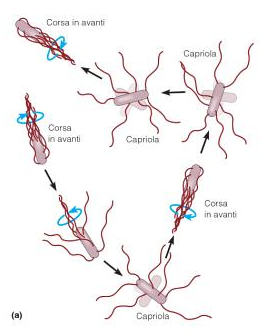
\includegraphics[scale=0.6]{img/Swimming e capriole.png}
\caption{Swimming e capriole}
\label{}
\end{figure}

Un altro tipo di motilità batterica  consiste invece nello \textbf{``swarming''}, ovvero in una traslocazione multicellulare.

Questa motilità, indotta dal contatto con superfici aventi un'appropriata viscosità e composizione, è caratterizzata dal \emph{differenziamento di cellule vegetative in cellule swarm}, lunghe ed iperflagellate.

La mobilità per scivolamento, detta anche \emph{gliding motility}, è il movimento dei procarioti \underline{non} dotati di flagello.
\`E una mobilità meno rapida che però permette al batterio di avere comunque una certa oppurtunità di movimento nel sito di locazione.


\section{Pili e fimbrie}
I pili, più lunghi, e le fimbrie, più corte, sono corte \textbf{appendici non flagellari} coinvolte in fenomeni di adesione a superfici cellulari e non, interazione tra cellule, secrezione, formazione di biofilm, coniugazione e movimento.\\
Alcune proteine, dette \textbf{adesine}, sono presenti all'estremo libero delle fimbrie e gli conferiscono potere adesivo alle fimbrie stesse, una specifica capacità di legarsi a peculiari substrati.\\
I pili invece, sono strutture con diametro di 5-9 nm e lunghezza di 1-4 $\mu$n che si estendono ai poli delle cellule.

I \emph{pili} sono strutture lunghe, ma più corti rispetto ai flagelli, mentre le \emph{fimbrie} sono più corte dei pili.

Entrambi non sono strutture flagellari e sono coinvolti sia nel contatto con superfici (soprattutto le fimbrie) sia nel contatto con altre cellule (soprattutto i pili).

\vspace{1em}
Alle fimbrie sono connesse proteine che mediano l'adesione ad ambienti particolari.\\


\subsection{La sintesi dei pili}
I pili sono strutture proteiche costituiti da monomeri di \textbf{pilina} organizzata in una struttura elicoidalei. I monomeri di pilina sono sintetizzati nel citoplasma, traslocati verso il periplasma, e qui assemblati attraverso la \textbf{proteina PilB}, una proteina con attività ATPasica, che causa una spinta del pilo verso l’esterno e la conseguente formazione di un vuoto che verrà subito riempito da una nuova subunità di pilina.

\begin{figure}[htp]
\centering
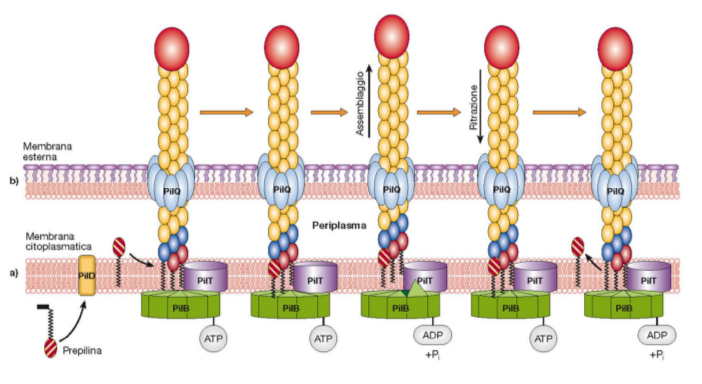
\includegraphics[scale=0.4]{img/Sintesi pili.png}
\caption{La sintesi dei pili}
\label{}
\end{figure}

In questo processo consorrono anche altre proteine come la \textbf{proteina PilQ} che forma un canale nella membrana esterna che permette il passaggio del pilo, la \textbf{proteina PilT} che un'attività antagonista rispetto a PilB e causa la rimozione di monomeri di pilina determinando la retrazione del pilo.\\
Estensione e retrazione del pilo mediati da PilT e PilB sono alla base del \emph{movimento contrattile (Twiching motility)} e della \emph{motilità per scivolamento (gliding motility)}.


\vspace{1em}
Molti procarioti sono mobili anche in assenza di flagelli, muovendosi attraverso una superficie solida mediante un processo di \emph{scivolamento}. La motilità per scivolamento è considerevolmente più lenta di quella a propulsione mediata dal flagello, ma permette comunque al microrganismo una certa possibilità di movimento nel suo habitat.\\
La morfologia delle colonie dei batteri che si muovono per scivolamento è del tutto caratteristica, con cellule che si spostano fuori dal centro della colonia stessa.

\chapter{Il protoplasto}

Con il termine \emph{``protoplasto''} si indica l'insieme di:
\begin{itemize}
\item citoplasma; 
\item membrana plasmatica;
\item nucleoide;
\item corpi di inclusione.
\end{itemize}

\section{Il citoplasma}
All'interno della cellula batterica si trova il \emph{citoplasma}. Questo è composto da acqua (ne rappresenta l'80$\$\%$), proteine, amminoacidi, acidi nucleici e substrati.\\
Il citoplasma ha una \emph{struttura granulare} data dalla presenza di un numero elevato di ribosomi (20.000-200.000 ribosomi in E. coli a seconda della fase di crescita). Il numero di ribosomi presenti varia a seconda della fase di crescita della cellula, quindi con il massimo della crescita si ha anche un massimo di concentrazione delle strutture ribosomiali \\
Nel citoplasma è contenuto del \emph{materiale genetico crosomiale} rappresentato dal \emph{DNA circolare} ed eventualmente dal \emph{DNA plasmidico}, che aggiunge delle caratteristiche di maggior adattamento all'ambiente. Il materiale genetico \emph{non è compartimentizzato}, quindi si trova sparso nel citoplasma ed è più addensato nel nucleoide.\\
Nel citoplasma si trovano \emph{organelli cellulari}, in particolare i ribosomi che sono dediti alla sintesi proteica. Nel loro complesso i ribosomi batterici sono \textbf{70S} (50S è la subunità maggiore e 30S è quella minore) e possono essere \emph{immersi nel citoplasma} (sintetizzano le proteine che non possono essere rilasciate all'esterno della cellua),oppure essere \emph{legati alla membrana plasmatica} (sintetizzano proteine che possono essere rilasciate all'esterno della cellula).\\
Infine nel citoplasma si possono trovare dei \emph{corpi inclusi} con la funzione di essere dei ``granai'' delle cellule batteriche, perchè immagazzinano sostanze che possono essere utilizzate in tempi di carestia.


\section{Il nucleoide}
Il nucleoide è quella zona della cellula contenente il materiale genetico (cromosoma + plasmidi) tipicamente non compartimentalizzato. 

\section{I ribosomi}
I ribosomi sono strutture ribonucleoproteiche (15-20 nm) coinvolte insieme a tRNA e mRNA nella sintesi proteica. I ribosomi possono essere citoplasmatici (deputati alla sintesi di proteine intracellulari), o legati alla membrana plasmatica (deputati alla sintesi di proteine destinate al trasporto all’esterno della cellula).

\section{I corpi inclusi}
I corpi di inclusione rappresentano dei depositi di sostanze di riserva. Le sostanze di riserva sono accumulate in presenza di nutrienti, e sono consumate quando in carenza di nutrienti.

\subsection{I granuli di riserva}
Tra i granuli di riserva troviamo:
\begin{itemize}
\item \textbf{granuli di glicogeno}. Questo è un polimero di glucosio con legami $\alpha$-1,4, e i granuli sono rivestiti da una membrana.
Il glicogeno conferisce alla cellula batterica una maggiore resistenza;
\item \textbf{granuli di polifosfato}. Questi granuli svolgono una funzione di riserva di fosfato per la sintesi di ATP e acidi nucleici;
\item \textbf{granuli di poli-$\beta$-idrossibutirrato (PHB)} e \textbf{poli-$\beta$-idrossialcanoato (PHA)}. Questi depositi di componenti di natura lipidica (unità ripetute di acido $\beta$-idrossibutirrico) sono stati riscontrati in Mycobacterium, Azotobacter e Bacillus. Questi organismi vengono utilizzati per produrre plastica biodegradabile;
\item \textbf{granuli di S}. Hanno una funzione di riserva di zolfo inorganico, derivato dall’ossidazione del solfuro. Sono una riserva energetica per la cellula batterica.
\end{itemize}

I CRISTALLI PARASPORALI svolgono un'attività insetticida e vengono utilizzati per la lotta biologica.

\subsection{Le vescicole gassose}

Le vescicole gassose sono strutture che consentono il galleggiamento della cellula micorbica. Il galleggiamento avviene tramito lo svuotamento della vescicola permettendo all'organismo di muovere un movimento verticale nel liquido. Il meccanismo di galleggiamento è connesso alla ricerca di condizioni ambientali ottimali.

\vspace{1em}
Le vescicole gassose sono costituite da due proteine \textbf{GvpA} (idrofoba forma nastri paralleli) e \textbf{GvpC} (aderisce a più nastri tenendoli uniti). All’interno racchiudono uno spazio cavo.\\

\begin{figure}[htp]
\centering
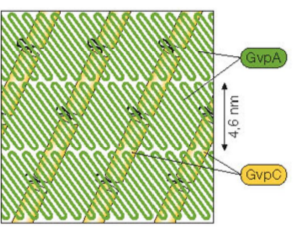
\includegraphics[scale=0.5]{img/Vescicole gassose.png}
\caption{Le vescicole gassose}
\label{}
\end{figure}

La proteina è costituita da circa il 50$\%$ di amminoacidi idrofobici disposti nella porzione interna dell’involucro che impediscono l’entrata dell’acqua ma facilitano quella dei gas.\\
Queste vescicole garantiscono il galleggiamento della cellula microbica permettendole di disporsi nei livelli d’acqua dove la luce, il tenore d’O$\ped{2}$ ed i nutrienti consentono il loro sviluppo.

\subsection{I magnetosomi}
I magnetosomi sono particelle cristalline intracellulari costituite da un ossido di Fe, la magnetite Fe$\ped{3}$O$\ped{4}$.I magnetosomi sono circondati da una membrana di fosfolipidi, proteine e glicoproteine. Si ritiene che le proteine di membrana svolgano un ruolo nella
precipitazione del Fe$\ap{3+}$ (trasportato nelle cellule in forma solubile da agenti chelanti) a Fe$\ped{3}$O$\ped{4}$.\\
I magnetosomi creano nella cellula un dipolo magnetico permanente, rendendola capace di rispondere ad un campo magnetico.\\

Il fenomeno della magnetotassi consiste dunque nella capacità del batterio di orientarsi e muoversi lungo le linee dei campi geomagnetici. 


\subsection{I microcomparti cellulari}
I microcomprati cellulari possono essere di diverso tipo. As esempio:
\begin{itemize}
\item \textbf{carbossisomi}, strutture che contengono l’\textbf{enzima ribulosio 1,5-difosfato carbossilasi (RuBiSco)} necessaria per fissare la CO$\ped{2}$ nei batteri autotrofi;
\item \textbf{granuli di cianoficina}, polipeptidi contenenti alte quantità di arginina ed acido aspartico. Sono una riserva di azoto;
\item \textbf{clorosomi}, presenti nei batteri verdi fotosintetici, i quali contengono le \textbf{batterioclorofille C, D, E} capaci di captare l’energia luminosa.
\end{itemize}

\clearpage
\chapter{Le endospore e il differenziamento cellulare}
Le \emph{endospore} sono strutture di resistenza della cellula batterica agli stress ambientali. le endospore sono resistenti ad agenti chimici come il cloroformio, il metanolo e l'etanolo, e fisici come T, pH, radiazioni...
Questi sono stress che normalmente rendono impossibile la vita per la cellula vegetativa. Le endospore non necessitano di acqua e nutrienti e persistono nel loro stato di quiescenza fino a che lo stress viene rimosso. I batteri che formano questo tipo di spore sono principalmente Gram+ come i Firmicutes a basso gc (Bacillus, Clostridium).

Esistono poi dei batteri che producono \emph{esospore}, cioè delle spore che vengono rilasciate all'esterno. Queste sono formate, ad esempio, dal micelio aereo degli Attinomiceti e permettono la colonizzazione di nuovi habitat.



\section{Il processo di sporulazione}
I batteri solitamente si dividono per \emph{scissione binaria} originando due cellule figlie uguali a quella madre.\\
Quando avviene la sporulazione invece, si attua un ciclo di divisione asimmetrica.
Quando si presenta una condizione di stress ambientale il batterio reagisce originando una zona, detta \textbf{setto di divisione} che indica la presenza del materiale genetico, e che divide la \textbf{prespora} dalla cellula madre. Prima della divisione asimmetrica il DNA si replica e sarà poi in grado di attraversare il setto di divisione.
All'interno della prespora il materiale gentico viene reso stabile e resistente a qualsiasi attacco fisico e chimico. La spora matura è poi pronta per essere rilasciata nell'ambiente ed è capace di resistere nel tempo.

\clearpage

\begin{figure}[htp]
\centering
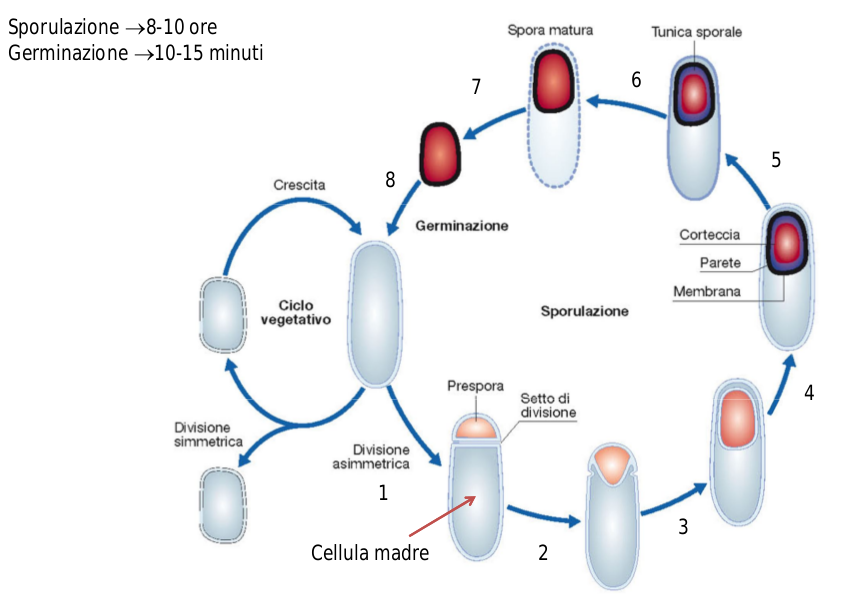
\includegraphics[scale=0.4]{img/Sporulazione.png}
\caption{Il processo di sporulazione}
\label{}
\end{figure}

L'induzione della sporulazione, in laboratorio, inizia alla fine della fase esponenziale (carenza di nutrienti e accumulo tossine).
Queste condizioni sono percepite dalla cellula mediante un sistema a più componenti detto \emph{multi component phosphorelay}, che determina l’attivazione di un \textbf{fattore trascrizionale (Spo0A)} e che induce la sporulazione.
Alcune cellule batteriche possono sporulare anche in condizioni di esaurimento delle risorse.

\vspace{1em}
Dopo la formazione della prepsora il processo di sporulaizone si svolge in più fasi:
\begin{enumerate}
\item \textbf{inglobamento della prespora} nella cellula. Il peptidoglicano nella zona del setto asimmetrico si degrada e il compartimento presporale si ingrossa, la membrana plasmatica della cellula madre si invagina migrando attorno alla prespora fino a inglobarla;
\item \textbf{formazione della corteccia}. Questo processo consiste nella sintesi di uno strato di corteccia formato da peptidoglicano con il 50$\%$  dei NAM privi della parte peptidica e ciclizzati nella forma lattamica. In seguito si ha la sintesi di \textbf{acido dipicolinico} che viene trasportato nella prespora accumulandosi come sale di calcio, stabilizzando gli acidi nucleici e conferendo termoresistenza alla spora. Infine si ha la sintesi di proteine acide a basso PM (SASP) che proteggono dai raggi UV;
\item \textbf{formazione del rivestimento esterno}. Intorno alla prespora si deposita la tunica sporale che conferisce resistenza a enzimi e agenti chimici;
\item \textbf{maturazione e rilascio della spora}. Questo processo avviene grazie alla lisi della cellula madre e al rilascio della spora. Le endospore mature hanno dimensioni di 0.5-1 $\mu$m. La parte cen trale (\emph{core)} della spora contiene il citoplasma disidratato che a sua volta è formato da RNA, DNA genomico, SASP e dipicolinato di Ca. In alcune specie l’endospora è rivestita anche da un esosporio.
\end{enumerate}

\clearpage
Infine si ha la \textbf{germinazione}: le spore metabolicamente inerti mantengono attivi i sistemi di ricezione del segnale che consentono di rispondere rapidamente ai segnali ambientali favorevoli diventando una cellula vegetativa.\\
Questo processo consta di diverse fasi: idratazione della spora, degradazione della corteccia, delle proteine SASP e della tunica sporale.

\begin{figure}[htp]
\centering
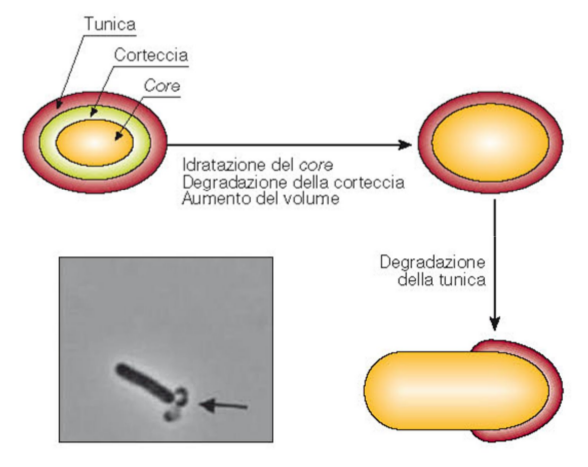
\includegraphics[scale=0.4]{img/Germinazione della spora.png}
\caption{Germinazione delle endospore}
\label{}
\end{figure}


\chapter{Nutrizione e crescita microbica}
\section{La crescita batterica}
La crescita microbica avviene tramite un meccanismo detto di \textbf{scissione binaria} che prevede la sequenza di diverse fasi.

\begin{figure}[htp]
\centering
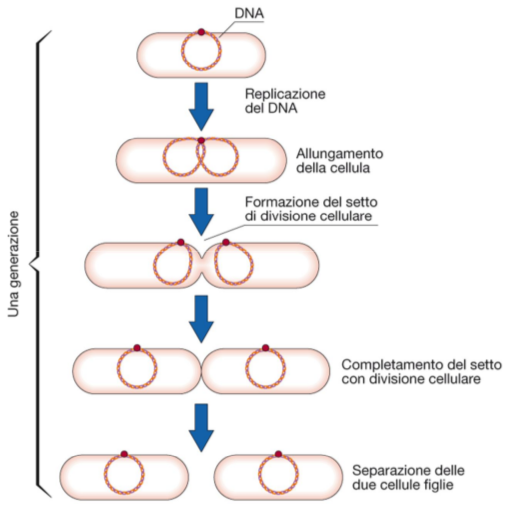
\includegraphics[scale=0.5]{img/Scissione binaria.png}
\caption{La scissione binaria}
\label{}
\end{figure}

\section{La composizione delle cellule batteriche}
Una delle condizioni necessarie affinchè avvenga la crescita batterica è la disponibilità di nutrienti.\\
I nutrienti necessari per la crescita microbica sono quelli di cui la cellula è costituita: 80- 90$\%$ acqua, H, C, O, N, P e S costituiscono il 95$\%$ del peso secco della cellula.

\subsection{I macronutrienti}
H, C, O, N, P, S, Fe, K, Ca, Mg e Na costituiscono il 99.5$\%$  del peso secco della cellula e per questo vengono detti \emph{``macronutrienti''}.\\
I macronutrienti sono i nutrienti necessari in alti quantitativi per la crescita microbica.

Tra questi troviamo:
\begin{itemize}
\item \textbf{carbonio (C)}. \`E il macronutriente più abbondante, costituisce lo scheletro di base delle molecole organiche.\\
In base alla fonte di C gli organismi si suddividono in:
\begin{enumerate}
\item \textbf{autotrofi}, usano \emph{C inorganico} (CO$\ped{2}$) come fonte di C. La (CO$\ped{2}$) subisce fissazione o organicazione del C mediante reazioni di riduzione;
\item \textbf{eterotrofi}, usano \emph{C organico }come fonte di C. La maggior parte dei microrganismi eterotrofi usa il C organico anche come fonte di energia (chemioorganotrofia).
\end{enumerate}

\item \textbf{ossigeno (O)} e \textbf{idrogeno (H)}, molto abbondanti nelle cellule. Per gli organismi eterotrofi la molecola organica funziona anche come fonte di H e O: gli autotrofi dalla (CO$\ped{2}$) ottengono O ma
non H che deve essere catturato da altre molecole. L’O$\ped{2}$ viene anche utilizzato nell’ambito della respirazione aerobica come accettore di elettroni durante la respirazione;
\item \textbf{azoto (N)}, rappresenta il 14$\%$ del peso secco cellulare. Si trova in proteine, acidi nucleici, fosfolipidi e polisaccaridi complessi (LPS, mureina). In natura si trova sotto forma di NH$\ped{3}$ (n.o. -3) e N$\ped{2}$ (n.o. 0), NO$\ped{2}$$\ap{-}$ (n.o. +3), NO$\ped{3}$$\ap{-}$ (n.o. +5). Il composto che viene acquisito direttamente e incorporato negli amminoacidi è l’NH$\ped{3}$. I microrganismi che usano altre fonti di N devono preventivamente effettuare la riduzione ad ammonio (riduzione assimilativa) per poterlo incorporare in molecole organiche;
\item \textbf{fosforo (P)}. Si trova in nucleotidi, acidi nucleici, fosfolipidi... In natura è sotto forma di fosfato che può essere assimilato direttamente;
\item \textbf{zolfo (S)}. Forma gruppi sulfidrilici SH- (n.o. -2) in cisteina e metionina. In natura si trova sotto forma di solfuro (H$\ped{2}$S $\ap{-}$, n.o. -2) , direttamente incorporato in molecole organiche, o come solfato (SO$\ped{4}$$\ap{-2}$, n.o. +6) che deve subire preventiva riduzione assimilativa a solfuro.
\end{itemize}


QUALSIASI MOLECOLA ORGANICA PRESENTE IN NATURA PUO’ ESSERE UTILIZZATA DA \underline{ALMENO} UNA SPECIE MICROBICA (INCLUSO MOLECOLE INQUINANTI).


\subsection{I micronutrienti}
Lo 0,5$\%$ restante è rappresentato da micronutrienti o elementi in tracce che sono richiesti in quantità infinitesimali e generalmente non vengono addizionati ai normali terreni di coltura.

\clearpage
\begin{figure}[htp]
\centering
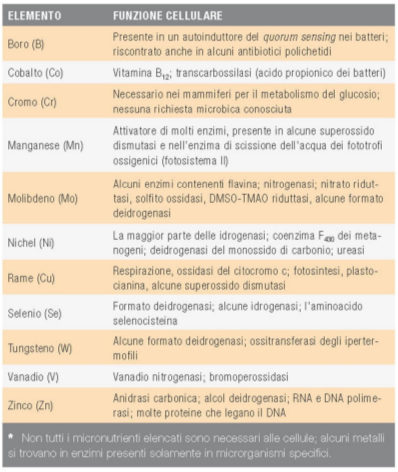
\includegraphics[scale=0.5]{img/Micronutrienti.png}
\caption{I micronutrienti}
\label{}
\end{figure}


\subsection{Analisi molecolare}
Macro e micronutrienti sono utilizzati dalla cellula per sintetizzare, mediante consumo di energia, macromolecole come proteine, polisaccaridi, lipidi, acidi nucleici (DNA e RNA).\\
Gli organismi viventi usano due forme di energia presente in ambiente: l’energia luminosa e l’energia derivante da reazioni di ossidazione di composti chimici organici ed inorganici.

\clearpage
\section{Le categorie nutrizionali}
le categorie nutrizionali possono essere due: carbonio ed energia.

\begin{figure}[htp]
\centering
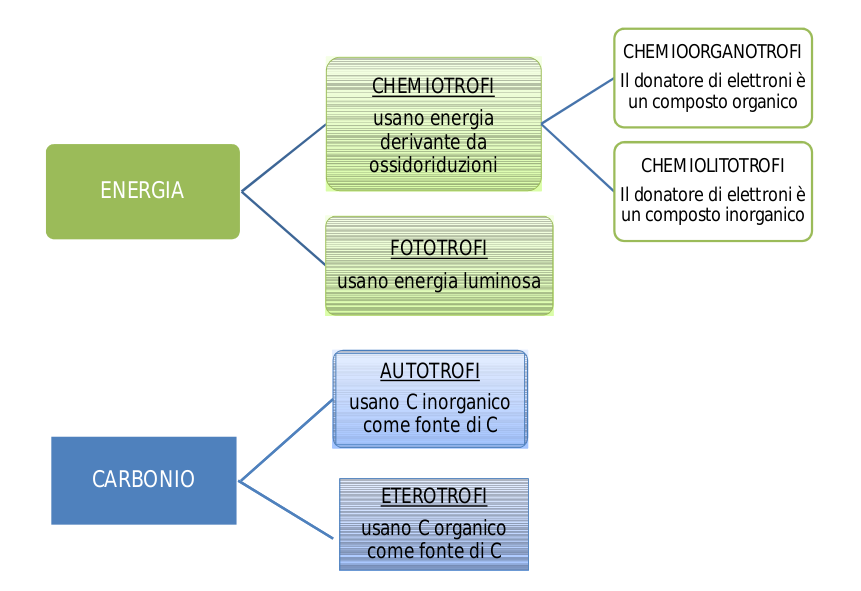
\includegraphics[scale=0.4]{img/Categorie nutrizionali.png}
\caption{Le categorie nutrizionali}
\label{}
\end{figure}

Combinando in modo diverso energia e C si ottengono diverse classi.

\begin{figure}[htp]
\centering
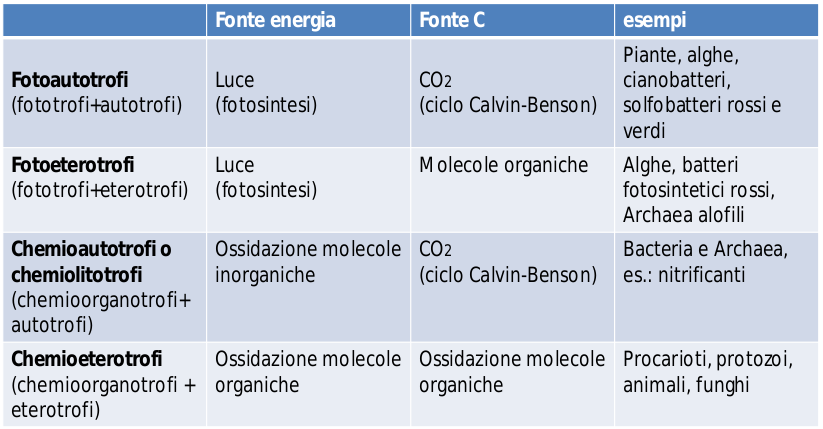
\includegraphics[scale=0.4]{img/Combinazioni energia e carbonio.png}
\caption{Classi}
\label{}
\end{figure}

\section{I fattori di crescita}
I fattori di crescita sono composti organici che la cellula richiede per crescere e che non è in grado di sintetizzare a partire dal C (es. aminoacidi, basi azotate, vitamine).\\
In laboratorio vengono utilizzati macro e micronutrienti ma alcuni batteri utilizzano fattori di crescita: questi batteri sono definiti come ‘fastidiosi’ perché difficili da far crescere in coltura.

I batteri si dividono dunque in due grandi categorie:
\begin{enumerate}
\item \textbf{protrotofi}, non necessitano di fattori di crescita e sintetizzano tutte le molecole organiche di cui necessitano a partire da un’unica fonte di C e minerali;
\item \textbf{auxotrofi}, richiedono fattori di crescita.
\end{enumerate}

\section{L'assimilazione dei nutrienti}
\subsection{La velocità di diffusione}
I nutrienti presenti nell’ambiente esterno devono essere internalizzati. Perchè questo avvenga i nutrienti devono oltrepassare la membrana esterna, il peptidoglicano (che in genere è piuttosto permeabile) e la membrana citoplasmatica. I due aspetti limitanti di questa operazione sono la velocità di diffusione attraverso lo strato fosfolipidico e la direzionalità del trasporto.

\subsection{La direzionalità del trasporto}
Il trasporto può avvenire \emph{secondo gradiente} (concentrazione del soluto maggiore nel comparto da cui parte il trasporto, non richiede energia) o \emph{contro gradiente} (concentrazione del soluto maggiore nel comparto verso cui arriva il trasporto, richiede energia).
Si muovono secondo un trasporto secondo gradiente H$\ped{2}$O, CO$\ped{2}$, N$\ped{2}$, O$\ped{2}$.

Il trasporto può anche avvenire mediante una \emph{diffusione facilitata} mediata da proteine integrali di membrana che formano pori che facilitano il movimento bidirezionale (es. acquaporine), o da permeasi che legano il soluto e lo spostano all’interno.

La velocità della diffusione semplice dipende dalla concentrazione del soluto (nel grafico linea retta).
Se il trasporto è mediato da proteine transmembrana avremo una fase iniziale in cui ci sono molto nutrienti all'interno e i trasportatori sono molti, dunque il trasporto sarà veloce (fase esponenziale). Successivamente però i trasportatori di membrana saranno saturati (tutti impegnati) e allora la velocità diminuirà. In un grafico questo risulterà come una curva in cui avremo una \emph{fase esponenziale iniziale} e quando i trasportatori saranno tutti impegnati avremo una \emph{fase costante} in cui ci saranno tanti nutrienti ma pochi trasportatori utilizzabili.

\begin{figure}[htp]
\centering
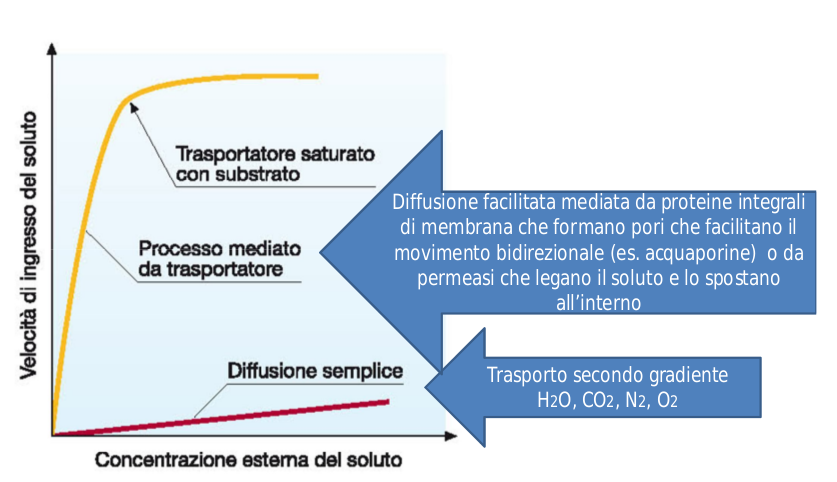
\includegraphics[scale=0.3]{img/Trasporto attraverso la membrana.png}
\caption{Trasporto attraverso la membrana}
\label{}
\end{figure}


\subsection{Le modalità di trasporto}
La diffusione facilitata può avvenire tramite specifiche proteine come le \textbf{porine}. Le porine sono strutture trimeriche che formano pori sulla membrana esterna: possono essere \emph{specifiche} (dedite al trasporto di un’unica tipologia di molecola) o \emph{aspecifiche} (trasportano differenti molecole aventi dimensioni adeguate).

\vspace{1em}
Il trasporto può essere:
\begin{itemize}
\item \textbf{attivo}, avviene cioé contro gradiente, richiede energia e proteine specifiche per il trasporto;
\item \textbf{passivo}, avviene secondo gradiente e perciò non richiede energia. Può essere semplice o avvenire sfruttando una proteina transmembrana. Si ha l'ingresso \underline{solo} del soluto.
\end{itemize}

\begin{figure}[htp]
\centering
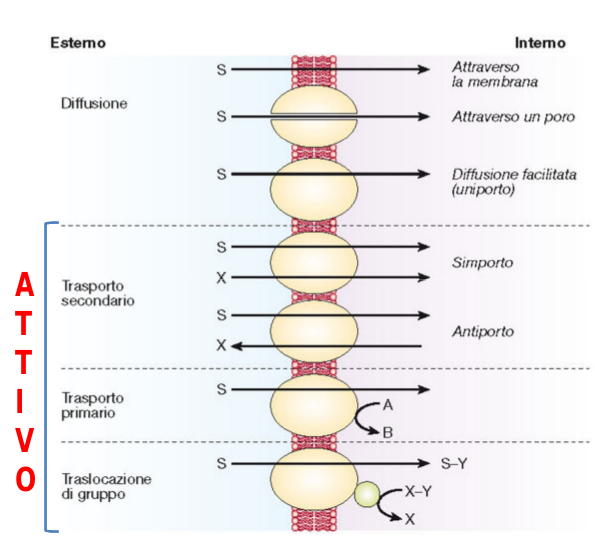
\includegraphics[scale=0.5]{img/Trasporto attivo e passivo.png}
\caption{Trasporto attivo e passivo}
\label{}
\end{figure}

Il trasporto tipicamente viene divisono in:
\begin{itemize}
\item \textbf{trasporto primario}. Il trasporto del soluto è accoppiato al consumo di energia derivante da metabolismo primario (idrolisi ATP, ossidoriduzioni, energia fotochimica).
Un tipico esempio sono i \textbf{trasportatori ABC}. Questi trasportatori sono costituiti da:
\begin{enumerate}
\item una proteina che idrolizza ATP associata alla membrana plasmatica; 
\item una proteina trasmembrana intergrale che funge da canale;
\item una proteina periplasmica con affinità per il substrato.
\end{enumerate}
Finora sono stati dentificati 200 trasportatori ABC specifici. 

\clearpage
\begin{figure}[htp]
\centering
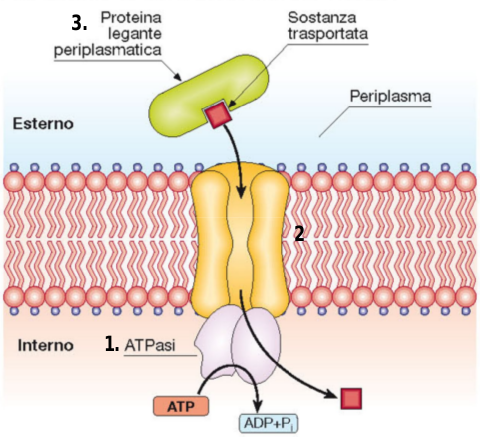
\includegraphics[scale=0.4]{img/Trasportatore ABC.png}
\caption{Trasportatori ABC}
\label{}
\end{figure}

\item \textbf{trasporto secondario}. La cellula usa l'energia potenziale di un gradiente elettrochimico (H$\ap{+}$, Na$\ap{+}$) generato da sistemi di
trasporto primario per trasportare molecole contro gradiente.\\
Il soluto può essere:
\begin{enumerate}
\item \textbf{co-trasportato (simporto)} con lo ione che fornisce l’energia per il trasporto;
\item \textbf{trasportato in direzione opposta (antiporto)} rispetto al movimento dello ione
\end{enumerate}

\item \textbf{traslocazione di gruppo}. Una molecola presente all'esterno della cellula viene trasportata all’interno di questa e contemporaneamente subisce una modificazione chimica.\\
Un esempio è il \textbf{sistema di fosfotransferasi (PTS)} in cui le proteine trasportatrici sono fosforillate e defosforillate determinando un trasporto a cascata del fosfato.\\
Per la traslocazione di gruppo del glucosio sono necessarie:

\begin{enumerate}
\item \emph{4 proteine citoplasmatiche:} EI, HPr, EIIa, EIIb
\item \emph{1 proteina integrale di membrana:} EIIc
\end{enumerate}

EI e HPr sono proteine aspecifiche, mentre EIIa, EIIb e EIIc sono specifiche per il glucosio.

Nel citoplasma della cellula la proteina \textbf{EI} riceve un PO$\ped{4}$$\ap{–2}$ dal PEP e lo cede alla proteina \textbf{HPr} la quale lo trasferisce a \textbf{EIIa}. Da EIIa il PO$\ped{4}$$\ap{–2}$ passa a \textbf{EIIb} e \textbf{EIIc}, che è il trasportatore di membrana. La proteina EIIc fosforilata riconosce il glucosio all’esterno e lo trasferisce all’interno cedendo il gruppo PO$\ped{4}$$\ap{–2}$. A questo punto dall'esterno della cellula arriverà una molecola di glucosio che potrà essere trasformata in glucosio-6-fosfato.\\
Per far sì che venga internalizzata una molecola di glucosio, il fosfoenolpiruvato (PEP)  deve cedere un gruppo fosfato alla proteina EI e trasformarsi in acido piruvico.

\clearpage
\begin{figure}[htp]
\centering
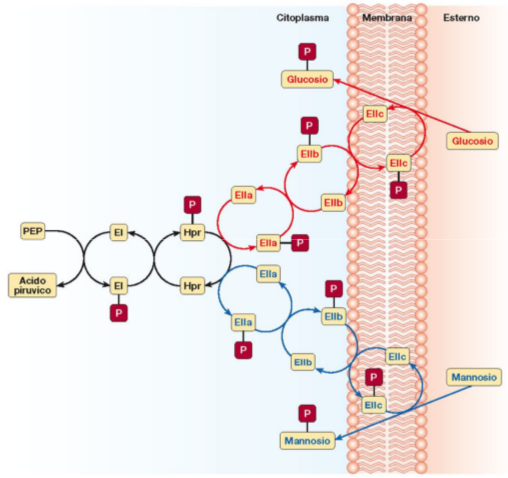
\includegraphics[scale=0.4]{img/Traslocazione di gruppo.png}
\caption{Traslocazione di gruppo del glucosio}
\label{}
\end{figure}

\end{itemize}


\section{La descrizione matematica della crescita batterica}
La crescita microbica avviene per scissione binaria con una progressione geometrica in base 2 in cui il numero di cellule raddoppia ad ogni generazione.\\
Il tempo necessario ad una popolazione cellulare per \emph{raddoppiare} il numero è detto \textbf{tempo di generazione}. Il tempo di generazione è costante per cellule dello stesso ceppo che si trovano nelle stesse condizioni di crescita.


\begin{figure}[htp]
\centering
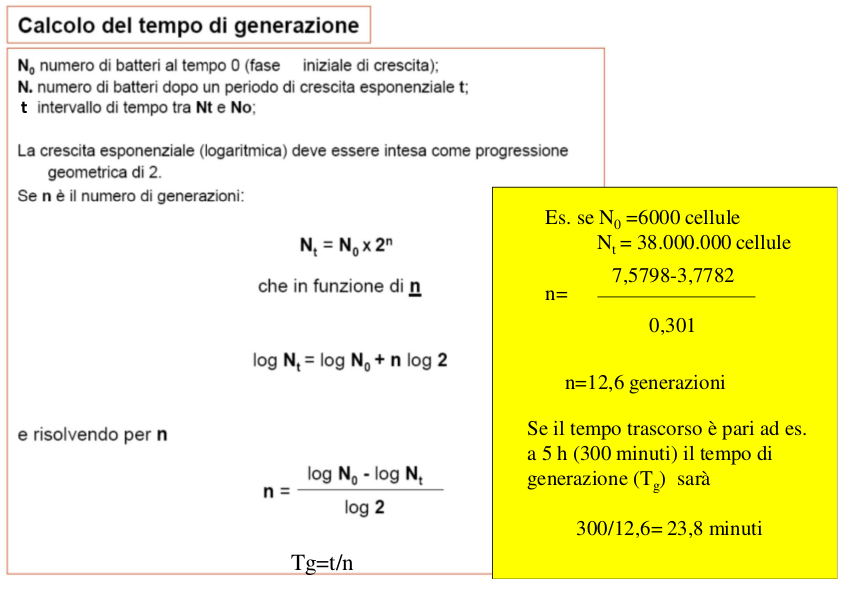
\includegraphics[scale=0.4]{img/Descrizione matematica crescita batterica.png}
\caption{Descrizione matematica della crescita batterica}
\label{}
\end{figure}


\subsection{La curva di crescita batterica in un sistema chiuso}
La crescita batterica in un sistema chiuso si ``divide'' in 4 fasi:
\begin{enumerate}
\item \textbf{Fase lag (latenza)}. In questa fase non si verifica un aumento numerico delle cellule, ma le cellule si adattano alle condizioni e al substrato di crescita sintetizzando gli enzimi necessari all’utilizzo dei
nutrienti. Questa fase può essere più o meno lunga in base al terreno di provenienza;
\item \textbf{Fase log (esponenziale)}. In questa fase il numero delle cellule aumenta alla massima velocità possibile. La velocità di crescita si mantiene costante e le cellule si dividono ad intervalli di tempo regolari. Durante questa fase si consumano i nutrienti e si accumulano sostanze di scarto e molecole segnale;
\item \textbf{Fase stazionaria}. In questa fase il numero di cellule non aumenta nel tempo perché le cellule smettono di dividersi, o perché viene raggiunto un equilibrio tra crescita e morte cellulare. Le cause che provocano questa stazionarietà sono: l'esaurimento di uno o più nutrienti, la carenza O$\ped{2}$ libero, l'accumulo di sostanze di rifiuto e l'elevata densità cellulare. Le cellule in fase stazionaria hanno dimensioni ridotte rispetto a quelle in fase esponenziale e maggiore capacità di resistenza agli stress (la carenza di nutrienti induce meccanismi di protezione cellulare che possono essere coinvolti anche nella resistenza ad altri stress);
\item \textbf{Fase di morte}. In questa fase si ha una riduzione numerica delle cellule che possono lisare o meno. Questa fase può essere più o meno rapida a causa dell'instaurarsi di meccanismi di resistenza in alcune popolazioni cellulari.
\end{enumerate}

\begin{figure}[htp]
\centering
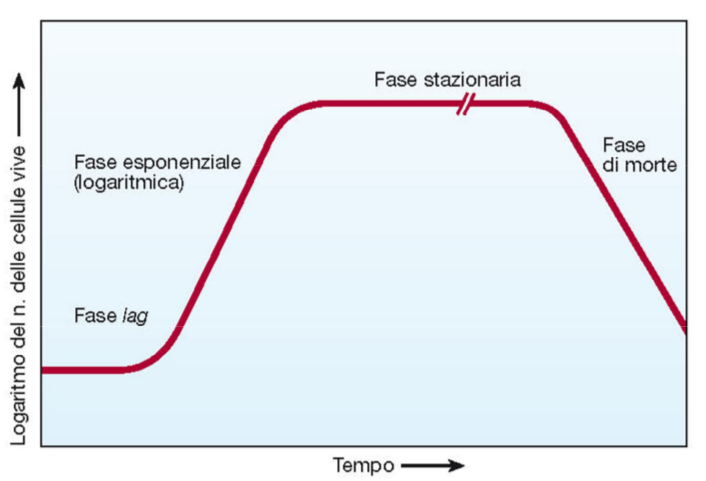
\includegraphics[scale=0.4]{img/Crescita batterica sistema chiuso.png}
\caption{Grafico di crescita batterica in un sistema chiuso}
\label{}
\end{figure}


In un sistema chiuso, in presenza di due fonti di C, si instaura una curva leggermente diversa da quella appena vista che viene detta \textbf{curva diauxica}. La caratteristica di questa curva è quella di presentare due fasi esponenziali successive intervallate da una fase di stasi.

\clearpage
\begin{figure}[htp]
\centering
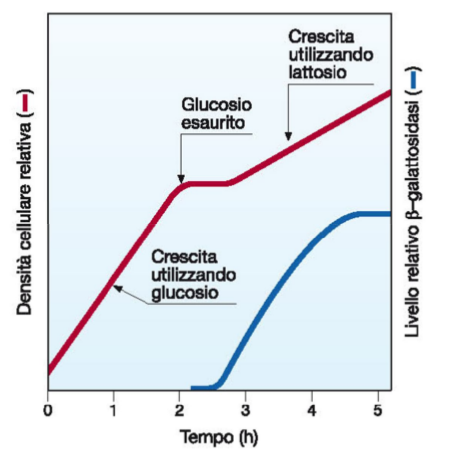
\includegraphics[scale=0.5]{img/Curva diauxica.png}
\caption{La curva diauxica}
\label{}
\end{figure}

\subsection{La crescita in continuo}
Lo sviluppo di colture in continuo consente di mantenere una coltura batterica in fase esponenziale per un periodo di tempo prolungato.
Per fare questo, ad una coltura in fase di crescita esponenziale, si addiziona una quantità di terreno fresco e se ne sottrae una equivalente di terreno usato (con cellule). In questo modo le cellule ricevono continuamente terreno fresco mentre i prodotti di scarto e le cellule sono continuamente rimosse.\\ 
Da questo processo si ottiene una crescita bilanciata in cui la biomassa, le concentrazioni di sostanze nutrienti e di metaboliti restano costanti detta \textbf{steady state}.

\clearpage
\subsection{Il chemostato}
\begin{figure}[htp]
\centering
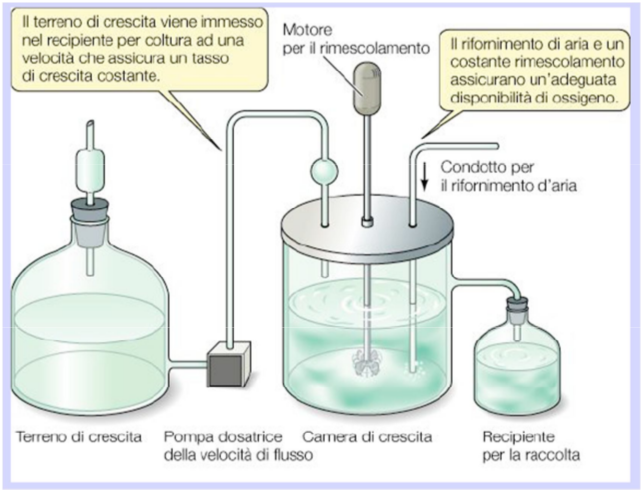
\includegraphics[scale=0.5]{img/Chemostato.png}
\caption{Il chemostato}
\label{}
\end{figure}

Il chemostato è uno strumento tramite il quale può essere effettuata la crescita in continuo. Il chemostato è formato da più parti e da più ``vaschette'' collegate tra loro.

Nel chemostato il terreno di crescita è collegato ad una pompa dosatrice della velocità del flusso, la quale a sua volta è collegata ad un recipiente, cioè la camera di crescita, che è collegata al recipiente di raccolta.

La camera di crescita è anche chiamata \textbf{bioreattore}. All’interno del recipiente di crescita si trovano dei batteri che crescono, e che una volta entrati nella fase esponenziale vi rimangono a lungo poiché viene continuamente addizionato del terreno di coltura nuovo che consente di avere nuovi nutrienti. Nella camera di crescita avviene poi un rimescolamento che mantiene adeguatamente ossigenati i batteri al suo interno.

Contemporaneamente, dalla camera di crescita, viene prelevata la stessa quantità di biomassa di terreno esausto (e di batteri) di quella immessa che finisce nel recipiente di raccolta.

Il controllo di un chemostato è delicato: la massima crescita cellulare coincide con la massima velocità di flusso dei nutrienti. Oltre a questo punto critico il tasso di diluizione supera il tasso di crescita e le cellule vanno incontro a dilavamento.

\clearpage
\begin{figure}[htp]
\centering
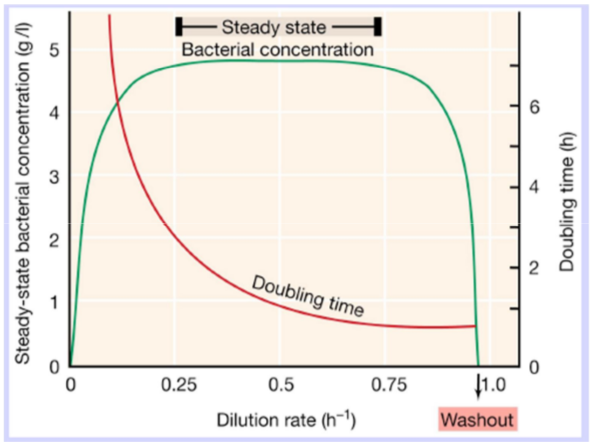
\includegraphics[scale=0.4]{img/DIlavamento.png}
\caption{Steady state}
\label{}
\end{figure}

La massima resa coincide con un T$\ped{g}$ (tempo di generazione) minimo.\\	
Il tasso di diluizione critico si presenta quando la velocità di diluizione è uguale al tasso di crescita.\\
Quando la linea rossa si incontra con quella verde si ottiene un punto chiamato \textbf{punto di washout}, questo è il punto in cui si ha la massima crescita cellulare, ma il tempo di generazione è minimo. 


\section{I terreni di coltura}
I terreni di coltura presentano al loro interno i nutrienti necessari per la crescita microbica.
Ne esistono di diversi tipi: 
\begin{itemize}
\item liquidi, detti anche brodi;
\item solidi, cioè agarizzati (l'agar è un polisaccaride).
\end{itemize}


Nei terreni liquidi si capisce se sono cresciuti dei batteri dalla torbidità del liquido, mentre nei per i terreni solidi si utilizzano le piastre di Petri per vedere i microrganismi sul terreno.

\subsection{I terreni di coltura solidi}
Questi terreno permettono di coltivare le cellule microbiche mantenendole separate spazialmente le une dalle altre.

Le cellule microbiche che si moltiplicano su un terreno solido danno origine a colonie visibili a occhio nudo che possono essere contate, caratterizzate e purificate.

I terreni di coltura solidi possono essere distinti in diversi gruppi:
\begin{itemize}
\item \textbf{terreni minimi}. Sono terreni di composizione nota che contengono il minimo dei nutrienti indispensabili per la crescita microbica: al loro interno si trovano sali e un'unica fonte di carbonio. La loro composizione è specie specifica, e la crescita su questi terreni è lenta. Vengono utilizzati per vedere la crescita di una sola specie microbica;
\item \textbf{terreni complessi}. Questi terreni contengono estratti di cellule vegetali o animali di composizione e in quantità non note. Sono usati per la crescita di molteplici gruppi microbici, e la crescita su questi terreni è rapida;
\item \textbf{terreni arricchiti}. Sono terreni complessi, liquidi o solidi, che possono essere addizionati con sangue, siero o altri complessi di nutrienti che favoriscono la crescita di \emph{determinati gruppi microbici}. Permette ottimi livelli di crescita a quei batteri che hanno esigenze particolari o sono numericamente non predominanti.\\ 
Un esempio di terreno arricchito è quello al selenio per l’isolamento delle salmonelle dalle feci (Brodo arricchimento selenite).

La formula tipica (g/l) di questo terreno è:
\begin{itemize}
\item triptone 5;
\item lattosio 4;
\item sodio fosfato bibasico 10;
\item sodio biselenito (NaHSeO$\ped{3}$)$\ped{4}$
\end{itemize}

Il sodio selenito possiede un'elevata tossicità, a pH neutro, per Escherichia Coli ma non per la maggior parte dei microrganismi appartenenti al gruppo delle salmonelle.

\item \textbf{terreni selettivi}. Sono terreni che consentono la crescita esclusiva di particolari gruppi microbici.\\
Esempi di terreni selettivi sono:
\begin{itemize}
\item \emph{Salmonella-Shigella Agar (SS-agar)}. Questo terreno contiene batteri fermentanti il lattosio che producono acido che, in presenza dell'indicatore rosso neutro, induce la formazione di colonie rosse. I batteri non fermentanti il lattosio invece, cioè la maggioranza dei patogeni intestinali (come Salmonella e Shigella), formano colonie incolori. Il tiosolfato di sodio e il citrato ferrico poi, consentono di evidenziare la produzione di solfuro di idrogeno da parte delle colonie grazie ad aree centrali di colore nero.\\
SU questo tipo di terreno la shigella genera colonie incolori, la Salmonella colonie incolori con il centro nero, mentre l'Escherichia Coli genera colorazioni rosa/rosso.
\item \emph{V.R.G.B. (Violet Red Bile Glucose Agar)}. Questo terreno è utilizzato per il conteggio e il rilevamento di enterobatteri nei cibi e in campioni biologici (contaminazione fecale). Il cristal violetto e i sali biliari presenti nel terreno inibiscono i batter Gram+. La degradazione del glucosio presente nel terreno induce il viraggio dell’indicatore di colore, il rosso neutro, e la formazione di un alone di precipitazione scuro intorno alla colonia. Gli enterobatteri formano colonie rotonde, color porpora e circondate da un alone scuro (diametro 1-2 mm);
\item \emph{agar cetrimmide}. Questo terreno viene utilizzato per l’isolamento e l’identificazione di Pseudomonas aeruginosa. Il digerito pancreatico di gelatina (o Peptone) contenuto nel terreno fornisce azoto, mentre il glicerolo è usato come fonte di carbonio ed energia.
La secrezione di piocianina è stimolata dal cloruro di magnesio e dal solfato di potassio contenuti nel terreno, mentre il cetrimide (cetiltrimetilammonio bromuro) è un composto dell'ammonio quaternario che inibisce la crescita di numerosi Gram+ e di alcuni Gram-, tra cui altre Pseudomonas spp. e microrganismi correlati. Questo terreno ha un basso contenuto di ferro.
\end{itemize} 


\item \textbf{terreni differenziali}. Questi terreni permettono di distinguere particolari gruppi microbici basandosi su caratteristiche metaboliche o morfologiche.\\
Esempi di terreno differenziale sono:
\begin{itemize}
\item il \emph{MacConkey agar}. Questo è un terreno differenziale e selettivo utilizzato per l’isolamento dei coliformi e dei patogeni intestinali nelle acque, nei prodotti alimentari e in campioni biologici.\\
I sali biliari e il cristal violetto presenti nel terreno inibiscono la maggior parte dei gram positivi (ad eccezione dei cocchi Gram+ quali stafilococchi ed enterococchi). La fermentazione del lattosio invece, causa
acidificazione del terreno con conseguente precipitazione dei sali biliari e del rosso neutro. I batteri coliformi e quelli fermentanti appaiono rossi con un alone scuro intorno, mentre i batteri non fermentanti sono incolori;
\item Terreni differenziali: questo terreno viene utilizzato per l'isolamento selettivo di stafilococchi e il rilevamento dello Staphylococcus aureus da campioni clinici. La presenza di NaCl al 7,5$\%$ inibisce parzialmente o del tutto gli organismi batterici diversi dagli stafilococchi.\\
La fermentazione del mannitolo, rivelata da un cambiamento dell'indicatore rosso fenolo, agevola la differenziazione delle specie di stafilococco: gli stafilococchi coagulasi-positivi (S. aureus) formano colonie gialle con terreno circostante dello stesso colore, mentre gli stafilococchi coagulasi-negativi (S. epidermidis)formano colonie rosse;
\item \emph{l'Agar sangue}. Questo terreno altamente nutritivo viene utilizzato per l'isolamento e la coltura di microrganismi esigenti e non esigenti estratti da campioni clinici. La presenza del sangue permette la determinazione dell’emolisi, criterio base per orientare l’identificazione batterica. Esistono 3 tipi diversi di emolisi:
\begin{enumerate}
\item BETA HEMOLYSIS (Streptococcus pyogenes). Si ha una emolisi totale, con formazione di una zona chiara attorno e sotto la colonia;
\item ALFA HEMOLYSIS (Streptococcus pneumoniae). Si ha una emolisi parziale, con la formazione di una colorazione verdastra attorno alla colonia;
\item GAMMA HEMOLYSIS, ovvero assenza di emolisi.
\end{enumerate}
\end{itemize}

(I terreni selettivi e differenziali sono utilizzati in campo chimico)
\end{itemize}

\section{La tecnica del trapianto di colture batteriche}
Il \emph{trapianto} viene usato per ottenere buone crescite batteriche, mentre l'\emph{isolamento} viene usato per ottenere colonie singole di cui verificare la forma e la purezza.

Sia per il trapianto che per l'isolamento si utilizzano delle anse con le quali si prelevano i microrganismi che vengono poi strisciati sulla piastra petri. Nell'isolamento però, ogni volta che si gira la piastra si flamba l'ansa per diluire la carica batterica ed arrivare ad avere colonie singole.

Un altro metodo è quello dello \emph{spatolamento} che ci permette di avere colonie distribuite uniformemente su tutta la superficie della piastra.

\clearpage
\section{Caratterizzazione delle colonie}
La caratterizzazione della morfologia delle colonie batteriche viene effettuata allo stereomicroscopio e si basa su 3 caratteristiche principali:
\begin{itemize}
\item Forma 
\item Spessore
\item Margine
\end{itemize}

\begin{figure}[htp]
\centering
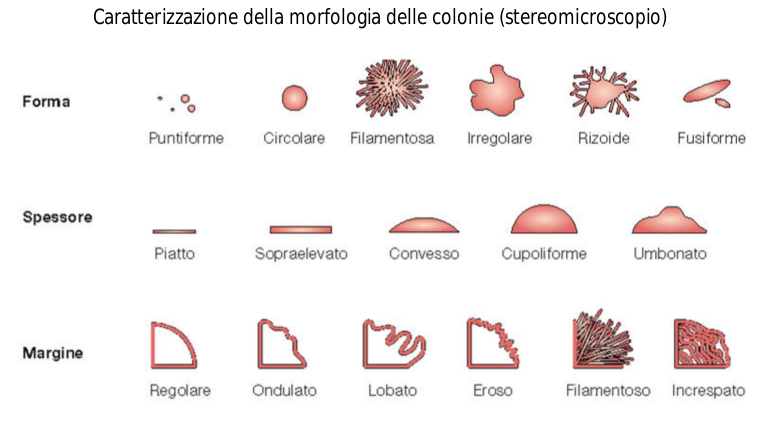
\includegraphics[scale=0.4]{img/Forma delle colonie.png}
\caption{Caratterizzazione delle colonie}
\label{}
\end{figure}

\section{Le tecniche di conteggio dei batteri in coltura}

Esistono due metodi di conteggio possibili:
\begin{itemize} 
\item \textbf{indiretti} (Coltura-Dipendenti).  \emph{vive} (non si ha il numero totale delle cellule). Esistono diversi tipi di conteggio indiretto:
\begin{enumerate}
\item \textbf{CONTEGGIO SU PIASTRA}. Questo metodo permette di conteggiare solo le cellule vitali e coltivabili. Si basa sull’assunto che ogni microrganismo vitale dia origine ad 1 colonia su un terreno di coltura.
Questo tipo di conteggio non sarà privo di errori in quanto i microrganismi possono aggregarsi, ed in quanto è fortemente soggetto ad errori dovuti all’operatore.\\ 
In questo metodo di conteggio non vengono considerati i microrganismi vitali ma non coltivabili (VBNC) e quelli con particolari esigenze nutrizionali.
L'espressione corretta per indicare questo metodo è \textbf{``conteggio CFU/ml''} (non cellule/ml). Il termine \textbf{``CFU''} (o UFC) sta per \textbf{unità formanti la colonia}.\\
Questo metodo di conteggio è fortemente legato alle \emph{``diluizioni seriali''}. Queste sono diluizioni 1:10 (1 ml in 9 ml di tampone = 500 $\mu$l in 4,5 ml di tampone, \emph{quindi 1 ml del composto madre diluito in 9 ml di tampone}. MAI DIRE  1: 10 = 1 ml in 10 ml!).
Queste diluizioni vengono fatte per separare le cellule in modo da essere contate facilmente.

\clearpage
\begin{figure}[htp]
\centering
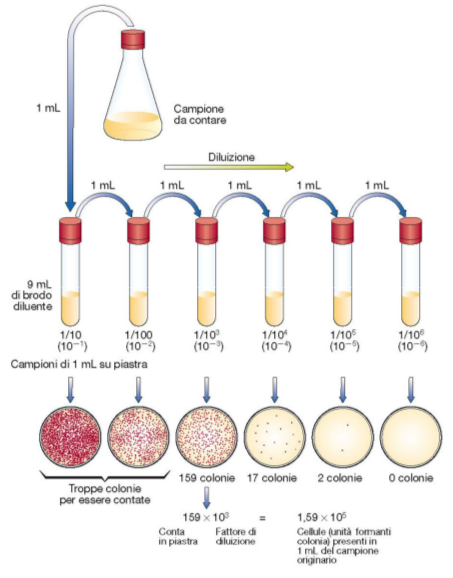
\includegraphics[scale=0.3]{img/Diluizioni seriali.png}
\caption{Diluizioni seriali}
\label{}
\end{figure}

Processo di diluizione seriale: si pone 1 ml del composto madre in 9 ml di brodo diluente ottenendo un composto 1/10. Dopodichè si preleva 1 ml del composto 1/10, e lo si immette in un’altra provetta con 9 ml di brodo ottenendo 1/100 e così via...
Per ogni diluizione faccio una piastra ed infine prendo in considerazione solo le piastre che hanno dai 20 ai 200 batteri.

\`E possibile calcolare il valore delle cfu/ml

\begin{figure}[htp]
\centering
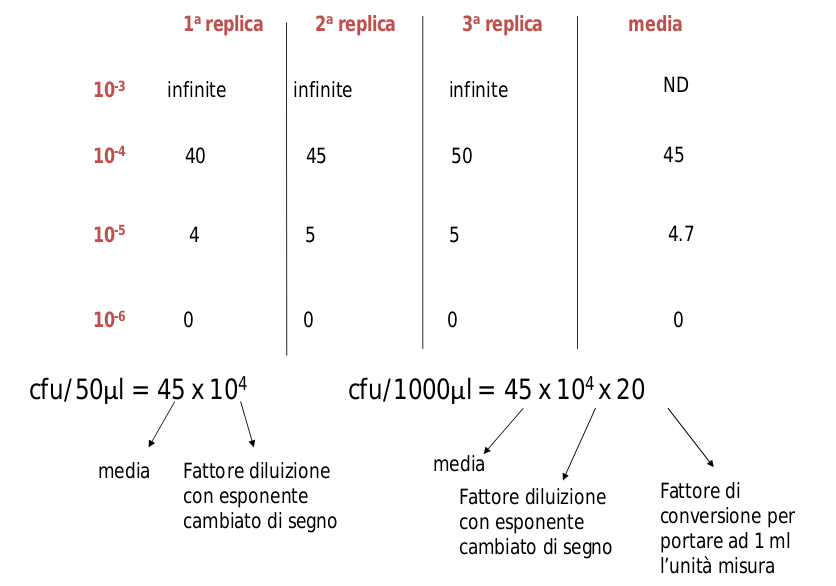
\includegraphics[scale=0.3]{img/Calcolo cfu-ml.png}
\caption{Calcolo delle CFU/ml}
\label{}
\end{figure}

\item \textbf{MPN (Most Probable Number)}. Questo metodo di conteggio permette di stimare il numero più probabile di microrganismi vitali capaci di proliferare nel mezzo di coltura.

Si inocula un campione d’acqua in quantità variabili in provette contenenti terreni selettivi diversi in relazione al microrganismo che si intende valutare e per ogni dose di campione si preparano più provette (3-5).
Per la supposta distribuzione casuale dei microrganismi nel campione, in una serie di tubi insemenzati con la stessa dose si potranno avere risultati diversi, e per questo si otterrà un livello di precisione tanto maggiore, quanto maggiore sarà il numero di tubi positivi.

\textbf{Principio del metodo:} realizzando diluizioni successive di uno stesso campione, esisterà almeno una diluizione in cui solo alcune aliquote della diluizione contengono microrganismi. Di conseguenza, inoculando più tubi, solo alcuni daranno luogo a crescita, mentre per le diluizioni precedenti tutti i tubi di inoculati con un’aliquota della diluizione daranno luogo a crescita, e per le successive tutti i tubi saranno sterili. Utilizzando il numero di tubi positivi in tre diluizioni successive è possibile risalire, mediante tabelle statistiche, al numero più probabile di microrganismi per ml o g di campione.

\textbf{Procedimento MPN:}
\begin{enumerate}
\item marcare le provette con il nome e la diluizione;
\item preparare le diluizioni del campione di acqua fino a 10$\ap{-7}$
\item seminare 1 ml di ogni diluizione in 3 provette contenti 9 ml di brodo lattosato doppio concentrato;
\item incubare a 37°C per 24 h;
\item si verifica la positività: la provetta viene considerata positiva quando c’è torbidità;
\item in base alla positività delle provette si ricava un numero a tre cifre detto \emph{numero caratteristico}.
\end{enumerate}

\textbf{Individuazione del numero più probabile di microrganismi:}
\begin{enumerate}
\item individuare la diluizione limite: è l’ultima diluizione, se esiste, con tutti i tubi positivi;

\begin{figure}[htp]
\centering
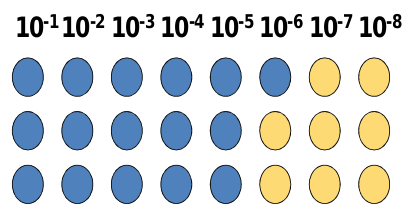
\includegraphics[scale=0.4]{img/Diluizioni MPN.png}
\caption{Diluizioni MPN}
\label{}
\end{figure}

\item individuare il \textbf{numero caratteristico:} è un numero a 3 cifre costituito dal numero di tubi positivi nella diluizione limite, dal numero di tubi positivi in quella successiva e poi ancora nella successiva: nell’esempio è 310;
\item ricavare dalle tabelle MPN il numero più probabile corrispondente al numero caratteristico: nell’esempio 4

\begin{figure}[htp]
\centering
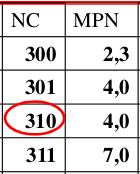
\includegraphics[scale=0.5]{img/Tabella MPN.png}
\caption{Tabella di determinazione del valore di MPN}
\label{}
\end{figure}

\item moltiplicare per il fattore di diluizione corrispondente alla diluizione limite: 4x10$\ap{5}$.
\end{enumerate}

\clearpage
I vantaggi di questo metodo sono:
\begin{itemize}
\item  è un metodo sensibile, perciò basta usare anche 50 ml di inoculo;
\item è facile da usare con substrati selettivi;
\item con particolari accorgimenti (come substrati fluorogenici) è possibile ottenere risultati in 4 h.
\end{itemize}

Gli svantaggi invece sono che:
\begin{itemize}
\item è molto meno preciso delle conte in piastra;
\item  è laborioso e può essere costoso.
\end{itemize}

\item \textbf{USO DELLE MEMBRANE FILTRANTI.}
\end{enumerate}


\item \textbf{diretti} (Coltura-Indipendenti). Con questo metodo si contano le cellule \emph{vive e morte} (si conta il numero di cellule vive e il numero di cellule morte quindi il numero totale delle cellule). Esistono diversi tipi di conteggio diretto:
\begin{enumerate} 
\item \textbf{CONTEGGIO AL MICROSCOPIO}, un volume noto di campione viene valutato in una camera di conta;
\item \textbf{CONTEGGIO SU VETRINO}, un volume noto di campione viene posto in un cm$\ap{2}$ di vetrino colorato. Si valuta il numero medio di m.o. presenti per campo ottico;
\item \textbf{USO DI COUNTER PER CELLULE} (es citofluorimetro);
\item \textbf{MISURAZIONE DELLA TORBIDITA’}, le cellule disperse in una coltura liquida possono bloccare (assorbanza) o diffondere (trasmittanza) la luce in proporzione alla loro massa. Le colture batteriche in brodo appaiono torbide perché le cellule diffondono la luce, entro certi limiti, in modo proporzionale alla loro densità.\\
La misura della torbidità si effettua attraverso uno spettrofotometro impostato con una lunghezza d’onda compresa tra 540 e 660 nm.
Una lampada emette luce con intensità I$\ped{0}$: a causa della diffusione, della rifrazione e dell’assorbimento arriva alla fotocellula per la luce trasmessa, un’intensità I.\\
I/I$\ped{0}$ è la \emph{trasmittanza} (0-100$\%$), mentre l’\emph{assorbanza} è log (I/I$\ped{0}$) e varia in genere fra 0 e 3. Per un intervallo limitato (0-0,6) esiste una relazione lineare fra l'assorbanza e il numero di cellule o biomassa del campione.
Il vantaggio di questo metodo di conta è che, anche se si ha una rapida riduzione cellule vitali in fase di morte, questa non è accoppiata ad una altrettanto rapida riduzione della torbidità (la biomassa non varia).
\item \textbf{VALUTAZIONI CHIMICHE}, si misura la massa cellulare valutando la quantità di N$\ped{2}$, proteine, P e ATP;
\item \textbf{VALUTAZIONE DEL PESO SECCO}, tramite processi di centrifugazione ed essiccamento (60 °C);
\item \textbf{VALUTAZIONE DEL VOLUME DELLA MASSA}, tramite centrifugazione
\end{enumerate}

\end{itemize}

\clearpage
** Non ci possono essere infezione al di sotto di 10$\ap{-5}$ batteri. Si considererà la presenza di un'infezione quindi, solo quando si avranno valori superiori a questo dati.

\vspace{1em}
L'ultimo metodo di conteggio dei microrganismi è quello delle \textbf{CAMERE DI CONTA}.


\begin{figure}[htp]
\centering
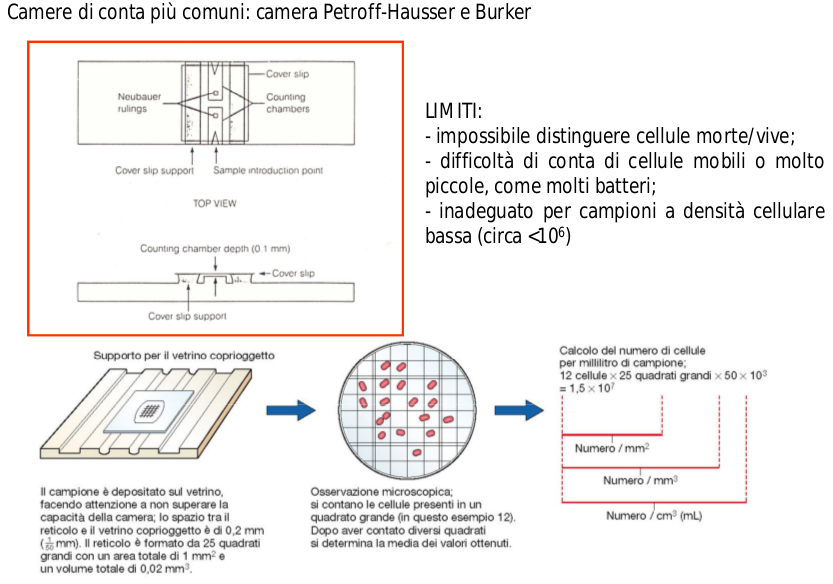
\includegraphics[scale=0.5]{img/Camere di conta.png}
\caption{Motodo di conteggio: le camere di conta}
\label{}
\end{figure}

\chapter{Controllo della crescita microbica}
\section{La crescita microbica in natura}
La sopravvivenza di una popolazione nell’ambiente naturale dipende dalla sua capacità di crescere ad una velocità sufficiente da compensare la sua scomparsa dovuta a morte per predazione, parassitismo o cause naturali.\\
La crescita è un parametro rilevante per valutare l’adattamento ad una nicchia ecologica, mentre in condizioni di laboratorio la crescita è descritta dalla curva esponenziale.

Come crescono i microrganismi in natura? Ci sono diversi parametri da considerare. Il successo nella riproduzione deve essere indipendente dalla velocità di crescita che deve essere indipendente dalla morte.

Le popolazioni batteriche in natura non possono crescere indefinitamente: l’accrescimento è limitato dalle condizioni ambientali, dalle risorse, dalla competizione, dalla predazione e da altri fattori limitanti.

\begin{figure}[htp]
\centering
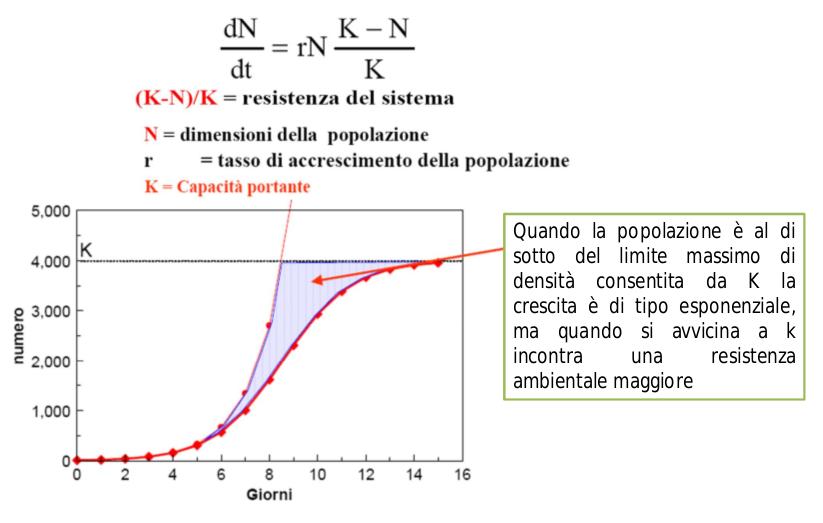
\includegraphics[scale=0.4]{img/Crescita in natura.png}
\caption{La crescita microbica in natura}
\label{}
\end{figure}

La zona in colorata nel grafico rappresenta la differenza tra la crescita esponenziale e quella logistica, rappresentando dunque la resistenza che il sistema oppone alla crescita della popolazione.

\clearpage
\section{Fattori che influenzano la crescita microbica}
\subsection{La temperatura}
La maggior parte dei batteri cresce in un intervallo termico di circa 20°C, esibendo la massima velocità di crescita ad un certo “optimum termico”.\\
In base al range di temperature di crescita i batteri possono essere divisi in gruppi:
\begin{itemize}
\item \textbf{Psicrofili}: $\sim$0–20ºC, T$\ped{opt}$ 15°C (es Polaromonas vacuolata);
\item \textbf{Mesofili}: $\sim$20–45ºC, T$\ped{opt}$ 30-37°C (es E.Coli);
\item \textbf{Termofili}: $\sim$45–80 ºC, T$\ped{opt}$ 55°C (es Bacillus Stearothermophilus);
\item \textbf{Ipertermofili}: $\sim$70–110 ºC, T$\ped{opt}$ 90-100°C (es Thermococcus Celer o Pyrolobus Fumarill).
\end{itemize}

Al di sopra della T$\ped{opt}$ si ha la denaturazione delle proteine, mentre al di sotto della T$\ped{opt}$ le membrane perdono fluidità.

\vspace{1em}
I batteri \emph{Psicrofili} e \emph{Ipertermofili} presentano adattamenti che garantiscono la loro sopravvivenza.
Ad esempio i batteri \emph{psicrofili} presentano un’elevata percentuale di acidi \emph{grassi insaturi} nella membrana plasmatica che le consentono di mantenere la fluidità, mentre i batteri \emph{ipertermofili} presentano un’elevata percentuale di acidi grassi \emph{saturi} che consentono di preservare la membrana plasmatica. Anche gli enzimi e le proteine mantengono la loro funzionalità grazie a conformazioni terziarie e quaternarie particolari.

\subsection{Il pH}
La maggior parte degli habitat naturali ha pH compreso tra 5-9. Per questo motivo i batteri che vivono a pH $\le$ 2 sono detti \textbf{acidofili}, mentre quelli che vivono a pH $\ge$ 10 sono detti \textbf{basofili}.

Ad esempio sono batteri acidofili obbligati i \emph{Solfolobus} e \emph{Thermoplasma}, i quali vivono nelle sorgenti vulcaniche con pH molto basso e T elevata, o il batterio \emph{Helicobacter pylori} che vive nel muco gastrico dello stomaco umano.

\subsection{L'attività dell’acqua}
L’attività dell’acqua (a$\ped{w}$) esprime la disponibilità di acqua e corrisponde al rapporto tra la pressione di vapore (pressione parziale a cui si verifica l’equilibrio tra fase gassosa e liquida) di una soluzione e quella dell’acqua pura. \`E un valore compreso tra 0 e 1.

A \emph{bassi valori a$\ped{w}$} ci troviamo in un ambiente \emph{ipertonico} dove i microrganismi vanno incontro a si disidratazione e morte. 
Ad \emph{alti valori di a$\ped{w}$} invece, ci troviamo in un ambiente \emph{ipotonico} dove i microrganismi crescono abbastanza agevolmente.

Tipicamente la concentrazione di soluti intracellulari è maggiore di quella presente nell’ambiente esterno (l’acqua libera va dall’esterno all’interno per osmosi). 

In condizioni di lieve ipertonicità i microrganismi reagiscono a bassi valori di a$\ped{w}$ aumentando la concentrazione intracellulare di soluti compatibili (colina, prolina, acido glutammico, betaina) che non compromettono la funzionalità cellulare ma favoriscono l’entrata di acqua.

\subsection{La concentrazione salina}
Sulla base della resistenza alle concentrazioni saline i batteri possono essere divisi in 4 gruppi:
\begin{itemize}
\item \textbf{non alofili}, richiedono un'elevata attività dell’acqua (0.9-1);
\item \textbf{alotolleranti}, possono tollerare alte concentrazioni saline (e bassa a$\ped{w}$) ma hanno un optimum di crescita a bassa concentrazione di soluti;
\item \textbf{alofili}, possono tollerare alte concentrazioni di soluti e basse a$\ped{w}$ (batteri marini 3$\%$ NaCl);
\item \textbf{alofili estremi}, crescono a concentrazioni di soluti vicino alla saturazione (15-30$\%$) (Halobacterium spp., Bacteriorodopsina).
\end{itemize}

\subsection{La disponibilità di ossigeno}
I batteri possono essere:
\begin{enumerate}
\item  \textbf{aeirobi obbligati}, necessitano di O$\ped{2}$ per il loro metabolismo aerobico;
\item \textbf{anaerobi obbligati}, l'O$\ped{2}$ risulta tossico per questi organismi. Il loro metabolismo è anaerobico (es. Clostridium Tetani);
\item \textbf{anaerobi o aerobi facoltativi}, l'O$\ped{2}$ non è tossico per questi organismi perchè sono in grado di compiere sia la respirazione anaerobica che aerobica;
\item \textbf{microaerofili}, tollerano l'O$\ped{2}$ se a basssa pressione, hanno un metabolismo anaerobico;
\item \textbf{anaerobi aerotolleranti}, l'O$\ped{2}$ non risulta tossico anche se il loro metabolismo è anaerobico.
\end{enumerate}

\begin{figure}[htp]
\centering
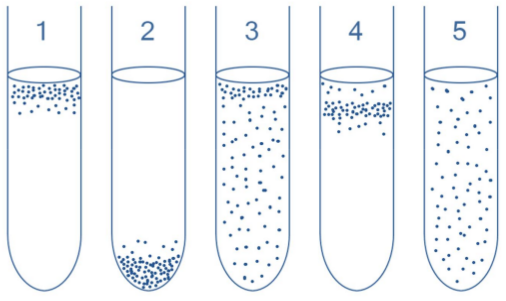
\includegraphics[scale=0.5]{img/Utilizzo ossigeno.png}
\caption{Utilizzo dell'ossigeno da parte dei batteri}
\label{}
\end{figure}

Per alcuni microrganismi l’ossigeno è fortemente tossico in quanto è un accettore di elettroni molto forte e nel processo di riduzione dell’l'O$\ped{2}$ a acqua si possono formare forme reattive dell’ossigeno \emph{(ROS, Reactive Oxygen Species)} che possono ossidare in modo incontrollato le macromolecole biologiche.

\clearpage
\begin{figure}[htp]
\centering
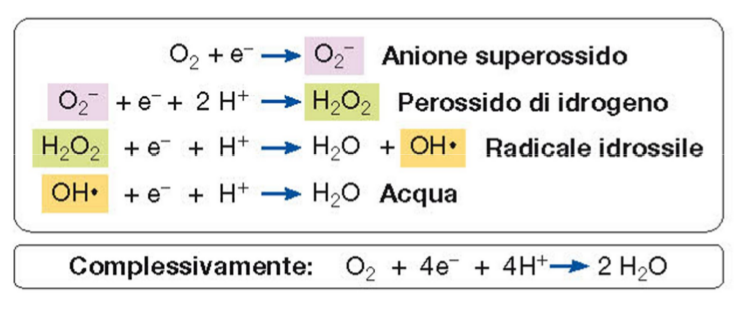
\includegraphics[scale=0.5]{img/ROS.png}
\caption{Forme reattive dell'ossigeno}
\label{}
\end{figure}
 
I batteri aerobi smaltiscono i ROS attraverso l’attività di enzimi quali:

\begin{figure}[htp]
\centering
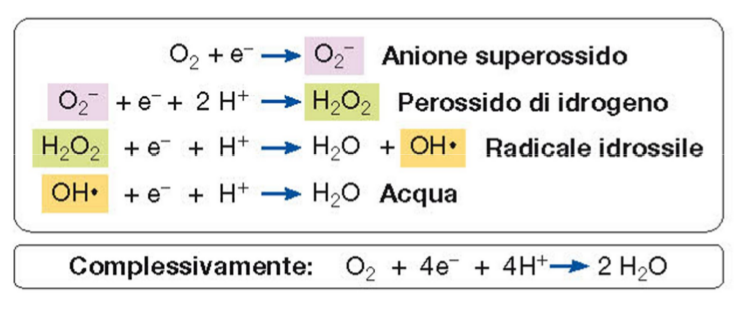
\includegraphics[scale=0.5]{img/ROS.png}
\caption{Enzimi per lo smaltimento dei ROS}
\label{}
\end{figure}

Gli enzimi utilizzati variano in base al tipo di metabolismo dell'organismo:
\begin{itemize}
\item gli \emph{aerobi obbligati} e \emph{aerobi facoltativi} contengono la \textbf{superossido dismutasi} e la \textbf{catalasi} (concentrazione O$\ped{2}$ paro al 20$\%$);
\item i \emph{microaerofili} producono solo la \textbf{superossidodismutasi} ma sono \textbf{privi di catalasi} (concentrazione O$\ped{2}$ pari al 10$\%$);
\item gli \emph{anaerobi obbligati} mancano di entrambi gli enzimi e crescono in assenza di O$\ped{2}$;
\item gli \emph{anaerobi aerotolleranti} contengono la \textbf{superossidodismutasi} e la \textbf{perossidasi}.
\end{itemize}


\section{I sistemi di coltura per i microrganismi anaerobi}
Esistono 2 sistemi di coltura dei microrganismi in anaerobiosi:
\begin{enumerate}
\item Gas-Pack per colture microbiche in anaerobiosi;
\item anaerobic glove box.
\end{enumerate}

\subsection{Controllo della crescita microbica}
La cinetica di morte dei microrganismi segue un andamento esponenziale: la popolazione microbica esposta ad un agente letale decresce ad intervalli di tempo regolari. 

Il \textbf{tempo di riduzione decimale (D)} è il tempo necessario per ridurre la carica batterica di 10 volte.

\begin{figure}[htp]
\centering
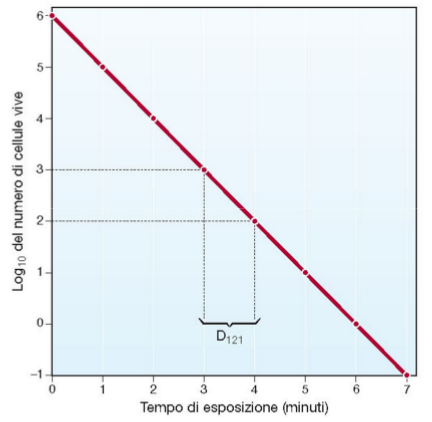
\includegraphics[scale=0.5]{img/Tempo di riduzione decimale.png}
\caption{Grafico di D}
\label{}
\end{figure}

L’efficacia di un metodo di controllo per la presenza della carica batterica e della sua morte dipende:
\begin{enumerate}
\item dalla carica microbica iniziale;
\item dalla composizione della popolazione microbica;
\item dal metodo di controllo usato;
\item dalla durata dell’esposizione.
\end{enumerate}

\`E importante disporre di metodi finalizzati all’eliminazione o alla riduzione della vita microbica presente in specifici contesti come:
\begin{itemize}
\item industria alimentare;
\item industria farmaceutica;
\item cura della salute (infezioni nosocomiali = ospedaliere);
\item sistemi di potabilizzazione e distribuzione delle acque.
\end{itemize}

Esistono diversi metodi per controllare e prevenire la carica e la crescita batterica. Tra cui:
\begin{itemize}
\item \textbf{sterilizzazione}. \`E un processo finalizzato all’eliminazione di tutti i microrganismi viventi in ambienti o su substrati (Es. sala chirurgica, farmaci, terreni di coltura);
\item \textbf{sanitizzazione}. \`E un processo finalizzato alla riduzione della carica microbica entro limiti di sicurezza;
\item \textbf{antisepsi}. \`E un processo finalizzato alla riduzione della carica microbica totale e all’eliminazione dei patogeni.
\end{itemize}


\subsubsection{La sterilizzazione}
La sterilizzazione (dal latino \emph{``sterilis''}, ovveri incapace di prole) è un processo con cui vengono distrutte o rimosse da un oggetto o da un habitat tutte le cellule viventi, le spore e i virus.

La sterilizzazione può essere ottenuta: 
\begin{itemize}
\item con \textbf{metodi fisici} come il calore (secco o umido); 
\item con \textbf{radiazioni} come raggi UV, raggi o filtrazione;
\item con \textbf{metodi chimici} come l'ossido di etilene.
\end{itemize}

La scelta del metodo di sterilizzazione dipende dal materiale da trattare. 

Il calore è da sempre uno dei mezzi più utilizzati per la sterilizzazione. La sterilizzazione al calore può essere:
\begin{enumerate} 
\item al \textbf{calore secco}. Esistono diversi mezzi per effettuarla tra cui:
\begin{itemize}
\item \textbf{stufa a circolazione d’aria}, viene utilizzata per la vetreria e strumenti in metallo, con il materiale avvolto in fogli di alluminio, carta speciale o in contenitori (180°C per 120 min);
\item \textbf{inceneritore}, usato per sterilizzare abiti, materiale usa e getta e rifiuti biologici;
\item \textbf{fiamma diretta} per sterilizzare le anse da microbiologia.
\end{itemize} 

\item al \textbf{calore umido} (per substrati, vetreria, materiali in plastica). Questa sterilizzazione viene effettuata in \textbf{autoclavi verticali o orizzontali} (121°C con 1 atm. di sovrappressione, per 15-20 min).

I tempi e le temperature di trattamento sono più ridotti nella sterilizzazione al calore umido perché:
\begin{itemize}
\item i microrganismi in forma essiccata sono più resistenti;
\item la trasmissione del calore è più efficace in vapore d’acqua.
\end{itemize}

\end{enumerate}

Durante ogni intervallo di tempo viene uccisa una uguale frazione di popolazione microbica

\clearpage
\begin{figure}[htp]
\centering
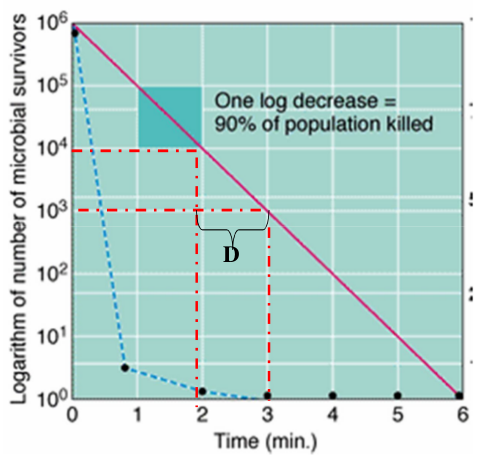
\includegraphics[scale=0.5]{img/Modello di morte microbica.png}
\caption{Modello di morte microbica}
\label{}
\end{figure}


\textbf{D} è il tempo di riduzione decimale, ovvero il tempo in minuti richiesto perché si verifichi una riduzione di 10 volte il numero di cellule viventi presenti. \`E inversamente proporzionale alla T.

\subsubsection{Fattori che influenzano l’efficacia della sterilizzazione}
\begin{itemize}
\item la dimensione della popolazione iniziale: popolazioni più ampie richiedono tempi di esposizione maggiori;
\item la composizione della popolazione: le cellule vegetative sono distrutte rapidamente mentre le endospore sono più resistenti;
\item le influenze ambientali: la presenza di materiali organici (sangue, feci, saliva) tende ad inibirene l’efficacia. Il calore è più efficace per sostanze con pH acidi (es: per succhi di frutta è sufficiente la pasteurizzazione);
\item il tempo di esposizione/concentrazione dell’agente sterilizzante: i trattamenti sono più efficaci se effettuati ad alte concentrazioni e per tempi prolungati. 
\end{itemize}

\subsubsection{La sterilizzazione al calore umido tramite l'utilizzo dell’autoclave}

All'interno dell'autoclave si trova del vapore sotto pressione che permette alla temperatura al suo interno di raggiungere i 121ºC. Questa temperatura è sufficiente a distruggere le endospore e le cellule vegetative.
Alla pressione di 1 atm il vapore raggiunge una T di 121 °C alla quale le più resistenti spore batteriche vengono distrutte in 5-10 min. 

L'autoclave presenta una resistenza che scalda l’acqua portandola a 100°. QUando l'autoclave è piena di vapore si chiude la valvola e la temperatura inizia a salire. Una volta che la temperatura è aumentata l’autoclave conta 20min in cui viene sterilizzato il suo contenuto. Finiti i minuti, annunciati dal segnale acustico, inizia ad abbassarsi la temperatura. Quando si arriva dopo i 100° si fa uscire l’ultimo vapore e si può aprire il portellone.

Nel grafico delle temperature sono presenti due curve sfalsate: una rappresenta la temperatura dell’autoclave, l’altra dell’oggetto al suo interno. All’interno dell’autoclave è presente una sonda che viene immessa in una bottiglia contenente acqua in modo da sapere che temperatura hanno raggiunto i terreni. 

\begin{figure}[htp]
\centering
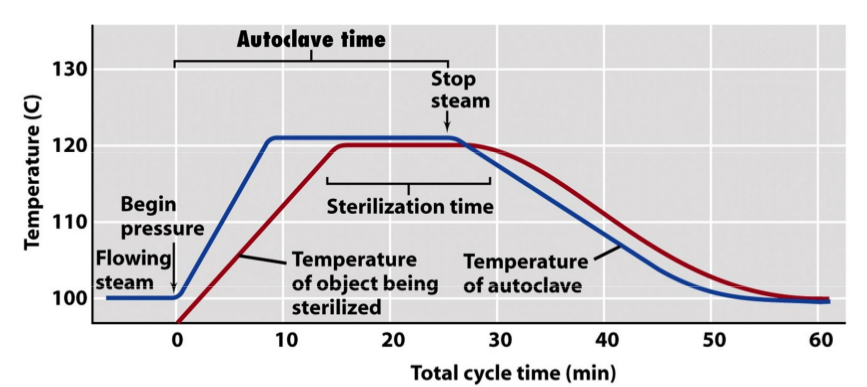
\includegraphics[scale=0.5]{img/Autoclave.png}
\caption{Sterilizzazione in autoclave}
\label{}
\end{figure}

Si può effettuare un controllo dell’efficacia dell'autoclave utilizzando un'ampolla di Bacillus stearotermophilus (ceppo PA3679): nell'autoclave si mette una provetta in cui al suo interno è presente un terreno nutrizio contenente un indicatore ed una striscetta imbevuta di spore di batteri al, il tutto dentro all'ampolla. 

Dopo la sterilizzazione nell’autoclave si rompe la provetta e se il colore dell'indicatore vira dal rosso al giallo significa che l’autoclave non ha sterilizzato bene, mentre se il colore dell'indicatore rimane rosso l’autoclave ha avuto i suoi effetti.


\subsubsection{La pasteurizzazione} 
Questo metodo di sterilizzazione su proposto da Pasteur per evitare il deterioramento dei vini dovuto a microrganismi responsabili della fermentazione lattica e acetica. 

Questo procedimento fu poi applicato al latte a fine 1800 riducendo la frequenza di TBC e brucellosi.

La pasteurizzazione, ad oggi, può essere applicata in diversi modi:
\begin{itemize}
\item quella \textbf{classica} avviene ad una temperatura di 63-66°C per 30 minuti;
\item \textbf{metodo HTST (High Temperature, Short Time)} avviene ad una temperatura di 71ºC per 15 secondi;
\item \textbf{UHT (Ultra High Temperature)} avviene ad una temperatura di 140°C per 3 secondi ed è seguita da un raffreddamento rapido.
\end{itemize}

La pasteurizzazione riduce significativamente la popolazione microbica aumentando la conservabilità dei prodotti alimentari.

\subsubsection{La sterilizzazione mediante radiazioni}
Per questo tipo di sterilizzazione possono essere usati due tipi di raggi: raggi g e i raggi ultravioletti. 

I raggi UV sono utilizzati per la sterilizzazione dell'aria (per es di una stanza), mentre i raggi g sono molto penetranti e quindi vengono utilizzati per sterilizzare il materiale in laboratorio.

\begin{figure}[htp]
\centering
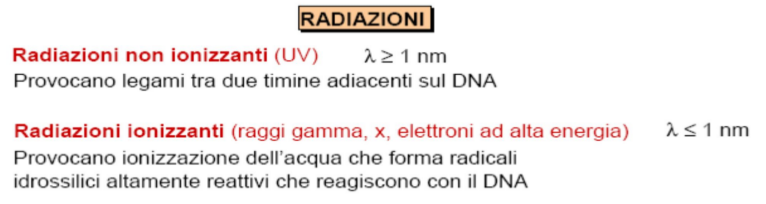
\includegraphics[scale=0.5]{img/Sterilizzazione tramite radiazioni.png}
\caption{Raggi utilizzati per la sterilizzazione}
\label{}
\end{figure}

I raggi UV hanno una scarsa capacità di penetrazione. Per questo motivo sono usati per la sterilizzare  di stanze o cappe a flusso laminare. 
Gli UV provocano danni alla cute e danneggiano gli occhi.

Le radiazioni ionizzanti invece, hanno un'alta capacità di penetrazione. Per questo motivo sono molto usate per la sterilizzazione di antibiotici, ormoni, fili da sutura, siringhe, plasticheria, ecc...


\subsubsection{La sterilizzazione mediante filtrazione}
Questo è un metodo usato per soluzioni termolabili quali vitamine, antibiotici e zuccheri. 

Le membrane filtranti possono avere differenti dimensioni dei pori. Ad esempio, membrane con pori di 0.22-0.45 $\mu$m sono usate per filtrare i batteri (ma non trattengono le spirochete, i micoplasmi e i virus), mentre membrane con pori di 0.01 $\mu$m trattengono i virus e alcune proteine.

I filtri possono essere:
\begin{itemize}
\item \textbf{a profondità}. Questi filtri sono costituiti da fibre sovrapposte di diverse sostanze (carta, vetro..). Possono essere usati come pre filtrazione per rimuovere particelle sospese, svolgono un'``azione trappola'';
\item \textbf{filtri nucleopore}. Sono sottili pellicole di policarbonato (spessore $\sim$10 mm) con pori relativamente grandi formati da trattamenti chimici “etching”. Sono utili per la microscopia poichè il materiale filtrato su trova tutto su un singolo piano.
\item \textbf{membrane filtranti convenzionali}. Sono composti polimerici come l'acetato di cellulosa o il nitrato di cellulosa. Il diametro dei pori è variabilie e svolgono un'``azione tipo setaccio''.
\end{itemize}

\clearpage
\subsubsection{Disinfezione, antisepsi}
I disinfettanti sono agenti chimici che uccidono i microrganismi. Vengono usati su oggetti inanimati.

Gli antisettico invece, sono agenti chimici usati per uccidere o inibire la crescita dei microrganismi, e sono sufficientemente non tossici per potere essere utilizzati su tessuti vivi.

\begin{figure}[htp]
\centering
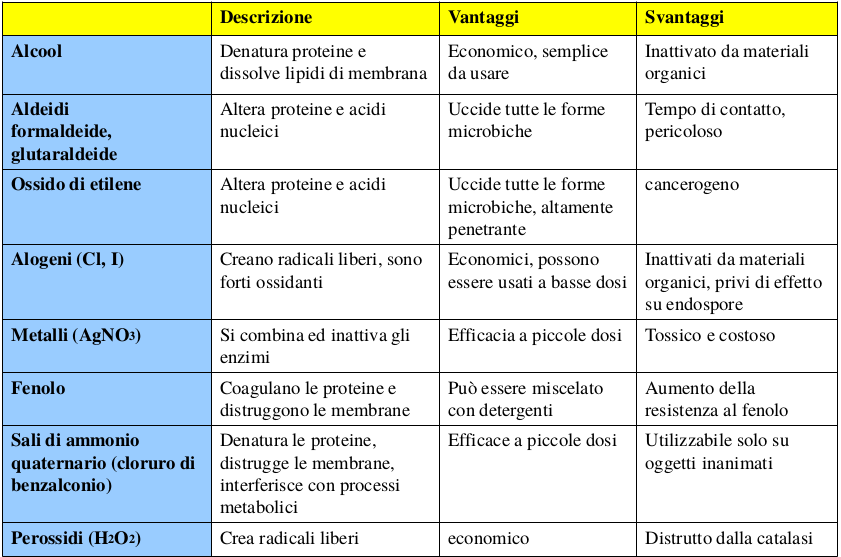
\includegraphics[scale=0.5]{img/Agenti disinfettanti.png}
\caption{Agenti disinfettanti}
\label{}
\end{figure}

\section{Agenti batteriostatici, battericidi e batteriolitici}

L'azione degli agenti antimicrobici può essere:
\begin{itemize}
\item microbicida;
\item battericida; 
\item fungicida;
\item algicida;
\item viricida;
\end{itemize}

\clearpage
Gli agenti possono variare a seconda della loro tossicità selettiva

\begin{figure}[htp]
\centering
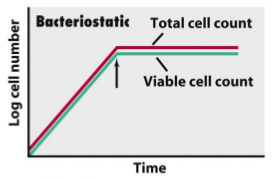
\includegraphics[scale=0.6]{img/Bacteriostatic.png}
\caption{Azione batteriostatica: inibizione della crescita cellulare microbica}
\label{}
\end{figure}

\begin{figure}[htp]
\centering
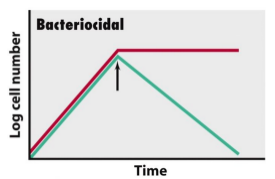
\includegraphics[scale=0.6]{img/Bacteriocidal.png}
\caption{Azione battericida: morte delle cellule vitali (es. antibiotici)}
\label{}
\end{figure}

\begin{figure}[htp]
\centering
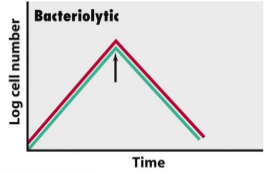
\includegraphics[scale=0.6]{img/Bacteriolytic.png}
\caption{Azione batteriolitica: causa la morte e la lisi delle cellule batteriche.}
\label{}
\end{figure}



\subsection{Gli antibiotici}
Il primo antibiotico fu scoperto grazie alle ricerche di Paul Ehlrich, finalizzate alla scoperta di un ``proiettile magico'' in grado di legarsi ai patogeni e di distruggerli. 

Lavorando sui coloranti (1904) Paul Ehlrich scoprì l’attività del Trypan Red sul\emph{ tripanosoma (protozoo)} responsabile della \emph{tripanosomiasi africana} (malattia del sonno), e osservò l’attività di composti dell’arsenico sulle spirochete della sifilide.

\vspace{1em}
Nel 1929 Alexander Fleming scoprì la penicillina. 

``Durante una ricerca con varianti di stafilococco, un certo numero di piastre erano state riposte su un angolo del bancone e venivano esaminate di tanto in tanto. Le piastre dovevano necessariamente venire aperte per poter esaminare le colture e fu così che, essendo state esposte all'aria, vennero contaminate da diversi microrganismi. Si osservò che intorno a una grossa colonia di muffa che aveva contaminato una delle piastre le colonie di stafilococco diventavano trasparenti e stavano chiaramente subendo lisi cellulare. Vennero allestite subcolture della muffa e condotti esperimenti allo scopo di accertare le eventuali proprietà della sostanza batteriolitica che si era evidentemente formata nella coltura della muffa e si era diffusa nel terreno circostante''

\vspace{1em}
Gli \textbf{antibiotici} sono prodotti naturali provenienti dal metabolismo secondario di batteri e miceti. Sono prodotti per l’80$\%$ da batteri e per il 20$\%$ da specie fungine 

I \textbf{chemioterapici} sono farmaci antibatterici ottenuti per sintesi chimica.

Gli \textbf{antibiotici semisintetici} sono molecole di origine naturale che vengono modificate chimicamente per migliorarne l’efficacia e modificarne lo spettro d’azione.

\vspace{1em}
Dal 1935 ad oggi sono stati prodotti più di 300 antibiotici, e i microrganismi hanno reagito a questo attacco evolvendo nuovi meccanismi di resistenza come:
\begin{itemize}
\item produzione di enzimi capaci di inattivare gli antibiotici;
\item alterazione della permeabilità del loro involucro;
\item alterazione del bersaglio;
\item sistemi di trasporto attivo;
\item vie metaboliche alternative (sulfamidici, antimetabolici).
\end{itemize}
                                                  


\subsubsection{I farmaci antimicrobici (ESAME!!)}
I farmaci antimicrobici si distinguono per la loro \textbf{tossicità selettiva}, ovvero per la capacità di inibire la crescita batterica senza causare danni all’organismo che lo assume. 

La tossicità selettiva può essere espressa mediante: 
\begin{itemize}
\item \textbf{dose terapeutica}. \`E la concentrazione del farmaco necessaria per il trattamento clinico di un’infezione;
\item \textbf{dose tossica}. \`E la concentrazione del farmaco oltre la quale il farmaco diventa tossico per l’ospite.
\end{itemize}

\begin{figure}[htp]
\centering

\includegraphics[scale=0.45]{img/Indice terapeutico.png}
\caption{Indice terapeutico}
\label{}
\end{figure}

Maggiore è l’indice terapeutico, migliore è l’antibiotico poichè significa che la dose tossica è alta, mentre la dose terapeutica è bassa.

I farmaci che alterano una funzione microbica assente negli eucarioti hanno indice terapeutico alto (es. penicillina).

\clearpage
\subsubsection{Lo spettro d’azione degli antibiotici}

\begin{figure}[htp]
\centering
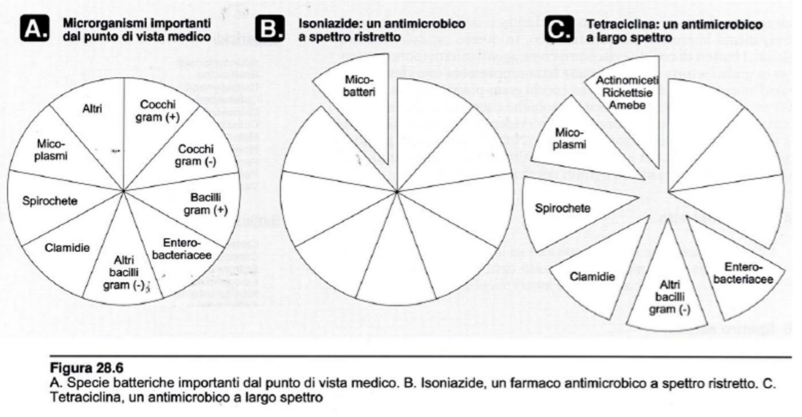
\includegraphics[scale=0.5]{img/Spettro d'azione.png}
\caption{Spettro d'azione degli antibiotici}
\label{}
\end{figure}

Lo spettro d'azione di un antibiotico, ovvero quante specie microrbiche differenti l'antibiotico è in grado di colpire, può essere:
\begin{itemize}
\item \textbf{ampio}, se la molecola è attiva verso batteri Gram+ e Gram– ;
\item \textbf{medio}, se la molecola è attiva, ad esempio, verso i batteri Gram+ e verso alcuni Gram- ;
\item \textbf{ristretto}, se la molecola è attiva, ad esempio, solamente verso batteri Gram+ o solo verso Gram–.
\end{itemize}


\subsubsection{Gli effetti degli antibiotici sui microrganismi}
Gli antibiotici interferiscono con le diverse funzioni vitali della cellula batterica.
Possono avere:
\begin{itemize}
\item un'\textbf{azione selettiva}, ovvero agire solo su alcune strutture e funzioni della cellula. Ad esemio:

\begin{itemize}
\item possono agire su strutture o vie metaboliche della cellula batterica (parete cellulare, DNA-girasi);
\item possono non essere tossici per le cellule eucariote, ed essere assunti  anche se in gravidanza.
\end{itemize}

\item un'\textbf{azione non selettiva}:
\begin{itemize}
\item se agiscono su strutture o vie metaboliche non esclusive della cellula batterica;
\item possono essere tossici per le cellule eucariote e dunque non devono essere assunti in gravidanza.
\end{itemize}

\end{itemize}

\subsubsection{Efficacia degli antibiotici}
L’efficacia di un antibiotico nei confronti di un microrganismo si valuta con un antibiogramma che può essere effettuato:
\begin{itemize}
\item su un solido (metodo di diffusione su piastra);
\item su un liquido (metodo di diluizione in brodo).
\end{itemize}

Il metodo di diffusione su piastra fornisce una stima semiquantitativa della sensibilità/resistenza di un microrganismo ad un antibiotico. Viene utilizzato il terreno di Mueller Hinton.

Tramite il metodo di incubazione del ceppo batterico in provette contenenti il substrato e dosi crescenti di antibiotico, si possono determinare:
\begin{itemize}
\item \textbf{M.I.C. o minima concentrazione inibente}. Consiste nella minima concentrazione di antibiotico capace di impedire lo sviluppo dei microrganismi ($\mu$g/ml);
\item \textbf{M.B.C. o minima concentrazione battericida}. Consiste nella minima concentrazione di antibiotico capace di indurre la morte delle cellule batteriche ($\mu$g/ml).
\end{itemize} 

Se l’antibiotico è un \emph{battericida} i valori di M.I.C. e M.B.C. coincidono, mentre se l’antibiotico è \emph{batteriostatico} i valori di MIC e MBC sono differenti (M.B.C. $\ge$ M.I.C.).

\chapter{Il metabolismo microbico}
\section{Concetti generali del metabolismo}

Il il termine \emph{``metabolismo''} (gr. $\mu$$\varepsilon$$\iota$$\alpha$$\beta$$\sigma$$\lambda$$\eta$ = trasformazione) si intende l’insieme di tutte le reazioni chimiche, organizzate in sequenze (pathways) metaboliche, che avvengono nella cellula.

Il metabolismo viene diviso in:
\begin{itemize}
\item \textbf{catabolismo}, ovvero le reazioni di \emph{demolizione delle molecole complesse} in molecole semplici con rilascio di energia;
\item \textbf{anabolismo}, ovvero la \emph{sintesi di molecole complesse} a partire da molecole più semplici con consumo di energia.
\end{itemize}

Il metabolismo si articola, generalmente, nelle seguenti fasi: 
\begin{enumerate}
\item idrolisi delle macromolecole “ambientali” mediata da esoenzimi;
\item le molecole degradate vengono trasportate all’interno della cellula;
\item i metaboliti si spostano seguendo la concentrazione intracellulare delle molecole attraverso sistemi di trasporto (attivo/passivo);
\item i metaboliti vengono trasformati, attraverso una o più vie metaboliche, in acido piruvico, metabolita intermedio universale.
\end{enumerate}

Nei sistemi biologici la produzione di energia è strettamente legata alle reazioni di ossidoriduzione (redox). Queste reazioni avvengono per via del movimento di elettroni (e$\ap{-}$) da un componente donatore a un altro componente detto accettore. 

Nella cellula il trasferimento di un e$\ap{-}$ dall’agente riducente all’agente ossidante coinvolge uno o più intermedi. Questi intermedi sono i trasportatori di e$\ap{-}$.

\vspace{1em}
I trasportatori di elettroni possono essere: 
\begin{itemize}
\item liberi, come NAD$\ap{+}$ e NADP$\ap{+}$;
\item legati a proteine della membrana plasmatica.
\end{itemize}

NAD e NADP sono i principali coenzimi redox della cellula: accettano atomi di H rilasciato dal substrato passando da forma ossidata a una forma ridotta e rilasciano protoni e elettroni nelle successive reazioni di riduzione. 
Il NAD(P) può accettare due elettroni e un protone: la forma ridotta del NAD(P)$\ap{+}$ è il NAD(P)H. 

La reazione è NAD(P) $\ap{+}$ + 2H = NAD(P)H + H$\ap{+}$.
Anche il coenzima FAD può partecipare alle reazioni biologiche di ossidoriduzione. Questo coenzima però può accettare 2 H$\ap{+}$ e 2 elettroni diventando FADH$\ped{2}$.

\vspace{1em}
I trasportatori di elettroni di mimbrana sono:
\begin{itemize}
\item NADH deidrogenasi, trasferiscono elettroni dal NADH alle flavoproteine;
\item flavoproteine, proteine contenenti flavina (coenzima derivante dalla vitamina B2);
\item proteine ferro-zolfo
\item citocromi, proteine associate a un gruppo eme contenenti Fe. Possono formare complessi con le proteine ferro-zolfo;
\item chinoni (coenzima Q), gruppo di trasportatori non proteici. 
\end{itemize}







\section{La sintesi di ATP}
Indipendentemente dalle forme di energia utilizzate (solare, chimica, ecc...) e dalla varietà dei substrati nutritivi, i meccanismi biochimici di produzione dell’ATP possono essere ricondotti a due tipologie fondamentali:
\begin{enumerate}
\item \textbf{fosforilazione a livello di substrato} (fermentazione); 
\item \textbf{fosforilazione a livello di membrana} catalizzata da ATP sintasi mediante forza proton-motrice (respirazione aerobia, anaerobia, e fotosintesi);
\end{enumerate}

\subsection{La fosforilazione a livello del substrato}
La fosforilazione a livello del substrato consiste nel trasferimento diretto di un gruppo fosfato da un substrato organico fosforilato all’ADP.

Nella fosforilazione a livello del substrato l’ATP viene sintetizzato in vari stadi durante il catabolismo di un composto organico.

Avviene frequentemente nelle fermentazioni.
La fermentazione consiste nel trasferimento diretto di un gruppo fosfato da un substrato organico fosforilato all’ADP.

\subsection{La fosforilazione a livello di membrana}
Nei vari microrganismi sono state identificate numerose catene di trasporto che condividono molti aspetti caratteristici:
\begin{itemize}
\item la presenza di una serie di trasportatori di elettroni associati alla membrana;
\item un'alternanza nella catena fra trasportatori di soli elettroni e di soli atomi di H;
\item la generazione di una forza proton-motrice come risultato della separazione di cariche attraverso la membrana (che alla fine risulta acida esternamente ed alcalina internamente).
\end{itemize}

L’idea che un gradiente protonico potesse determinare la sintesi di ATP venne proposta per la prima volta come ``teoria della chemiosmosi'' nel 1961 da Mitchell.

Nella fosforilaizone a livello di membrana invece, l'ATP può essere sintetizzato dall’ATP-sintasi di membrana che sfrutta la forza proton-motrice. La forma proton-motrice consiste in un gradiente protonico transmembrana generato da una serie di reazioni redox che coinvolgono diversi trasportatori di elettroni.

La fosforilazione a livello di membrana può essere:
\begin{enumerate}
\item \textbf{fotofosforilazione}, la forza proton-motrice è generata dalla luce;
\item \textbf{fosforilazione ossidativa}, la forza proton-motrice si genera grazie a reazioni redox tra composti chimici.
\end{enumerate}


\subsubsection{La fosforilazione ossidativa}
Nella \emph{fosforilazione ossidativa} (o trasporto di elettroni) l’ATP viene prodotto a spese della forza proton-motrice a partire da ADP e fosfato inorganico (P$\ped{i}$), durante eventi mediati dalla membrana non connessi direttamente al metabolismo di substrati specifici.

\vspace{1em}
Quando un composto organico viene mineralizzato, e$\ap{-}$ e H$\ap{+}$ sono trasferiti al NAD$\ap{-}$ che si riduce a NADH + H$\ap{-}$. Gli e$\ap{-}$ e H$\ap{+}$ sono poi trasferiti ad un accettore finale che può essere l’ossigeno o altre molecole ossidate. 

Questo trasferimento avviene in modo graduale attraverso dei trasportatori di membrana con potenziale di riduzione crescente, che nel loro insieme sono chiamati \textbf{``catena di trasporto degli elettroni''}. Tale catena di reazioni determina un movimento di H$\ap{+}$ dall’interno all’esterno della cellula (con accumulo di e$\ap{-}$ all’interno) attraverso la membrana citoplasmatica, formando un gradiente elettrochimico. 

La sintesi di ATP avviene quando gli H$\ap{+}$ accumulati all’esterno della membrana rientrano nella cellula per riequilibrare questa differenza sfruttando il complesso dell’ATP sintasi.

Questo processo avviene attraverso diverse fasi:
\begin{enumerate}
\item avviene l'ossidazione del glucosio a CO$\ped{2}$ e H$\ped{2}$O con rilascio di NADH;
\item due H$\ap{+}$ e due e$\ap{-}$ vengono trasferiti dal NADH al coenzima FMN con formazione di FMNH$\ped{2}$. I due H$\ap{+}$ vengono rilasciati all’esterno della membrana plasmatica;
\item gli e$\ap{-}$ sono usati per ridurre il gruppo Fe/S della Fe/S proteina;
\item gli e$\ap{-}$ passano dalla proteina Fe/S al chinone. Il chinone per ridursi necessita anche di 2 H$\ap{+}$ che vengono richiamati dal citoplasma;
\item si forma idrochinone che rilascia 2 H$\ap{+}$ all’esterno e cede 2 e$\ap{-}$ al citocromo b e successivamente al citocromo o.
\end{enumerate}


\clearpage
\begin{figure}[htp]
\centering
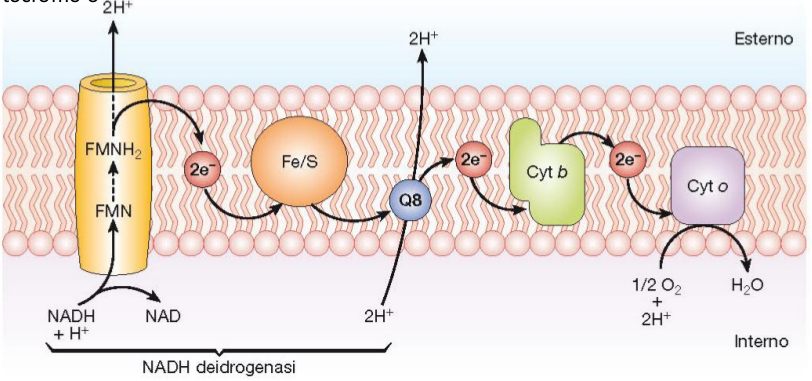
\includegraphics[scale=0.5]{img/Catena di trasporto degli elettroni.png}
\caption{La catena di trasporto degli elettroni}
\label{}
\end{figure}

\subsection{L'ATP sintasi}
Il trasporto di elettroni all’O$\ped{2}$ porta alla produzione dei componenti dell’acqua (H$\ap{+}$ ed OH$\ap{-}$), che si accumulano sulle superfici opposte della membrana.

Il risultato finale è la generazione di un gradiente di pH e di un potenziale elettrochimico attraverso la membrana, per cui l’\emph{interno} del citoplasma è \emph{elettricamente negativo} ed alcalino, mentre l’\emph{esterno} della membrana è \emph{elettricamente positivo} e acido.

Il gradiente di pH ed il potenziale elettrochimico causano l’\emph{energizzazione della membrana}. Parte di questa energia elettrica può essere conservata dalla cellula.

\vspace{1em}
Lo stato energizzato della membrana viene espresso in termini di forza proton-motrice che può essere direttamente impiegato per eseguire un lavoro utile come il trasporto di ioni, la rotazione flagellare, oppure utilizzato per la formazione di legami fosfato ad alta energia nell’ATP. 

Durante il trasporto di elettroni l’ATP viene prodotto dal processo di fosforilazione ossidativa.

L’ATP sintasi è formata da 2 componenti:
\begin{enumerate}
\item \textbf{F1}, formata da 5 subunità proteiche associata alla faccia interna della membrana. Questa subunità è immersa nel citoplasma e catalizza la reazione reversibile ADP + P = ATP;
\item \textbf{F0}, formata da 3 tipi di subunità. Questa è la componente transmembrana che forma un canale attraverso i quali passano i gli ioni H$\ap{+}$.
\end{enumerate}

Il passaggio di 3-4 H$\ap{+}$ genera ATP: gli H$\ap{+}$ entrano attraverso \emph{a} e si lega a \emph{c} protonandola e inducendo la rotazione di F1 con conseguente cambio conformazionale delle sue subunità $\alpha$ e $\beta$, le quali faranno entrare ADP e P$\ped{i}$ generando ATP che verrà rilasciato all'interno della cellula.

\clearpage
\begin{figure}[htp]
\centering
\includegraphics[scale=0.5]{img/ATP sintasi.png}
\caption{ATP sintasi}
\label{}
\end{figure}


\section{Gli organismi chemiotrofi}
Gli organismi chemiotrofi si dividono in due gruppi:
\begin{itemize}
\item i \textbf{chemiorganotrofi} o \textbf{chemioeterotrofi}, i quali ottengono energia dall’ossidazione di molecole organiche di vario tipo;
\item \textbf{chemiolitotrofi} o \textbf{chemioautotrofi}, i quali ottengono energia ossidando molecole inorganiche (es. CO$\ped{2}$).
\end{itemize}

\vspace{1em}
Alla base della diversità microbica c'è la diversità metabolica, ovvero ci sono le diverse strategie che i microrganismi hanno sviluppato per produrre ATP.

Nei \textbf{chemiotrofi}, ovvero negli organismi che nel loro metabolismo energetico utilizzano sostanze chimiche come donatori di elettroni, sono noti due meccanismi destinati alla conservazione dell'energia che hanno come risultato finale la sintesi di ATP:
\begin{enumerate}
\item la \textbf{fermentazione}. \`E un processo ossidativo in cui le reazioni redox avvengono in ambiente anaerobico e in assenza di accettori terminali di elettroni (non richiede O$\ped{2}$ o altri accettori di e$\ap{-}$). Produce energia tramite la parziale ossidazione di un substrato fermentescibile e gli elettroni sono ceduti a una molecola organica più ossidata derivante dal substrato iniziale. 
La fermentazione è una reazione di ossido-riduzione equilibrata internamente e si ha poca resa di ATP in anaerobiosi;
\item la \textbf{respirazione} (aerobia ed anaerobia). Qui è presente l’ossigeno o un’altra molecola inorganica, come accettore terminale degli elettroni. La respirazione può essere sia aerobica che anaerobica a seconda della quantità di prodotto. I substrati vengono ossidati e gli e$\ap{-}$ vengono indirizzati alla catena di trasporto degli elettroni presente sulla membrana plasmatica. Al termine della catena si trova una molecola in/organica ossidata.
\end{enumerate}


\section{Il metabolismo fermentativo dei chemioeterotrofi}
Le fermentazioni sono processi catabolici anaerobi in cui un substrato organico ridotto cede e$\ap{-}$ al NAD in una serie di reazioni redox in cui viene prodotto ATP mediante fosforilazione a livello del substrato. 
Il NADH così formato si riossiderà riducendo un intermedio della reazione che diventerà un prodotto di scarto. 

Il prodotto finale determina il nome della fermentazione:
\begin{itemize}
\item la \emph{fermentazione lattica} forma acido lattico;
\item la \emph{fermentazione alcolica} forma etanolo;
\item la \emph{fermentazione acida mista} dà etanolo, acido lattico, acido acetico...;
\item la \emph{fermentazione butandiolica} dà etanolo e butandiolo.
\item la \emph{fermentazione propionica} dà acido propionico;
\item la \emph{fermentazione butirrica} dà cido butirrico.
\end{itemize}

Molte fermentazioni hanno l’acido piruvico come intermedio di reazione.

Il piruvato si forma in seguito alla degradazione del glucosio.
La degradazione del glucosio può avvenire tramite:
\begin{itemize}
\item \textbf{glicolisi} (Embden Meyerhof Parnas, EMP);
\item \textbf{Entner Doudoroff} (via del chetogluconato);
\item \textbf{ciclo ossidativo dei pentosofosfato} (o via dell’esoso monofosfato).
\end{itemize}

\subsection{La glicolisi}
Lo \textbf{``stadio I''} consiste in una serie di riarrangiamenti preparatori, reazioni che non coinvolgono ossido-riduzioni e non rilasciano energia. 

Il glucosio viene convertito a glucosio-6P (enzima esochinasi) e questo viene convertito in fruttosio-6P (enzima glucosio-6P isomerasi), poi in fruttosio-1,6-BisP (enzima fosfofruttochinasi) che è il prodotto intermedio fondamentale della glicolisi.

Lo \textbf{``stadio II''}: il fruttosio 1,6-BisP viene scisso dall’enzima aldolasi in due molecole intermedie a tre atomi di carbonio: la gliceraldeide-3P e il suo isomero, il diidrosiacatone fosfato (anch’esso verrà convertito in gliceraldeide-3P).

La sintesi delll’ATP avviene quando ciascuna molecola di acido 1,3-difosfoglicerico viene convertita in acido 3-fosfoglicerico e successivamente, lungo la via biosintetica, quando ciascuna molecola di fosfoenolpiruvato viene convertita in piruvato. 

Nella glicolisi 2 molecole di ATP vengono consumate per due fosforilazioni del glucosio, mentre 4 molecole di ATP vengono sintetizzate (due per ciascuna molecola di ac 1,3-disfosfoglicerico trasformata in piruvato). Pertanto il risultato finale è di 2 ATP per ogni molecola di glucosio fermentata.

La glicolisi, complessivamente, porta alla sintesi di 2 molecole di ATP, 2 molecole di piruvato, 2 molecole NADH e di 6 dei 13 precursori dei costituenti cellulari.

\clearpage
\begin{figure}[htp]
\centering
\includegraphics[scale=0.6]{img/Glicolisi.png}
\caption{La glicolisi}
\label{}
\end{figure}

Il risultato della glicolisi è:
\begin{itemize}
\item il consumo di glucosio;
\item la sintesi di due molecole di ATP;
\item la sintesi di diversi prodotti di fermentazione: acidi, alcoli e sostanze gassose.
\end{itemize}

Sono note molte vie di riduzione del piruvato nei procarioti fermentanti. 

Il risultato finale però è sempre lo stesso: il NADH deve tornare nella forma ossidata, affinchè le reazioni di fermentazione che producono energia possano continuare.

Nel caso del lievito il piruvato viene ridotto ad etanolo con rilascio di CO$\ped{2}$. Nei batteri lattici, invece, esso viene ridotto in lattato con rilascio di protoni.

Durante la fermentazione viene liberata una quantità di energia relativamente piccola e vengono sintetizzate poche molecole di ATP, il quale è il prodotto fondamentale utilizzato in una larga varietà di reazioni che richiedono energia.
I prodotti di fermentazione sono invece semplici prodotti di scarto per la cellula.

\clearpage
\subsection{La via di Entner Doudoroff }
In alcuni batteri la glicolisi non è completa ed è sostituita o affiancata dalla via Entner Doudoroff.

Il batterio Zymomona mobilis usa esclusivamente questa via per il proprio catabolismo del glucosio. 

\vspace{1em}
In questa via sono presenti enzimi caratteristici come il \textbf{KDPG (2-keto-3-deossi-6-fosfogluconato aldolasi)}, e la sua resa energetica è bassa: viene prodotta 1 sola molecola di ATP per molecola di glucosio fermentata. 

I prodotti della fermentazione sono: acido piruvico, etanolo e CO$\ped{2}$.

\vspace{1em}
Questa via è effettuata da molti batteri aerobi Gram-. 

Alcuni batteri possono utilizzare questa via anche in condizioni di anaerobiosi con formazione di alcol etilico e di CO$\ped{2}$ dal piruvato, come prodotti finali. L'acido 6-fosfogluconico si trasforma in esacarbonioso, cioè in acido 2-cheto-3-deossi-6-fosfogluconico, che viene scisso in una molecola di acido piruvico e una di gliceraldeide 3-P il cui destino è la conversione ad acido piruvico lungo la via glicolitica. 

\begin{figure}[htp]
\centering
\includegraphics[scale=0.4]{img/Via di Entner Doudoroff.png}
\caption{VIa di Entner Doudoroff}
\label{}
\end{figure}.

\subsection{Il ciclo dei pentoso fosfati}
Oltre alle due vie precedentemente descritte i batteri sono dotati degli enzimi coinvolti nella via dei pentoso fosfati. Questa via porta alla sintesi di precursori metabolici essenziali quali il sedoeptulosio-7P, l'eritorosio 4P e il ribosio 5P. 

Non vengono prodotti acido piruvico e NADH ma si viene sintetizzato NADPH. Dagli intermedi (GAP) possono derivare acido piruvico e ATP se la via si accoppia alla glicolisi.


\subsection{La fermentazione}
Il processo di fermentazione può essere utilizzato per la produzione di prodotti alimentari e si suddivide in: 
\begin{itemize}
\item \textbf{alcolica}. I prodotti finali sono l'\emph{alcol etilico} e  la CO$\ped{2}$. Il piruvato viene piruvato convertito in acetaldeide con perdita di una molecola di CO$\ped{2}$, dopodichè l'acetaldeide viene convertita in etanolo) Si ha l'ossidazione del NADH e la produzione di 2 ATP;
\item \textbf{lattica} o glicolisi anaerobica. Il piruvato viene convertito direttamente in lattato con riossidazione del NADH e produzione di 2 ATP; 
\begin{itemize}
\item omolattica;
\item eterolattica;
\item fermentazione lattica dei bifidobatteri.
\end{itemize}
\end{itemize}


\subsubsection{La fermentazione omolattica}
I batteri lattici omofermentanti ossidano il glucosio tramite la glicolisi producendo 2 molecole di acido piruvico, 2 ATP e 2 NAD$\ap{+}$.

Nella fermentazione lattica il piruvato viene ridotto ad acido lattico con consumo di NADH, tramite la lattico deidrogenasi.

\subsubsection{La fermentazione eterolattica}
I batteri che eseguono questo tipo di fermentazione utilizzano una via biochimica alternativa rispetto alla glicolisi: la via del pentoso fosfato. 

Nella fermentazione eterolattica manca un enzima chiave della glicolisi, l’aldolasi. Il glucosio-6P viene ossidato a 6-fosfoglucanato che viene successivamente metabolizzato fino alla formazione di:
\begin{enumerate}
\item acido lattico;
\item etanolo;
\item CO$\ped{2}$.
\end{enumerate}

I batteri lattici eterofermentanti producono 1 molecola di ATP per ogni mole di glucosio fermentata.

\vspace{1em}
L'enzima chiave di questa via è la \textbf{fosfochetolasi} che, una volta formato il xilulosio-5P (isomero del ribulosio-5P) con la via del pentoso fosfato, permette di scinderlo in una molecola 2C (acetilfosfato) ed in una molecola 3C (gliceraldeide-3P). Queste due molecole verranno trasformate rispettivamente in etanolo e lattato.

Questa  via è caratteristica di alcuni batteri che non possiedono l'enzima fruttosio 1,6-bisfosfato aldolasi e che quindi sono incapaci di convertire il glucosio 6-P lungo la via glicolitica.  

\subsubsection{La fermentazione dei bifidobatteri}
La resa metabolica a partire da 2 molecole di glucosio è uguale a 2 molecole di acido lattico, 3 molecole di acido acetico e 5 ATP .

Da 2 molecole di glucosio si ottengono 2 molecole di Fruttosio-6P: una molecola è convertita in eritrosio-4P e acetil-P, mentre l'altra reagisce con l’eritrosio-4P a generare, dopo diverse reazioni, lo xilulosio-5P.

\subsubsection{La fermentazione alcolica}
Il lievito Saccharomyces cerevisiae, anaerobio facoltativo, è capace di ossidare il glucosio mediante glicolisi e in anaerobiosi fermentare il glucosio in etanolo e CO$\ped{2}$ .

\begin{figure}[htp]
\centering
\includegraphics[scale=0.5]{img/Fermentazione alcolica.png}
\caption{La fermentazione alcolica}
\label{}
\end{figure}

\subsubsection{La fermentazione acida mista}
La fermentazione acido mista è tipica degli enterobatteri (E. coli, Salmonella spp., Shigella spp.) e genera una \emph{miscela di acidi organici} (lattico, acetico, formico e succinico), \emph{etanolo e CO$\ped{2}$}.

\vspace{1em}
L'acido lattico si genera per riduzione diretta del piruvato.

L'acido formico si forma grazie all'enzima piruvato formiato liasi che scinde il piruvato in formiato e acetil-CoA.

La CO$\ped{2}$ deriva dalla scissione dell’acido formico.

L'etanolo si genera dalla riduzione di acetil-CoA.

L'acido acetico si forma grazie a una chinasi e a una fosfatasi a partire da Acetil-CoA.

L'acido succinico si forma per carbossilazione del piruvato.


\subsubsection{La fermentazione propionica e butirrica}
I batteri propionici (Propionibacterium shermani, P. thoeni, P. freudenreichii, P. jensenii) fermentano il lattato a:
\begin{itemize}
\item propionato;
\item acido acetico;
\item CO$\ped{2}$. 
\end{itemize}

I Clostridi fermentano il glucosio a:
\begin{itemize}
\item acido butirrico; 
\item acetone;
\item butanolo;
\item isopropanolo;
\item CO$\ped{2}$, H$\ped{2}$2;
\item acido acetico;
\item etanolo.
\end{itemize}

Aspetti applicativi fermentazione butirrica:
\begin{itemize} 
\item precursore di biocarburanti;
\item effetto anticancro (induce differenziamento cellulare e perdita della capacità neoplastica);
\item protegge le mucose dallo stress ossidativo;
\item utile per la produzione di plastiche più flessibili e resistenti di cellulosa acetato butirrato;
\item alcuni esteri dell’acido butirrico sono usati in campo alimentare come aromatizzanti;
\item sono responsabile del gonfiore tardivo nei formaggi.
\end{itemize}


\section{Il metabolismo respiratorio dei chemioeterotrofi}
La respirazione consiste nel processo metabolico in cui un donatore di elettroni (molecola organica o inorganica ridotta) è ossidato tramite una serie di reazioni al termine delle quali gli e$\ap{-}$ sono ceduti all’ossigeno o a un’altra molecola (organica o inorganica) ossidata.

L’energia che si libera è trasformata in forza proton-motrice e usata per produrre ATP. 
La respirazione si può svolgere sia in aerobiosi che in anaerobiosi, e ha un’elevata resa in ATP.

Nella respirazione anaerobica, molto diffusa nei procarioti, l’accettore terminale degli elettroni è diverso dall’ossigeno.

Nel metabolismo respiratorio il glucosio (ma anche altri mono e disaccaridi, nonché carboidrati più complessi come il glicogeno, l'amido, la cellulosa, la pectina, la cheratina, ecc) viene ossidato ad acido piruvico attraverso le tre vie prima descritte.

A questo punto l’acido piruvico formatosi viene completamente ossidato a CO$\ped{2}$ e H$\ped{2}$2O nel ciclo degli acidi tricarbossilici (TCA). Questo porta al rilascio di numerosi e$\ap{-}$ e H$\ap{+}$ che vengono trasferiti su molecole di NAD$\ap{+}$.
In questo modo si formano ATP e NADH.

Il NADH rilascia potere riducente alla catena di trasporto degli elettroni creando un gradiente protonico transmembrana. 

A seconda che l’accettore finale di e$\ap{-}$ sia l’ossigeno o un’altra molecola (es. nitrato o solfato) la respirazione viene definita aerobia o anaerobia.

\vspace{1em}
La respirazione aerobica è un processo che coinvolge sistemi di trasporto formati da trasportatori associati alla membrana che hanno due principali funzioni:
\begin{enumerate} 
\item acquistare elettroni da un donatore e trasferirli ad un accettore;
\item conservare una certa quantità di energia rilasciata durante il trasferimento degli elettroni per la sintesi di ATP.
\end{enumerate}

Nel trasporto sono coinvolti vari tipi di enzimi di ossido-riduzione disposti secondo un gradiente di potenziale redox (da negativo a positivo) a costituire la catena di trasporto degli elettroni:

\vspace{1em}
La respirazione cellulare rappresenta una via molto efficace per utilizzare al meglio l'energia accumulata dalla molecola di glucosio. Attraverso la glicolisi infatti, l'ossidazione del glucosio è parziale, e consente un guadagno netto di sole due moli di ATP. Con la respirazione cellulare invece, si ha un guadagno di altre 36 moli di ATP. 

\vspace{1em}
Le sequenze di reazione che nella respirazione seguono la glicolisi sono distinte in due stadi: il ciclo di Krebs (o ciclo dei TCA) e la catena respiratoria (o catena di trasporto degli elettroni) . 


\clearpage
\subsection{Il ciclo dei TCA}
Accoppiata all’ossidazione del glucosio c'è la produzione di 38 molecole di ATP e precursori metabolici essenziali per la biosintesi (come l'$\alpha$ -chetoglutarato, succinil CoA, ossalacetato...). 

\begin{figure}[htp]
\centering
\includegraphics[scale=0.4]{img/Ciclo dei TCA.png}
\caption{Ciclo dei TCA}
\label{}
\end{figure}


Il ciclo inizia con la decarbossilazione del piruvato, con formazione di una molecola di NADH e di un acetil-CoA (composto a due atomi di carbonio). 

L’acetil-CoA si condensa con l’ossalacetato (4 atomi di C) formando acido citrico (6 atomi di C). 

Aattarverso una serie di ossidazioni e trasformazioni, il citrato viene riconvertito in ossalacetato, che può funzionare nuovamente come accettore di acetile completando così il ciclo. 

Per ogni molecola di piruvato ossidata durante il ciclo vengono rilasciate 3 molecole di CO$\ped{2}$:
\begin{itemize}
\item una durante la formazione di acetil-CoA;
\item una dalla decarbossilazione dell’isocitrato;
\item una dalla decarbossilazione dell’alfa-chetoglutarato.
\end{itemize}
 
Gli elettroni rilasciati durante l’ossidazione degli intermedi vengono trasferiti ai coenzimi NAD$\ap{+}$ e FAD$\ap{+}$. Attraverso l’azione del sistema di trasporto degli elettroni, nella respirazione, gli elettroni vengono trasferiti all’ossigeno permettendo la completa ossidazione del glucosio a CO$\ped{2}$ con maggiore produzione di energia.

Il ciclo dell’acido citrico (così come la glicolisi) svolge dunque due importanti ruoli nella cellula: quello di produrre bioenergia tramite reazioni cataboliche, e quello di biosintesi.

Il ciclo dei TCA, infatti, porta alla sintesi di numerosi intermedi chiave che possono rispondere alle richieste biosintetiche della cellula, tra cui:
\begin{itemize}
\item l’alfa-chetoglutarato e l’ossalacetato, precursori di numerosi aminoacidi;
\item il succinil-CoA, necessario per la formazione dell’anello porfirinico dei citocromi, della clorofilla e di altri comporsti tetrapirrolici;
\item l’acetil-CoA, che costituisce il materiale di partenza per la sintesi degli acidi grassi.
\end{itemize}

Poiché il ciclo dei TCA non si limita a ossidare completamente il piruvato ma forma anche dei precursori è necessario che venga rifornito ossalacetato attraverso reazioni anaplerotiche.

Totale sono prodotte 36 molecole di ATP, per ogni molecola di glucosio consumata. Il 39$\%$ dell’energia che è presente nel glucosio viene convertita a ATP, mentre il resto è perso sotto forma di calore.

\subsection{La respirazione anaerobica}
In mancanza di O$\ped{2}$ alcuni batteri possono usare altri accettori di e$\ap{-}$ quali: nitrati, solfati, zolfo elementare, ossidi ferrici, ione manganato, fumarato... 

Esistono specifici trasportatori di e$\ap{-}$, detti ossidasi terminali. 

Il passaggio di e$\ap{-}$ dal NADH all’accettore finale attraverso i trasportatori produce forza proton motrice: la resa in ATP dipende dalla coppia ossidoriduttiva, ma è sempre inferiore alla resa dell'O$\ped{2}$.

Le respirazioni anaerobiche sono estremamente importanti dal punto di vista ecologico, perchè permettono ai microrganismi di respirare in ambienti dove l’ossigeno manca.

Esistono diversi tipi di respirazione anaerobica, e vengono divisi in base all'accettore finale degli elettroni.

\subsubsection{La denitrificazione}
La respirazione anaerobia del nitrato, ovvero la conversione del nitrato in composti gassosi dell’azoto, prende il nome di denitrificazione.

Questo è il principale processo biologico di formazione di N$\ped{2}$. 
Il nitrato (+5) viene convertito in prodotti più ridotti come: i nitriti (+3), l’ossido nitrico (+2), l'ossido nitroso (+1) e l'azoto molecolare (0) 

Gli organismi che compiono la denitrificazione vengono suddivisi in due tipi:
\begin{enumerate}
\item \textbf{anaerobi facoltativi} (Alcaligenes, Escherichia, Aeromonas Enterobacter, Bacillus, Flavobacterium, Nocardia, Spirillum, Staphylococcus e Vibrio), riducono il nitrato a \emph{nitrito} che viene poi rilasciato nel mezzo di crescita;
\item Paracoccus e Pseudomonas svolgono la seguente reazione: 

5 CH$\ped{2}$O + 4 NO$\ped{3}$$\ap{-}$ + 4 H$\ap{+}$ → 5 CO$\ped{2}$ + 2 N$\ped{2}$ + 7 H$\ped{2}$O 
\end{enumerate}

\begin{figure}[htp]
\centering
\includegraphics[scale=0.5]{img/Denitrificazione.png}
\caption{Catena di trasporto degli elettroni nella denitrificazione}
\label{}
\end{figure}

\subsubsection{La solfato riduzione dissimilativa}
Questa respirazione anaerobia è eseguita dai batteri solfato riduttori che vivono in suoli e sedimenti anossici (prevalentemente marini) e nell'intestino umano. 

Il genere più studiato è il Desulfovibrio ($\gamma$-proteobatterio): questo batterio usa alcoli, H$\ped{2}$ o acidi organici come fonte di energia ai quali sottrae e$\ap{-}$ per mezzo di idrogenasi, connesse alla catena di trasporto degli elettroni che arriva a specifiche reduttasi del solfato.

Questo procedimento avviene in 4 tappe:
\begin{enumerate}
\item avviene un'esterificazione tra un solfato e un ATP: si forma una molecola di \textbf{APS (adenosina fosfosolfato)} e una molecola PP$\ped{i}$; 
\item il PP$\ped{i}$ viene convertito a P$\ped{i}$ da un enzima fosfatasi;
\item l'APS riceve e$\ap{-}$ da H$\ped{2}$ e viene ridotto a solfito dall'enzima adenosina fosfosolfato reduttasi; 
\item il solfito, tossico per la cellula, riceve e$\ap{-}$ da H$\ped{2}$ e si riduce a solfuro grazie all'enzima solfito reduttasi.
\end{enumerate}

\subsubsection{La riduzione dissimilativa del ferro} 
Questo tipo di respirazione anaerobia è effettuata da molti batteri e Archaea. I più noti sono i \emph{Geobacter} ($\gamma$ proteobatteri) e gli \emph{Shewanella} ($\beta$ proteobatteri) che riducono il ferro (nel periplasma) per ricavare energia usando composti organici, H$\ped{2}$ e ammonio come donatori.

\subsubsection{La metanogenesi}
Gli Archaea metanogeni usano substrati per sintetizzare metano (CH$\ped{4}$). In generale l’H$\ped{2}$ è il principale donatore di elettroni.

La reazione è: 
4 H $\ped{2}$ + CO $\ped{2}$ $\longleftrightarrow$ 2 H$\ped{2}$O + CH$\ped{4}$ 


La metanogenesi è relativamente complessa e coinvolge numerosi cofattori come: il metanofurano (MF), il metanopterina (MP), il coenzima M (CoM), il Coenzima F430 (CoF430), il Coenzima F420 (CoF420) e il Coenzima B (CoB ). 

MF, MP, CoM trasportano unità C1 dalla CO$\ped{2}$ al CH$\ped{4}$.

CoF430 compie i passaggi finali della metanogenesi, mentre Co420 e CoB forniscono elettroni per ridurre CO$\ped{2}$ a CH$\ped{4}$.

La CO$\ped{2}$ è attivata dal metanofurano e ridotta a \emph{formile}.
Il formile è trasferito dal metanofurano a un enzima contenente metanopterina. Il formile viene poi ridotto a metilene e a metile in due step successivi (F420 donatore elettroni).

Il metile viene infine trasferito tramite la metil transferasi dalla metanopterina a un enzima contenente il coenzima M.

Il metil COM viene ridotto a metano dalla metil reduttasi con generazione di forza proton-motrice e ATP.


\subsubsection{Il catabolismo di lipidi, proteine e amminoacidi}
I lipidi rappresentano una fonte di C e di energia per i batteri. 

I trigliceridi vengono idrolizzati da lipasi a glicerolo e acidi grassi.

Il glicerolo viene fosforillato a fosfoglicerato, ossidato a diidrossiaceton fosfato e inviato verso la glicolisi.

Gli acidi grassi invece, vengono convertiti a esteri del CoA, subiscono $\beta$-ossidazione e vengono poi trasformati ad acetil CoA che entra nel ciclo dei TCA con produzione di NADH, FADH$\ped{2}$ ed energia.

Le proteine sono il substrato di proteasi e peptidasi che denaturano le proteine ad aminoacidi. 

Gli aminoacidi, per entrare nel metabolismo centrale, devono essere deamminati: l’ammonio viene rilasciato dalla cellula e l’acido organico risultante entra nel ciclo dei TCA.

\subsubsection{I composti organici C1 - metilotrofia}
I batteri metofili ricavano energia in aerobiosi da composti 1C quali metano, metanolo, amine metilate, dimetil etere, formaldeide e formiato. 

I metofili includono: 
\begin{itemize}
\item i \textbf{metanotrofi}, capaci di ossidare il metano;
\item i \textbf{metilotrofi}, che non possono ossidare il metano ma usano metanolo, metilamina, formiato, dimetilsolfossido e CO 
\end{itemize}

Metanotrofi sono aerobi e usano O$\ped{2}$ come accettore di elettroni.

\begin{figure}[htp]
\centering
\includegraphics[scale=0.5]{img/Passaggi metilotrofia.png}
\caption{Trasformazioni del metano duranto la respirazione}
\label{}
\end{figure}


La reazione è catalizzata dalla \emph{metano monoossigenasi (MMO)} che catalizza l’introduzione di un atomo di ossigeno nel metano mentre l’altro atomo origina acqua con gli e$\ap{-}$ derivanti da un citocromo.

\clearpage
\section{I chemiolitotrofi}
Chemiorganotrofi o chemiolitotrofi sono organismi capaci di compiere la respirazione aerobia usando come fonte di e$\ap{-}$ e di energia composti inorganici come l’H$\ped{2}$ , l’NH$\ped{3}$, il NO$\ped{2}$$\ap{-}$, S, H$\ped{}$S e Fe$\ap{+2}$. 

I chemiolitotrofi possono essere:
\begin{itemize}
\item \textbf{autotrofi} e sono indipendenti dalla sostanza organica;
\item \textbf{eterotrofi} facoltativi usano CO$\ped{2}$ e sostanza organica come fonte di C. Questi sono i batteri idrogeno ossidanti, i batteri zolfo ossidanti e i batteri che ossidano il Fe$a\ap{+2}$.
\end{itemize}

\subsection{I batteri H$\ped{2}$ ossidanti} 
L’H$\ped{2}$ si trova in ambienti ossici e anossici.

L’ossidazione aerobia dell’H$\ped{2}$ nei batteri eterotrofi è esoergonica e avviene secondo la reazione, catalizzata da una idrogenasi: 
H$\ped{2}$ + $\frac{1}{2}$ O$\ped{2}$ $\longleftrightarrow$ H$\ped{2}$O 

Mentre nei batteri autotrofi l’H$\ped{2}$ viene ossidato tramite il Ciclo di Calvin: 

6 H$\ped{2}$ + 2 O$\ped{2}$ + CO$\ped{2}$ $\longleftrightarrow$ (CH$\ped{2}$O) + 5 H$\ped{2}$O 

Un caso particolare è quello di Ralstonia eutropha che ha due idrogenasi: 
\begin{itemize}
\item catalizza la reazione sopra descritta;
\item riduce NAD$\ap{+}$ a NADH;
\end{itemize}

Ad esempio: Alcaligenes spp., Hydrogenophaga spp., Pseudomonas spp..

\subsection{I batteri zolfo e ferro ossidanti}
I solfobatteri includono specie fotosintetiche anaerobie e non fotosintetiche, alcune specie sono autotrofe obbligate, mentre altre sono eterotrofe facoltative.

L'organismo Thiobacillus thiooxidans è il tiosolfato più noto.

Alcune specie batteriche ricavano energia per la crescita dall’ossidazione del Fe$\ap{+2}$ in aerobiosi e meno frequentemente in anaerobiosi (con fotosintesi o riduzione del nitrato). 

La reazione è:
4 Fe$\ap{+2}$ + 4 H$\ap{+}$ + O$\ap{2}$ $\longleftrightarrow$ 4 Fe$\ap{+3}$ + 2 H$\ped{2}$O.


\subsection{I batteri nitrificanti} 
NH$\ped{3}$ e NO$\ped{2}$ sono composti azotati inorganici, donatori di e$\ap{-}$, che vengono ossidati da batteri nitrificanti durante la nitrificazione.

Questi batteri si dividono in due gruppi:
\begin{itemize}
\item i \textbf{batteri nitrosanti} o \textbf{ammonio ossidanti}, capaci di ossidare ossidare l’ammoniaca a nitrito (es. Nitrosomonas spp.) 

NH$\ped{4}$$\ap{+}$ + $\frac{1}{2}$ O$\ped{2}$ $\longleftrightarrow$ NO$\ped{2}$$\ap{-}$ + H$\ped{2}$O + 2 H$\ap{+}$ 

\item i \textbf{batteri nitrito ossidanti}, capaci di ossidare il nitrito a nitrato (es. Nitrobacter spp., Nitrococcus spp., Nitrospira spp.)

NO$\ped{2}$$\ap{-}$ + $\frac{1}{2}$ O$\ped{2}$ $\longleftrightarrow$ NO$\ped{3}$$\ap{-}$ 

\end{itemize}


L’azione combinata di questi due gruppi batterici comporta l’ossidazione completa dell’ammoniaca a nitrato con il trasferimento di 8 e$\ap{-}$ (il n.o. passa da -3 a +5).

L'enzima \emph{AMO (ammoniaca mono ossigenasi)} catalizza l’incorporazione di un atomo di ossigeno nell’NH$\ped{3}$ generando idrossilammina (NH$\ped{2}$OH). 

L’altro atomo di ossigeno viene ridotto a H$\ped{2}$O 

NH$\ped{3}$ + O$\ped{2}$ + 2 H$\ap{+}$ + 2e$\ap{-}$ $\longleftrightarrow$ NH$\ped{2}$OH + H$\ped{2}$O

L’NH$\ped{2}$OH viene traferita al periplasma dove viene ossidata a nitrito dalla idrossilammina ossido reduttasi (HAO) liberando 4 e$\ap{-}$, due dei quali sono usati per la generazione di potenziale mentre gli altri due tornano alla AMO per catalizzare l’ossidazione dell’ammoniaca.

I batteri nitrito ossidanti usano la NOR (nitrito ossido reduttasi) che cede e$\ap{-}$ a un citocromo con conseguente sintesi di nitrato e produzione di ATP.

\subsection{I batteri anammox}
Nell'ossidazione anaerobia dell’N (ANaerobic AMMonium Oxidation), l’NH$\ped{4}$$\ap{+}$ agisce da donatore di e$\ap{+}$ nella riduzione anerobia del nitrito (denitrificazione).

NO$\ped{2}$$\ap{-}$ + NH$\ped{4}$$\ap{+}$ $\longleftrightarrow$ N$\ped{2}$ + 2 H$\ped{2}$O 

Questo processo è stato identificato negli anni ‘90 in Brocadia anammoxidans, un planctomicete anaerobio.

Questo batterio non ha peptidoglicano ma una membrana esterna che racchiude membrane interne (con lipidi non convenzionali) incluso un organello dove avviene la reazione detto anammoxosoma:
\begin{itemize}
\item l’enzima idrazina idrolasi (HH) catalizza la combinazione tra ammonio e idrossilammina (NH$\ped{2}$OH) generando idrazina (N$\ped{2}$H$\ped{4}$); 
\item l’idrazina è ossidata dall’HZO (enzima ossidante l’idrazina) con la produzione di 4 e$\ap{-}$, 4H$\ap{+}$ e N$\ped{2}$.
\end{itemize}

\chapter{La biosintesi delle macromolecole}
\section{Il metabolismo assimilativo e biosintetico}

Esistono 4 classi di macromolece:
\begin{enumerate}
\item \textbf{acidi nucleici};
\item \textbf{proteine};
\item \textbf{polisaccaridi complessi};
\item \textbf{fosfolipidi}.
\end{enumerate}

Ognuna di queste macromolecole è formata da monomeri rispettivamente di:
\begin{enumerate}
\item \textbf{nucleotidi};
\item \textbf{amminoacidi};
\item \textbf{zuccheri};
\item acidi grassi, alcoli, zuccheri, ammine, amminoacidi...;
\end{enumerate}

Sono poi presenti 13 intermedi chiave che fanno da ponte tra degradazione e biosintesi.


\subsection{La gluconeogenesi}
La gluconeogenesi consiste nella sintesi di zuccheri a partire da molecole povere. Non presenta tutte le stesse reazioni della glicolisi condotte al contrario, poichè alcune reazioni non sono completamente reversibili:
\begin{itemize}
\item la glucosio 6 fosfatasi defosforilla il glucosio-6P a glucosio;
\item la FBP-fosfatasi defosforila il fruttosio-bisP a fruttosio-P e P$\ped{i}$; \item la PEP carbossichinasi sintetizza PEP a partire da ossalacetato e GTP.
\end{itemize}

2 acido piruvico + 4 ATP + 2 GTP + 2 NADH + 2 H$\ap{+}$ + 4 H$\ped{2}$O $\longleftrightarrow$ glucosio + 2 NAD$\ap{+}$ + 4 ADP + 2 GDP + 6 P$\ped{i}$

\subsection{Il ciclo riduttivo dei TCA} 
Desulfobacter e Chlorobium sono  batteri anaerobi fotosintetici, mentre Hydrogenobacter è un batterio aerobio. 

\vspace{1em}
Questa via porta a ossalacetato partendo da 4 CO$\ped{2}$:
\begin{itemize} 
\item PEP (C3) viene carbossilato a ossalacetato (C4) da PEP carbossilasi;
\item l'ossalacetato viene ridotto a succinato e convertito in $\alpha$-cheto glutarato;
\item l'$\alpha$-cheto glutarato è carbossilato a isocitrato e convertito a citrato;
\item il citrato (C6) viene degradato a ossalacetato (C4) e acetil CoA (C2) 
\item l'ossalacetato determina una crescita in biomassa, l'acetil CoA rigenera PEP.
\end{itemize}

Chloroflexus è un batterio fototrofo termofilo capace di fissare la CO$\ped{2}$ attraverso la via dell’idrossipropionato. 
Questa era la via arcaica dell'autotrofia. 

\subsection{L'assimilazione dell’azoto} 
L'azoto è il principale componente di proteine e acidi nucleici, e rappresenta il 14$\%$ del peso secco della cellula.

L'azoto entra nelle vie biosintetiche sotto forma di NH$\ped{3}$, che è la forma più ridotta, e permane in questa forma in tutti i costituenti cellulari. Alternativamente può essere assunto come NO$\ap{3-}$ che viene poi ridotto a NH$\ped{3}$ all’interno della cellula.

\subsubsection{L'assimilazione dell'ammoniaca} 
L’ammoniaca viene assimilata per via gassosa, e una volta all’interno della cellula viene convertita in ione ammonio e diventa substrato per tre possibili enzimi:
\begin{enumerate}
\item il \emph{carbamilfosfato sintasi}, che fa si che la CO$\ped{2}$, insieme all'NH$\ped{3}$, si converta a carbamilfosfato. Questo processo porta alla perdita di 2 molecole di ATP che vengono convertite a ADP (= perdita di P); 
\item la \emph{glutammato deidrogenasi}, presente nella reazione con l'$\alpha$- chetoglutarato + NH$\ap{4+}$ $\longleftrightarrow$ glutammato + H$\ped{2}$O con ossidazione di NADH + H$\ap{+}$ a NAD$\ap{+}$;
\item la glutamina (GS = Glutamina sintetasi ATP dipendente) e la glutamato sintasi (GOGAT = glutammato sintasi NADH dipendente).
\end{enumerate}

\subsubsection{L'assimilazione del nitrato}
Gli ioni nitrato sono trasportati attivamente nella cellula dove subiscono riduzione assimilativa ad ammonio mediante due passaggi:
\begin{enumerate}
\item HNO$\ped{3}$ + 2 e$\ap{-}$ + 2 H$\ap{+}$ $\longleftrightarrow$ HNO$\ped{2}$ + H$\ped{2}$O nitrato reduttasi assimilativa 
\item HNO$\ped{2}$ + 6 e$\ap{-}$ + 6 H$\ap{+}$ $\longleftrightarrow$ NH$\ped{3}$ + 2 H$\ped{2}$O nitrito reduttasi assimilativa
\end{enumerate}

\subsection{La fissazione dell’azoto} 
L'azoto (N$\ped{2}$) rappresenta il 78$\%$ dell'atmosfera terrestre, ed è estremamente stabile.

\vspace{1em}
La fissazione biologica dell'azoto avviene secondo questa reazione:

N$\ped{2}$ + 8 H$\ap{+}$ + 8 e$\ap{-}$ → 2 NH$\ped{3}$ + H$\ped{2}$ 

L'enzima nitrogenasi, che compie la fissazione, è composto da due proteine: 
\begin{enumerate}
\item la \emph{molibdeno-ferro proteina}, detta \textbf{nitrogenasi} (N$\ped{2}$ reduttasi, contiene 24 atomi di Fe e 2 di Mo), capace di legare l’N$\ped{2}$ e ridurlo a NH$\ped{3}$; 
\item la \emph{Fe-proteina} detta \textbf{nitrogenasi-reduttasi} che accetta il potenziale riducente e riduce la nitrogenasi.
\end{enumerate}

Questo enzima è represso dall'O$\ped{2}$ e da altre fonti di N.

La nitrogenasi-reduttasi accetta e$\ap{-}$ da un donatore a basso potenziale,la ferridossina, e lega 2 ATP, dopodichè trasferisce gli e$\ap{-}$ alla nitrogenasi.

La nitrogenasi e la nitrogenasi reduttasi formano un complesso, gli e$\ap{-}$ vengono trasferiti e l’ATP idrolizzato ad ADP + P$\ped{i}$.
 
A questo punto le due subunità si dissociano e il processo si ripete.

Quando la nitrogenasi ha ricevuto abbastanza e$\ap{-}$ (8 cicli, 16 e$\ap{-}$), lega una molecola di N$\ped{2}$ , la riduce e rilascia NH$\ped{3}$. 

La nitrogenasi accetta altri e$\ap{-}$ e il ciclo si ripete.


\subsection{L'assimilazione dello zolfo} 
Lo zolfo è presente in due amminoacidi (met e cys), in due vitamine (biotina e tiamina) e nel CoA. 

La fonte primaria di zolfo per i batteri è il solfato, piuttosto stabile, che deve essere trasformato in una forma attiva (PAPS, fosfoadenosina fosfosolfato) per  poi essere ridotto a solfito e successivamente a ione solfuro. 

Lo ione solfuro verrà incorporato nelle strutture cellulari.

\clearpage
\section{Le strategie delle vie biosintetiche}
Nella \emph{biosintesi degli amminoacidi}, lo scheletro carbonioso proviene da intermedi della glicolisi o dal ciclo dei TCA, mentre il gruppo amminico proviene dall’ammoniaca.

\begin{figure}[htp]
\centering
\includegraphics[scale=0.5]{img/Biosintesi a.a..png}
\caption{Biosintesi degli amminoacidi}
\label{}
\end{figure}

Nella \emph{biosintesi dei nucleotidi}, le purine (A, G) e le pirimidine (T, C, U) vengono sintetizzate atomo per atomo da diverse fonti di C e N a partire da ribosio 5P e ribosio 5P + ossalacetato, rispettivamente.
 
La \emph{biosintesi degli di acidi grassi (lipidi)} avviene invece nel citoplasma, grazie alla proteina per il trasporto di acile (ACP) che inserisce due atomi di C alla volta. 

L’acido grasso viene rilasciato quando ha raggiunto la sua lunghezza finale.

L'assemblaggio dei lipidi prevede la reazione tra un glicerolo e l’acido grasso.

\chapter{La genetica batterica}

L’unità funzionale dell’informazione genetica è il \textbf{gene}. 

I geni sono localizzati nei \textbf{cromosomi} o più in generale su elementi genetici.

L’informazione genetica è contenuta negli \textbf{acidi nucleici}: il \emph{DNA} (acido deossiribonucleico) e l’\emph{RNA} (acido ribonucleico).
Il DNA rappresenta la matrice genetica della cellula, mentre l’RNA permette la conversione dell’informazione contenuta nel DNA in sequenze amminoacidiche (le proteine).

DNA, RNA e proteine, sono definite \emph{macromolecole informazionali}.

\section{Il DNA e i nucleotidi} 
I monomeri degli acidi nucleici sono i nucleotidi.

Un nucleotide si compone di: 
\begin{itemize}
\item Uno \textbf{zucchero pentoso} (ribosio nell’RNA, deossiribosio nel DNA);
\item una \textbf{base azotata};
\item una \textbf{molecola di fosfato} 
\end{itemize}

Le basi azotate possono essere:
\begin{itemize}
\item \textbf{purine}, formate da due anelli eterociclici fusi; 
\item \textbf{pirimidine},formate da un anello eterociclico esatomico.
\end{itemize}

Si parla di \textbf{nucleoside}, quando si ha lo zucchero pentoso e la base azotata, mentre si parla di \textbf{nucleotide} quando si ha lo zucchero pentoso, la base azotata e il fosfato. 

\vspace{1em}
Lo zucchero pentoso e la base azotata sono legati da un legame glicosidico tra l’atomo C1 dello zucchero e l’azoto della base azotata in posizione 1 nelle pirimidine, o in posizione 9 nelle purine.
I nucleotidi sono legati tra loro dal gruppi fosfato. 
Il fosfato forma un \emph{legame fosfodiestere} con il carbonio 3’ di un nucleotide e con il carbonio 5’ di un secondo nucleotide.

\clearpage
\subsection{La struttura del DNA}
Il DNA ha una struttura a doppio filamento: i due filamenti sono tenuti insieme dai legami idrogeno che si formano tra le basi azotate (una pirimidina e una purina). 

Guanina (G) e citosina (C) presentano tre legami idrogeno, mentre adenina (A) e timina (T) presentano due legami idrogeno.

I due filamenti di DNA sono detti \emph{complementari}, poichè ogni base azotata può essere accoppiata solo ad un'altra specifica base azotata.

I filamenti di DNA complementari sono disposti in maniera \emph{antiparallela}.
Questo perchè ogni estremità 5’ termina con un gruppo fosfato e ogni estremità 3’ con un ossidrile. I due filamenti sono avvolti a formare una doppia elica in cui sono riconoscibili un solco maggiore e un solco minore. Un giro d’elica comprende 10 basi.

\section{L'informazione genetica nei procarioti}
I procarioti sono dotati di uno o più cromosomi eventualmente arricchiti da elementi genetici accessori integrati o meno nel cromosoma stesso. 

Il \textbf{nucleoide} rappresenta l'analogo strutturale del nucleo negli eucarioti.


\begin{figure}[htp]
\centering
\includegraphics[scale=0.4]{img/Il genoma procariote.png}
\caption{Organizzazione del genoma procariote}
\label{}
\end{figure}

La dimensione del DNA si esprime come numero di basi nucleotidiche o paia di basi (bp, base pairs).

Il genoma di E. coli è formato da 4640 Kbp.
 
Ogni coppia di basi ha una lunghezza di 0.34 nanometri. Questo significa che 1 Kbp è lunga 0.34 nanometri x 1000 = 340 nanometri o 0.34 $\mu$m.

Questo significa il genoma di E. coli sarebbe lungo 4640 Kbp x 0.34 $\mu$m = 1577,6 $\mu$m = 1.58 mm.

La cellula di E. coli, però, è lunga solo 2 $\mu$m e quindi il genoma deve essere superavvolto per poter stare al suo interno.

\vspace{1em}
Il \emph{superavvolgimento} e il \emph{compattamento} del DNA batterico dipendono da: 
\begin{itemize}
\item \textbf{fattori entropici}. La presenza di elevati quantitativi di RNA e proteine limitano il numero di riarrangiamenti possibili del DNA;
\item presenza di proteine di mantenimento della struttura del cromosoma (SMC) e di polipeptidi a basso PM che svolgono un ruolo simile agli istoni Eucarioti (NAP, nucleoid associated proteins);
\item topologia del DNA derivante dall’azione di due enzimi con funzione opposta: la \emph{DNA girasi} (topoisomerasi II) che introduce avvolgimenti negativi nel DNA e la \emph{DNA topoisomerasi I} che rilassa la molecola.
\end{itemize}

Le topoisomerasi di classe I interrompono il DNA su un singolo filamento, permettono la rotazione del filamento interrotto attorno all’asse del secondo filamento integro.

Le topoisomerasi di classe II determinano la rottura su entrambi i filamenti di DNA: la doppia elica integra passa attraverso la rottura che viene riparata in seguito 

\subsection{L'architettura del cromosoma batterico}
Il nucleoide è organizzato in \emph{domini} topologicamente indipendenti (la superelicità di un dominio non influenza quella degli altri). I confini di ogni dominio variano in relazione alle condizioni ambientali e alla fase di crescita. 

\vspace{1em}
La posizione delle \emph{sequenze di origine e di termine} della replicazione \emph{(ori, ter)} è precisa ma varia in base alla fase cellulare:
\begin{itemize}
\item nella cellula neoformata ori e ter sono orientate ai poli opposti della cellula;
\item nella cellula in fase intermedia ori e ter sono opposte ma in zona mediana;
\item nella cellula in fase di replicazione ori e ter sono di nuovo in zona polare opposta 
\end{itemize}

\subsection{Numero, struttura e dimensioni del cromosoma batterico} 
I procarioti sono tipicamente aploidi e il loro cromosoma può essere \emph{circolare} o \emph{lineare} (scoperto in Borrelia burgdorferi) 

La \emph{Borrelia burgdoferi} (Spirochete) agente della malattia di Lyme, trasmessa da zecche, presenta:
\begin{itemize}
\item 1 cromosoma lineare;
\item 21 plasmidi di cui 12 lineari e 9 circolari.
\end{itemize}
 
La perdita di alcuni plasmidi riduce la virulenza.

Rari sono gli esempi di batteri e Archaea poliploidi.

\vspace{1em}
Il numero di geni contenuti nel DNA genomico batterico varia da 500 a 10.000 ed è quasi tutto codificante (99.5$\%$ in E. coli). 
I ceppi di una stessa specie possono avere elevato polimorfismo (Es. E. coli EDL933 ed E. coli MG1665 non condividono il 26$\%$ delle sequenze).
 
\vspace{1em}
Genomi di grandi dimensioni garantiscono elevata versatilità metabolica (i parassiti intracellulari obbligati hanno genoma molto piccolo)

\subsection{L'organizzazione del cromosoma batterico} 
Il cromosoma di E. coli presenta un'organizzazione globale divisa in due livelli principali: macrodomini e replichores.
Nel cromosoma di E.coli, le sequenze ori e ter dividono il genoma in due metà replicative opposte chiamate \emph{replichores}.

\begin{figure}[htp]
\centering
\includegraphics[scale=0.4]{img/Replichores.png}
\caption{Replichores di E. Coli}
\label{}
\end{figure}

I cromosomi batterici differiscono per dimensione, numero e distribuzione dei geni, che nel loro insieme misurano la distanza evolutiva.

Circa il 15-17$\%$ del genoma non fa parte del genoma ancestrale della specie ma sembra sia stato acquisito a posteriori mediante trasferimento genico.

\vspace{1em}
Le \textbf{isole genomiche} sono regioni che sembrano provenire da altre specie batteriche. Le isole genomiche che hanno migliorato la performance di una specie batterica sono state selezionate positivamente e vengono definite ``fitness island''.
Queste isole genomiche sono divise in:
\begin{itemize}
\item \textbf{ecological isolands (ECI)}, codificano per enzimi degradativi e per la resistenza agli antibiotici;
\item \textbf{Saprophytic islands (SAI)}, codificano per le adesine e i  sistemi di cattura del rame;
\item \textbf{Symbiosis islands (SYI)}, codificano per gli enzimi per la fissazione dell’azoto;
\item \textbf{Pathogenicity islands (PAI)}, codificano per fattori di virulenza.
\end{itemize}

\clearpage
\subsection{Gli elementi genetici accessori}
Nelle cellule batteriche possono essere presenti anche degli elementi genetici accessori come:
\begin{itemize}
\item i plasmidi;
\item i genomi virali; 
\item le sequenze di inserzione;
\item i trasposoni; 
\item gli integroni.
\end{itemize}

Plasmidi e genomi virali possono essere integrati nel cromosoma e/o liberati nel citoplasma.
Gli elementi genetici acessori invece, sono esclusivamente integrati nel cromosoma.

Le forme citoplasmatiche replicano in modo autonomo, mentre le forme inserite sono copiate passivamente durante la replicazione del cromosoma.

\subsubsection{I plasmidi} 
I plasmidi sono molecole di DNA extracromosomali, generalmente circolari ma anche lineari, che si replicano autonomamente. 

I plasmidi conferiscono ai batteri portatori caratteristiche fenotipiche aggiuntive.

Il numero medio di plasmidi per cellula varia da poche copie (1 o 2, plasmidi a basso numero di copie) fino a numerose copie (plasmidi multicopia).

I plasmidi portano 2 informazione genetiche:
\begin{enumerate}
\item quella necessaria per la replicazione del plasmide (geni del nocciolo);
\item quelle che conferiscono al batterio particolari abilità (geni accessori). I geni accessori possono essere acquisiti o persi con notevole frequenza.
\end{enumerate}

Tutti i plasmidi hanno sequenze che segnalano l’origine di replicazione (ori), e quasi tutti hanno sequenze che regolano la frequenza di replicazione dando origine a plasmidi multicopia o meno.

Molti plasmidi possono replicarsi solo in un numero limitato di specie batteriche, altri hanno uno spettro d’ospite ampio.

\vspace{1em}
Plasmidi diversi possono coesistere nella stessa cellula, e questa viene definita \emph{compatibilità}.
 
Plasmidi identici per il nocciolo ma differenti per le caratteristiche accessorie vengono visti dall’apparato di replicazione come se fossero copie di un unico plasmide e può capitare che una delle due cellule figlie riceva il plasmide senza le caratteristiche accessorie (\emph{incompatibilità}).


\clearpage
\subsubsection{Gli elementi trasponibili: sequenze IS e trasposoni}
Gli elementi trasponibili sono entità genetiche che cambiano localizzazione nel cromosoma/plasmide in cui sono inseriti o saltano su un elemento genetico diverso mantenendo una copia nella posizione originaria.
 
Nei procarioti gli elementi trasponibili possono essere: 
\begin{itemize}
\item \textbf{sequenze di inserzione (IS)}, sono sequenze di DNA codificanti per proteine che ne promuovono la mobilità (trasposasi), fiancheggiate da brevi sequenze nucleotidiche ripetute disposte in senso opposto l’una all’altra (inverted repeat IR). All’esterno delle sequenze IS si trovano i DR (direct repeat), brevi sequenze ripetute;

\begin{figure}[htp]
\centering
\includegraphics[scale=0.4]{img/Sequenze IS.png}
\caption{Le sequenze IS}
\label{}
\end{figure}

\item \textbf{elementi criptici}, questi hanno struttura assimilabile alle IS ma sono privi della funzione di trasposizione e si muovono se riconosciuti da trasposasi batteriche

\begin{figure}[htp]
\centering
\includegraphics[scale=0.4]{img/Elementi criptici.png}
\caption{Gli elementi criptici}
\label{}
\end{figure}

\item \textbf{trasposoni semplici}, codificano sia per una caratteristica fenotipica che per proteine coinvolte nella trasposizione;

\begin{figure}[htp]
\centering
\includegraphics[scale=0.4]{img/Trasposoni semplici.png}
\caption{I trasposoni semplici}
\label{}
\end{figure}

\clearpage
\item \textbf{trasposoni complessi}, hanno il modulo centrale codificante per funzioni accessorie fiancheggiato da sequenze IS identiche codificanti per la trasposizione.

\begin{figure}[htp]
\centering
\includegraphics[scale=0.4]{img/Trasposoni complessi.png}
\caption{I trasposoni complessi}
\label{}
\end{figure}

\end{itemize}


\section{La replicazione del DNA} 
Il processo di replicazione del DNA può essere suddiviso in 3 fasi:
\begin{itemize}
\item un evento che determina l’inizio del processo;
\item una reazione iterativa che porta all’allungamento della catena;
\item una fase conclusiva che determina la terminazione della replicazione.
\end{itemize}

La sintesi del DNA parte da un'origine di replicazione identificata nel sito \emph{ori}. Con l’inizio della replicazione il DNA del sito ori viene separato localmente, portando alla formazione di una bolla costituita da due filamenti singoli definita ``\emph{forca replicativa}'', alla quale si associano proteine che formeranno il replisoma.

La replicazione dal sito ori procede in modo unidirezionale (prevalentemente) o bidirezionale.

La replicazione è \emph{semiconservativa}, questo significa che le due doppie eliche risultanti saranno costituite da un filamento parentale (stampo o guida) e da un filamento nuovo (copia).

La replicazione è \emph{discontinua}: un filamento è copiato in modo continuo per lunghi tratti, l’altro per brevi tratti discontinui adiacenti che vengono poi saldati tra loro.

L’apparato macromolecolare è costituito da un complesso multiproteico.

Il replisoma procede in modo sequenziale sintetizzando lunghe catene polinucleotidiche. Il tasso di sintesi di DNA è pressoché costante.

La replicazione bidirezionale termina in un sito del cromosoma chiamato \emph{ter} in posizione diametralmente opposta al sito ori.

La replicazione di elementi extracromosomali è spesso limitata a poche specie correlate, ma i plasmidi ad ampio spettro sono in grado di replicarsi in specie 
distanti filogeneticamente.

\clearpage
\subsection{Le proteine nella replicazione}
Esistono diverse proteine coinvolte nel processo replicativo del DNA:
\begin{itemize}
\item la \textbf{topoisomerasi} rilassa i due filamenti di DNA;
\item la \textbf{elicasi} separa i filamenti di DNA mediante la rottura dei legami idrogeno;
\item la \textbf{primasi} è una RNA polimerasi che produce i primer per l’innesco della replicazione;

\begin{figure}[htp]
\centering
\includegraphics[scale=0.6]{img/Funzione Primasi.png}
\caption{La funzione della proteina Primasi}
\label{}
\end{figure}


\item la \textbf{DNA polimerasi III (o $\alpha$} è la polimerasi replicativa;
\item la \textbf{DNA polimerasi I (o $\delta$} polimerizza in direzione 5’ $\to$ 3’ dove riempie i vuoti lasciati dai filamenti primer. Ha attività esonucleasica in direzione 3’ $\to$ 5’;
\item la \textbf{ligasi} forma un legame fosfodiestere tra l’estremità 3’ -OH di un nucleotide e la 5’ -P del nucleotide adiacente.
\end{itemize}

\clearpage
\begin{figure}[htp]
\centering
\includegraphics[scale=0.5]{img/Proteine replicazione.png}
\caption{Le proteine coinvolte nella replicazione del DNA}
\label{}
\end{figure}


\subsection{L'inizio della replicazione} 
Il sito \emph{oriC} di E. coli è  formato da 250 pb con 4 siti di legame, detti \textbf{DNA box}, per la proteina iniziatrice \textbf{DNAa} (proteina che promuove la denaturazione del DNA di \emph{ori} consumando ATP) orientate in modo inverso una verso l’altra, delle quali tre con alta affinità di legame e una con bassa affinità. 

Alla sinistra ci sono tre zone di 13 pb ricche in A e T (legame poco stabile) che favoriscono l’apertura della doppia elica.

\vspace{1em}
La \emph{DNAa} si lega alla \emph{DNAa box} formando un «complesso d’inizio» con idrolisi di ATP: l’energia che si genera è usata per srotolare l’elica a livello delle regioni ricche di AT.

L'apertura dell’elica viene mantenuta dalla \emph{DNAb (elicasi)} che rompe i legami idrogeno e permette l’avanzamento della forca replicativa.

Il \emph{complesso DNAa-DNA} continua l’avanzamento fino alle 3 zone ricche di AT generando due filamenti singoli.
Ad ognuno dei due filamenti si associa un \emph{complesso di proteine DNAb-DNAc}, dopodichè avviene il rilascio della proteina \emph{DNAc}, mentre la \emph{DNAb} continua la sua attività in direzione 5’ $\to$ 3’ con idrolisi di ATP.

La \emph{primasi DNAg} innesca la sintesi del primer RNA, e le \emph{proteine SSB} contrastano l’appaiamento tra le basi. 

\clearpage
\begin{figure}[htp]
\centering
\includegraphics[scale=0.5]{img/Inizio dell replicazione.png}
\caption{L'inizio della replicazione}
\label{}
\end{figure}


\subsection{L'innesco della sintesi e allungamento del DNA} 
La DNA primasi procede sull’\textbf{elica stampo o leading strand} in direzione 3’ $\to$ 5’ e polimerizza un primer con direzionalità 5’$\to$ 3’.

L’estremità 3’-OH del primer funziona da innesco per la DNA polimerasi che sintetizza un nuovo filamento con direzionalità 5’ $\to$ 3’; la replicazione del leading strand si blocca di tanto in tanto con sintesi di un nuovo primer.

\vspace{1em}
La replicazione del \textbf{lagging strand}, invece, avviene a tratti in modo retrogrado: la DNA primasi e la DNA polimerasi sintetizzano il nuovo filamento partendo da un sito prossimale alla forca replicativa e procedono in direzione opposta a questa.
Man mano che la forca avanza si rende disponibile un altro pezzo di stampo e la sintesi riprende più avanti.

In questo modo si generano frammenti di 1,5-2 Kb detti ``\emph{frammenti di Okazaki}''.
 
I primer a RNA vengono poi rimossi da una \emph{RNAasi H}, la polimerasi I riempie i vuoti lasciati dal primer e una ligasi unisce i frammenti.

\clearpage
La DNA polimerasi agisce in direzione 5’ $\to$ 3’ su due filamenti antiparalleli.

\begin{figure}[htp]
\centering
\includegraphics[scale=0.2]{img/Leading strand.png}
\caption{La DNA polimerasi}
\label{}
\end{figure}

Tuttavia, per permettere alla DNA polimerasi di sintetizzare due filamenti antiparalleli
usando sempre la direzionalità 5’$\to$ 3’, il filamento lagging deve formare un’ansa che
orienta il nuovo DNA in sintesi nella stessa direzione del filamento leading.

\begin{figure}[htp]
\centering
\includegraphics[scale=0.2]{img/Lagging strand.png}
\caption{La DNA polimerasi sul lagging strand}
\label{}
\end{figure}

\subsection{La terminazione della replicazione del DNA}
La replicazione è molto accurata. Si stima che gli errori di incorporazione delle basi siano prodotti con frequenze comprese tra 10$\ap{-4}$ e 10$\ap{-6}$.
 
La replicazione termina in una regione di terminazione di 350 Kb fiancheggiata da 10 siti di terminazione (ter) di 23 bp attraverso il blocco dell’attività \emph{elicasi DNAb}.

\chapter{Il tresferimento genico}
\section{Il trasferimento genico orizzontale}

I meccanismi che permettono lo scambio di materiale genetico nei batteri sono tre:
\begin{enumerate}
\item la \textbf{coniugazione}, il materiale genetico viene trasferito da una cellula all’altra attraverso la formazione di un pilo sessuale;
\item la \textbf{trasformazione}, consiste nell'acquisizione di DNA presente nell'ambiente da parte della cellula batterica;
\item \textbf{trasduzione}, un batteriofago nel corso dell’infezione di una cellula batterica trasferisce geni provenienti dalla cellula batterica in cui si è precedentemente sviluppato.
\end{enumerate}

Il trasferimento genico orizzontale conferisce alla cellula nuove proprietà fenotipiche per quanto riguarda i cosiddetti \emph{``geni non essenziali''} che consentono ai batteri di colonizzare nuovi habitat.

Il trasferimento genico coinvolge 4 fasi: 
\begin{enumerate}
\item il DNA del donatore viene preparato per il trasferimento;
\item il batterio ricevente entra in contatto con il DNA donatore;
\item il DNA donatore si stabilisce nella cellula ricevente come replicone indipendente, cioè come un plasmide che si replica autonomamente, oppure integrandosi nel DNA del ricevente;
\item i geni conferiti si esprimono e conferiscono nuove caratteristiche fenotipiche al ricevente
\end{enumerate}

\subsection{La coniugazione} 
La capacità di coniugare è conferita al batterio da elementi genetici (plasmidi o trasposoni) di tipo autotrasferibile.

La coniugazione comporta un contatto tra le cellule che nei Gram - è mediato dalla presenza di pili sessuali e nei Gram + da molecole diffusibili che promuovono l’adesione tra cellule (poco noto).
 
Per spiegare la coniugazione si fa riferimento al \emph{plasmide modello F} (fattore di fertilità di E. coli K12)

In questo caso la coniugazione avviene tra una cellula che porta il \textbf{plasmide F}, detta F$\ap{+}$ e una che ne è priva F$\ap{-}$.

\clearpage
\begin{figure}[htp]
\centering
\includegraphics[scale=0.5]{img/La coniugazione.png}
\caption{La coniugazione}
\label{}
\end{figure}

Nel processo di coniugazione si riconoscono 3 fasi: 
\begin{enumerate}
\item contatto tra la punta del pilo F del donatore e un sito recettore sulla cellula ricevente. Dopo il contatto il pilo si depolimerizza, si accorcia, e tra le due cellule si forma un poro coniugativo;
\item il trasferimento coinvolge un apparato detto rilassosoma (codificato da \emph{tra I} che occupa gran parte del plasmide) costituito da un enzima che taglia il singolo filamento a livello del \emph{sito nic} contenuto in \emph{oriT} rilassando il superavvolgimento del plasmide. L’estremità 5’ del filamento rimane legata all’enzima, mentre l’estremità 3’ resta libera;
\item il rilassosoma srotola il DNA a doppia elica muovendosi in direzione 5’$\to$ 3’, si lega al poro coniugativo e si inizia la replicazione del DNA con il modello a cerchio rotante. Il filamento intatto serve da stampo per la sintesi nella cellula donatrice del filamento complementare. Infine il filamento legato al rilassosoma è spinto nel batterio ricevente dove è convertito in DNA a doppia elica.
\end{enumerate}

\clearpage
\begin{figure}[htp]
\centering
\includegraphics[scale=0.5]{img/Passaggio plasmide nella coniugazione.png}
\caption{Il passaggio del DNA nella coniugazione}
\label{}
\end{figure}

A volte il DNA del plasmide F si integra nel cromosoma batterico per ricombinazione tra sequenze IS presenti sul plasmide e sul cromosoma.

I batteri con il plasmide F integrato sono detti \textbf{Hfr} ossia \emph{``high frequency of recombination''}.

Raramente il fattore F può excidersi con un meccanismo inverso all’integrazione.





























\end{document}